% !Mode:: "TeX:UTF-8"
%!TEX program  = xelatex

\documentclass[bwprint]{gmcmthesis}
%\documentclass{cumcmthesis}
%\documentclass[withoutpreface,bwprint]{cumcmthesis} %去掉封面与编号页,电子版提交的时候使用。

\usepackage[framemethod=TikZ]{mdframed}
\usepackage{float}
\usepackage{placeins}
\usepackage{subcaption} % 子标题
%\usepackage{hyperref}
%\usepackage{tocloft}
\title{降低汽油精制过程中的辛烷值损失模型}


%参赛信息
\baominghao{20100130029} %参赛队号
\schoolname{北京邮电大学}%学校名称
\membera{唐麒淳} %队员AB
\memberb{段祥卿} %队员B
\memberc{戴维} %队员C


% \usepackage{enumitem}
% \setlist[enumerate]{listparindent=\parindent}
\begin{document}


 %生成标题
 \maketitle


% ??????????下面的暂时不要删
% 运用科学的管理方法,大胆创新 优化操作条件 操作条件 工艺商
% 操作温度 压强 物料比 催化剂的种类及剂量 
% 操作条件温和 工艺简单容易实现 经济成本低 操作费用 投资费用 环境污染少 

 %填写摘要
\begin{abstract}
本文的建立对于优化汽油精制过程中的操作条件,从而带来巨大经济效益和环境保护效益具有重要参考意义。
本文运用机器学习与贝叶斯优化等方法对RON损失模型建模问题展开研究,首先考虑不同场景设计多种策略对数据进行处理,并用特征筛选方法找到建模的12个主要变量,然后构建机器学习管线对主要变量进行建模,训练得到具有泛化能力且高鲁棒的机器学习模型,其在5折交叉验证过程中在验证集的$r^2$评级指标为0.373。用这个机器学习模型作为评价函数,通过贝叶斯优化算法的TPE算法对325个样本的RON损失值进行优化,在产品硫含量不大于5$\mu$g/g的约束条件下使得16.92\%的变量RON损失降幅大于30\%。对133号样本优化后其RON损失降幅为32.61\% 。在问题五中,使用创新性的两步A*算法找到了逐步调整主要操作变量的调整路径。


问题一:本问题首先根据时序上是否平稳来决定313与285号样本的空值填充策略,然后通过公式定义操作变量越界程度并以此为阈值删除采样样本,用3$\sigma$准则删除异常的采样样本。最后根据不同场景制定相应的空值处理策略。通过后续建模过程较高的评价指标验证了前导数据处理流程基本正确。

问题二:本问题采用特征筛选方法来寻找建模主要变量,用嵌入式的特征打分模型梯度提升树对特征进行评价,并通过对比不同的特征筛选次数进一步限定主要变量的范围,最后筛选得到了12个主要变量。通过对所得主要变量的数据分析结果和特征重要度可视化结果可以验证主要变量筛选过程的正确性。

问题三:本问题基于分布转换与LightGBM模型在12个主要变量的基础上建立RON损失模型。首先甄别出离群的异常样本并将其删除,提升了模型的综合表现。然后建立机器学习管线并进行交叉验证,通过交叉验证的结果可以验证所得模型的鲁棒性与可泛化性。

问题四:本问题首先根据问题三的方法建立一个对硫的预测模型,并根据产品硫含量不大于5$\mu$g/g的约束条件重新设计了评价函数,通过贝叶斯优化的TPE算法对325个样本的RON损失值进行优化,并得到了RON损失降幅大于30\%样本主要变量优化后的操作条件。

问题五:本问题首先将11个主要操作变量视为高维空间中的坐标点,初始坐标即为原始操作变量值,目的坐标即为问题三所求的优化值。通过A*算法逐步调整初始坐标点在每一维上的坐标值,最终找到一条由起始点到达终点的路径。在此过程中,本队创新性地将A*算法分为两步进行,这样极大地减少了运算量。

% 同时,我们的模型可以实现在调整过程中,硫产量始终不高于5ug/g,每次调整每个变量都不会超过附件四要求的变化幅度保证系统平稳运行。同时,路径中的点也不会超过各操作变量的取值范围。最终我们得到由六十四个位点构成的路径,并将他们以及对应的硫产量和辛烷值损失制成可视化图标。


%填写关键字
\keywords{ 基于模型的特征筛选\quad 梯度提升树\quad 贝叶斯优化\quad  TPE算法\quad A*算法 }
\end{abstract}

%视情况决定是否需要建立新页面
%\newpage


%设置页码???
\pagestyle{plain}

%目录 不推荐加
%\tableofcontents

%生成目录
 \tableofcontents

\newpage


%第一章节
\FloatBarrier
\section{问题重述}
\FloatBarrier
\subsection{问题背景}

汽油是小型车辆的主要燃料,汽油燃烧产生的尾气排放对大气环境有重要影响。为此,世界各国都制定了日益严格的汽油质量标准。汽油清洁化重点是降低汽油中的硫、烯烃含量,同时尽量保持其辛烷值。

我国原油对外依存度超过70\%,且大部分是中东地区的含硫和高硫原油。原油中的重油通常占比40-60\%,这部分重油(以硫为代表的杂质含量也高)难以直接利用。为了有效利用重油资源,我国大力发展了以催化裂化为核心的重油轻质化工艺技术,将重油转化为汽油、柴油和低碳烯烃,超过70\%的汽油是由催化裂化生产得到,因此成品汽油中95\%以上的硫和烯烃来自催化裂化汽油。故必须对催化裂化汽油进行精制处理,以满足对汽油质量要求。

辛烷值(以RON表示)是反映汽油燃烧性能的最重要指标,并作为汽油的商品牌号(例如89\#、92\#、95\#)。现有技术在对催化裂化汽油进行脱硫和降烯烃过程中,普遍降低了汽油辛烷值。辛烷值每降低1个单位,相当于损失约150元/吨。以一个100万吨/年催化裂化汽油精制装置为例,若能降低RON损失0.3个单位,其经济效益将达到四千五百万元。

化工过程的建模一般是通过数据关联或机理建模的方法来实现的,取得了一定的成果。但是由于炼油工艺过程的复杂性以及设备的多样性,它们的操作变量(控制变量)之间具有高度非线性和相互强耦联的关系,而且传统的数据关联模型中变量相对较少、机理建模对原料的分析要求较高,对过程优化的响应不及时,所以效果并不理想。

某石化企业的催化裂化汽油精制脱硫装置运行4年,积累了大量历史数据,其汽油产品辛烷值损失平均为1.37个单位,而同类装置的最小损失值只有0.6个单位。故有较大的优化空间。请参赛研究生探索利用数据挖掘技术来解决化工过程建模问题。




\FloatBarrier
\subsection{问题提出}

\textbf{问题1:数据处理}

请参考近4年的工业数据的预处理结果,依“样本确定方法”对285号和313号数据样本进行预处理并将处理后的数据分别加入到附件一中相应的样本号中。


\textbf{问题2:寻找建模主要变量}

由于催化裂化汽油精制过程是连续的,虽然操作变量每3 分钟就采样一次,但辛烷值(因变量)的测量比较麻烦,一周仅2次无法对应。但根据实际情况可以认为辛烷值的测量值是测量时刻前两小时内操作变量的综合效果,因此预处理中取操作变量两小时内的平均值与辛烷值的测量值对应。这样产生了325个样本。
建立降低辛烷值损失模型涉及包括7个原料性质、2个待生吸附剂性质、2个再生吸附剂性质、2个产品性质等变量以及另外354个操作变量(共计367个变量),工程技术应用中经常使用先降维后建模的方法,这有利于忽略次要因素,发现并分析影响模型的主要变量与因素。因此,请你们根据提供的325个样本数据,通过降维的方法从367个操作变量中筛选出建模主要变量,使之尽可能具有代表性、独立性(为了工程应用方便,建议降维后的主要变量在30个以下),并请详细说明建模主要变量的筛选过程及其合理性。

\textbf{问题3:建立辛烷值(RON)损失预测模型}

采用上述样本和建模主要变量,通过数据挖掘技术建立辛烷值(RON)损失预测模型,并进行模型验证。

\textbf{问题4:主要变量操作方案的优化}

要求在保证产品硫含量不大于5μg/g的前提下,利用模型获得325个数据样本中,辛烷值(RON)损失降幅大于30\%的样本对应的主要变量优化后的操作条件。

\textbf{问题5:模型的可视化展示}

工业装置为了平稳生产,优化后的主要操作变量往往只能逐步调整到位,请你们对133号样本,以图形展示其主要操作变量优化调整过程中对应的汽油辛烷值和硫含量的变化轨迹。



%第二章节
\FloatBarrier
\section{模型假设}


%有序列表 这里写论文的模型假设
%左侧缩进可能还需要调整
\begin{enumerate}[itemindent=20pt]
	\item 题干描述的空值为0。
	\item 不考虑本题所给数据以外信息对辛烷值损失与硫含量的影响。
	\item 变量的取值范围由附件四的规定值及附件一的实际取值共同决定。
	\item 去除异常数据后,不影响数据的整体分布情况。
	\item 选择的特征参数集能够反映原数据的主要特征。
	\item 问题3训练的模型能反映操作变量与产品性质之间的关系。	
	\item 问题五假设前文搭建的硫产量及辛烷值损失预测模型可以进行准确预测。
	\item 问题五假设变量的取值范围由附件四的规定值及附件一的实际取值共同决定
\end{enumerate}


%第三章节
\FloatBarrier
\section{符号说明}


\begin{table}[hp]
    \centering
    \caption{论文中用到的符号定义}
	\begin{tabular}{cc}
	\toprule
	 \makebox[0.4\textwidth][c]{符号}	&  \makebox[0.5\textwidth][c]{意义} \\ 
	 \midrule
	 $r^2$	    & $r^2$评价指标   \\
	 H	    & 桌子高度(cm)  \\
	 \midrule
	 CV	    & 交叉验证(Cross Validation) \\
	 GBDT	& 梯度提升数(Gradient Boosting Decision tree)  \\ 
	 \bottomrule
	\end{tabular}
    \label{tab:addlabel}%
\end{table}%




%第四章节
\FloatBarrier
\section{问题分析与求解}
\FloatBarrier
\subsection{问题一:数据处理}\label{sec:data-process}

%\FloatBarrier
%\subsubsection{问题分析}

%
%由于每套装置的数据均有部分位点存在问题:部分变量只含有部分时间段的数据,部分变量的数据全部为空值或部分数据为空值。因此对原始数据进行处理后才可以使用。
%
%问题一的目标是参考近4年的工业数据的预处理结果,根据附件的样本确定方法对285号样本与313号样本的数据进行处理,并将处理后的285号样本与313号样本加入到原工业数据中。对于原工业数据的空值,我们设计了数据处理方法进行处理。


\FloatBarrier
\subsubsection{对含空值变量的分析}\label{sec:empty-analyze}

考虑到工业设备传感器失效或异常时记录值为0,在此认为0代表了工业数据中的空值。

经过分析可以发现285号样本的“新氢进装置流量”、“1\#催化汽油进装置流量”等操作变量全部为空值0,但其余操作变量不含空值。考虑到最后需要取其前2个小时的操作变量数据的平均值作为对应辛烷值的操作变量数据,所以最后汇总得到的相应的操作变量值仍是0,故暂时不对这类变量做处理,留到\ref{sec:process-all-nan}中处理。

经过分析,容易发现313号样本除了“新氢进装置流量”等操作变量与上文描述的一样也全部为空值0以外,还有部分操作变量只含有部分空值。对于这类操作变量,制定了2种处理策略:

\textbf{处理1}:对时序上基本平稳的含空值变量做均值填充

在313号样本的数据中,容易发现2个时序上基本平稳但含有空值的变量。考虑到本题确定某个样本的方法为:以辛烷值数据测定的时间点为基准时间,取其前2个小时的操作变量数据的平均值作为对应辛烷值的操作变量数据。故对于这两个变量的空值用313号样本数据的其余采样相应变量的均值来填充。


\begin{figure}[htb]
    \centering
    \begin{minipage}[c]{0.35\textwidth}
        \centering
        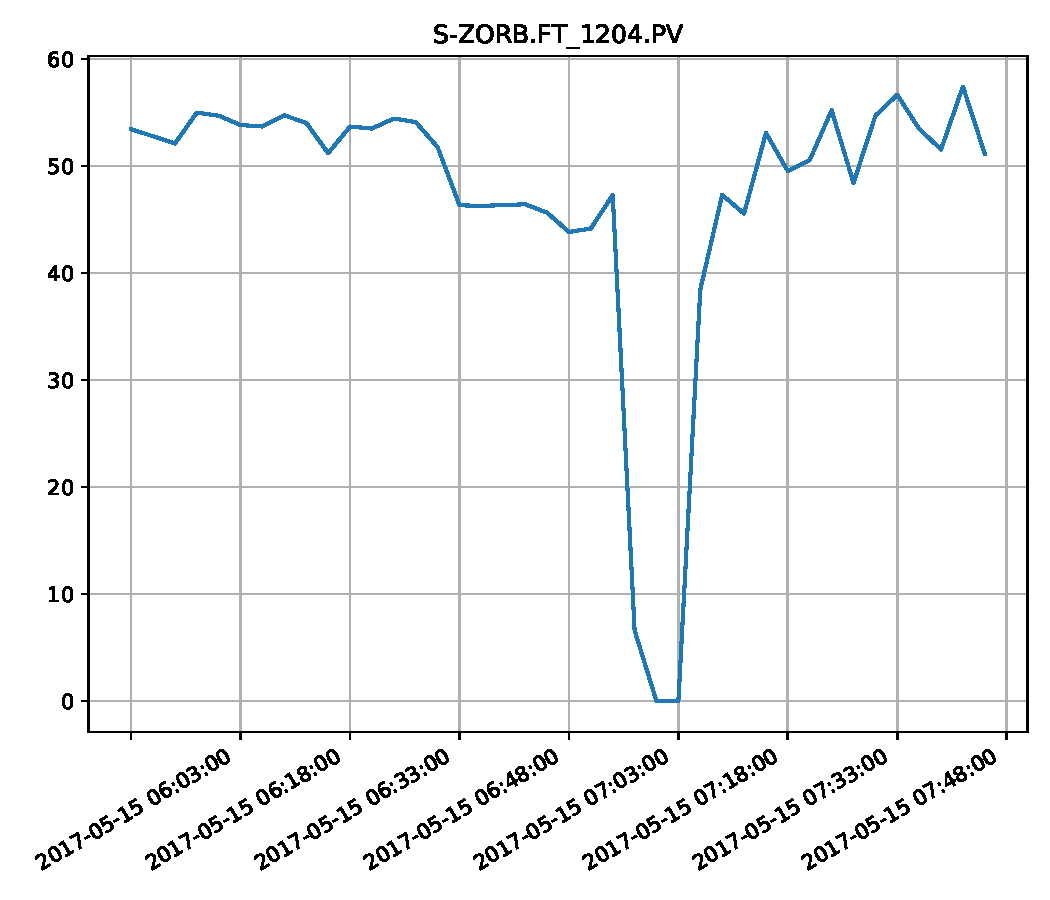
\includegraphics[height=0.2\textheight]{313-fill-1}
        \subcaption{S-ZORB.FT\_1204.PV}
    \end{minipage}
    \begin{minipage}[c]{0.35\textwidth}
        \centering
        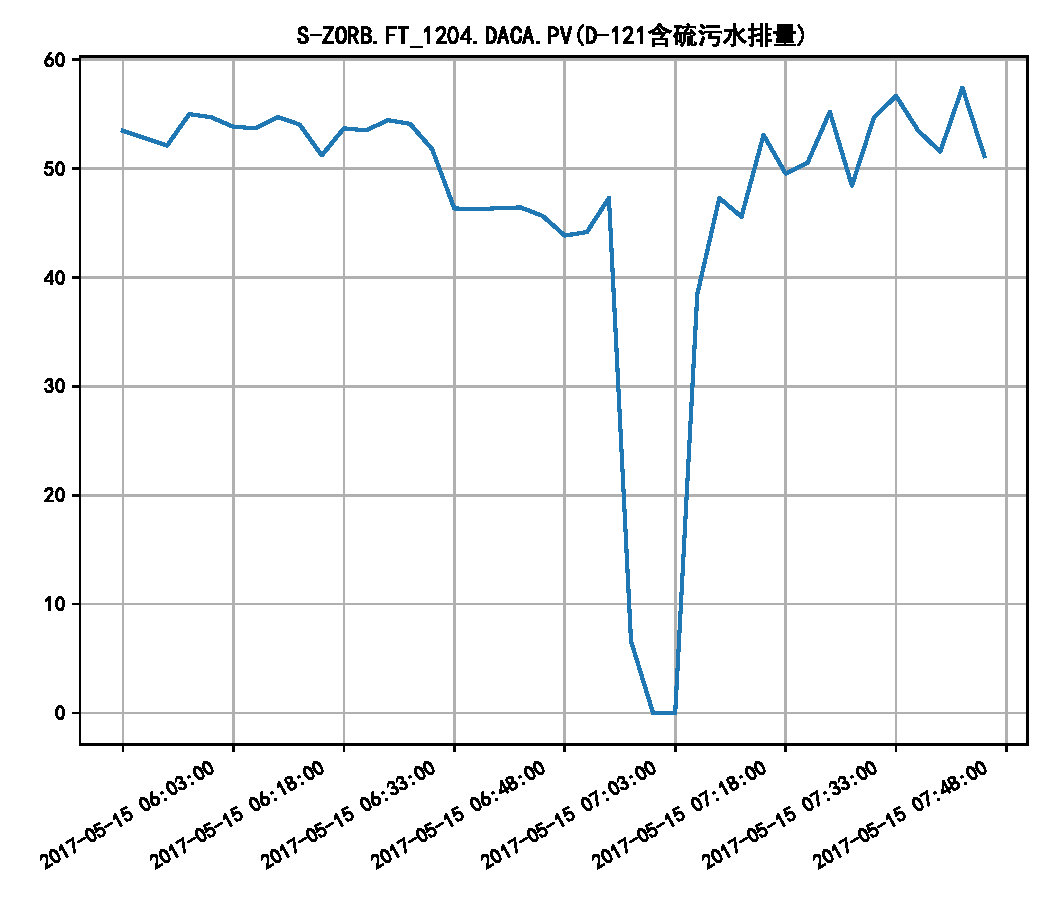
\includegraphics[height=0.2\textheight]{313-fill-2}
        \subcaption{D-121含硫污水排量}
    \end{minipage}
    \caption{313号样本处理1中的2个变量}
\end{figure}


\textbf{处理2}:对时序上杂乱或呈周期趋势的含空值变量做删除操作

在313号样本的数据中,容易发现3个时序上杂乱或呈周期趋势的含空值变量但含有空值的变量 。考虑到本题对于只含有部分时间点的位点,如果其残缺数据较多,无法补充,应将此类位点删除,所以将313号样本的这3个变量设为$NaN$,留到\ref{sec:process-all-nan}中处理。



\begin{figure}[htb]
    \centering
    \begin{minipage}[c]{0.35\textwidth}
        \centering
        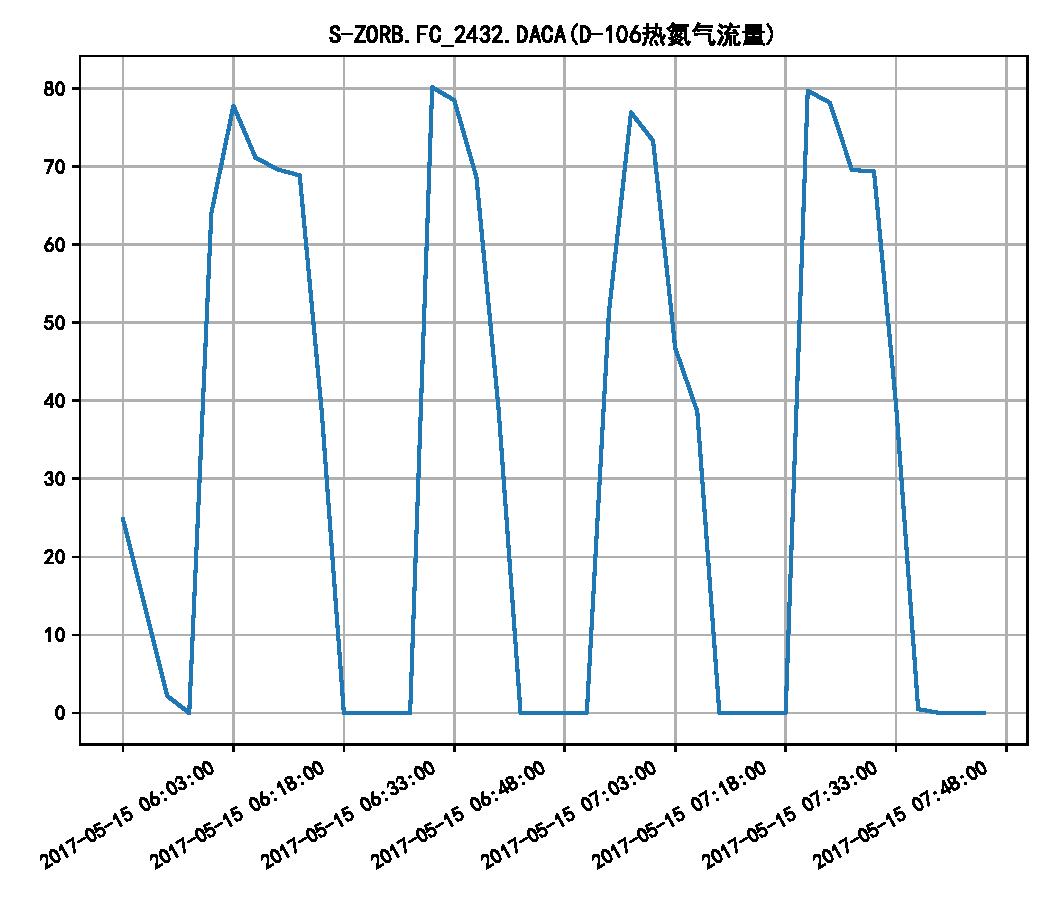
\includegraphics[height=0.2\textheight]{313-del-1}
        \subcaption{D-106热氮气流量}
    \end{minipage}
    \begin{minipage}[c]{0.35\textwidth}
        \centering
        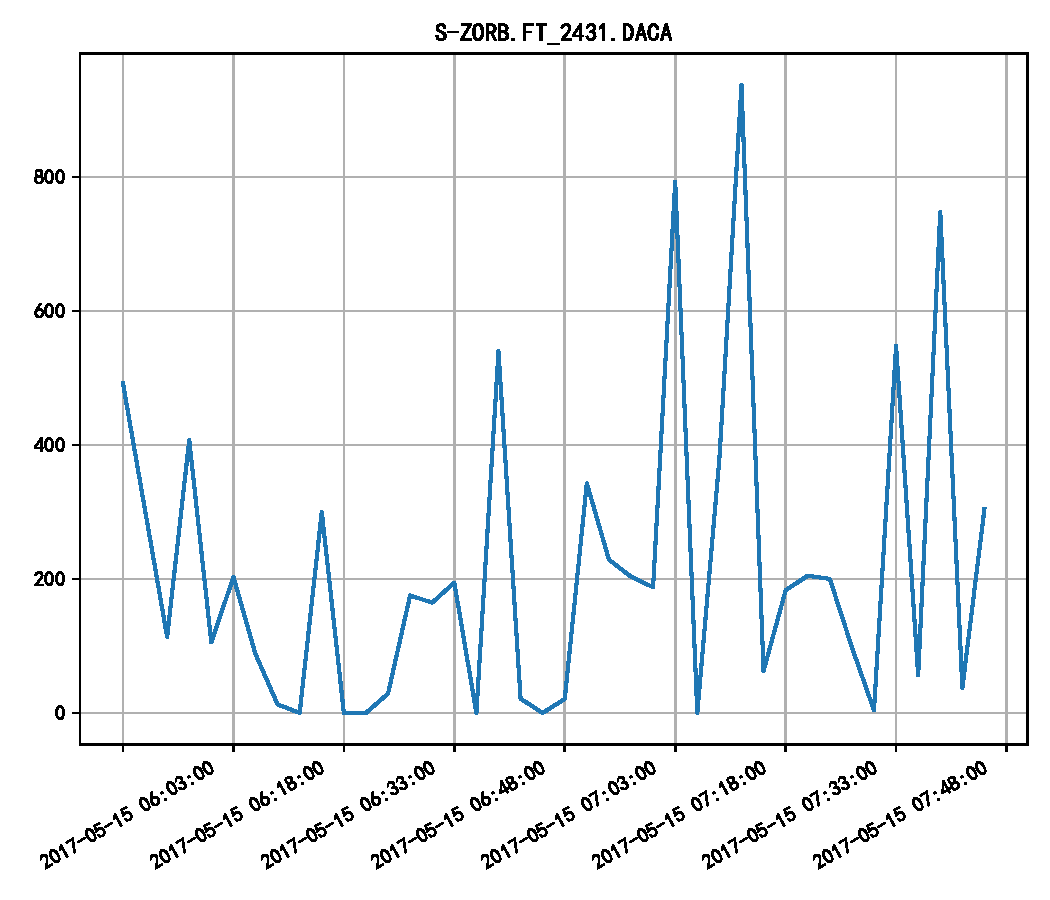
\includegraphics[height=0.2\textheight]{313-del-2}
        \subcaption{S-ZORB.FT\_2431.DACA}
    \end{minipage}
     \begin{minipage}[c]{0.35\textwidth}
        \centering
        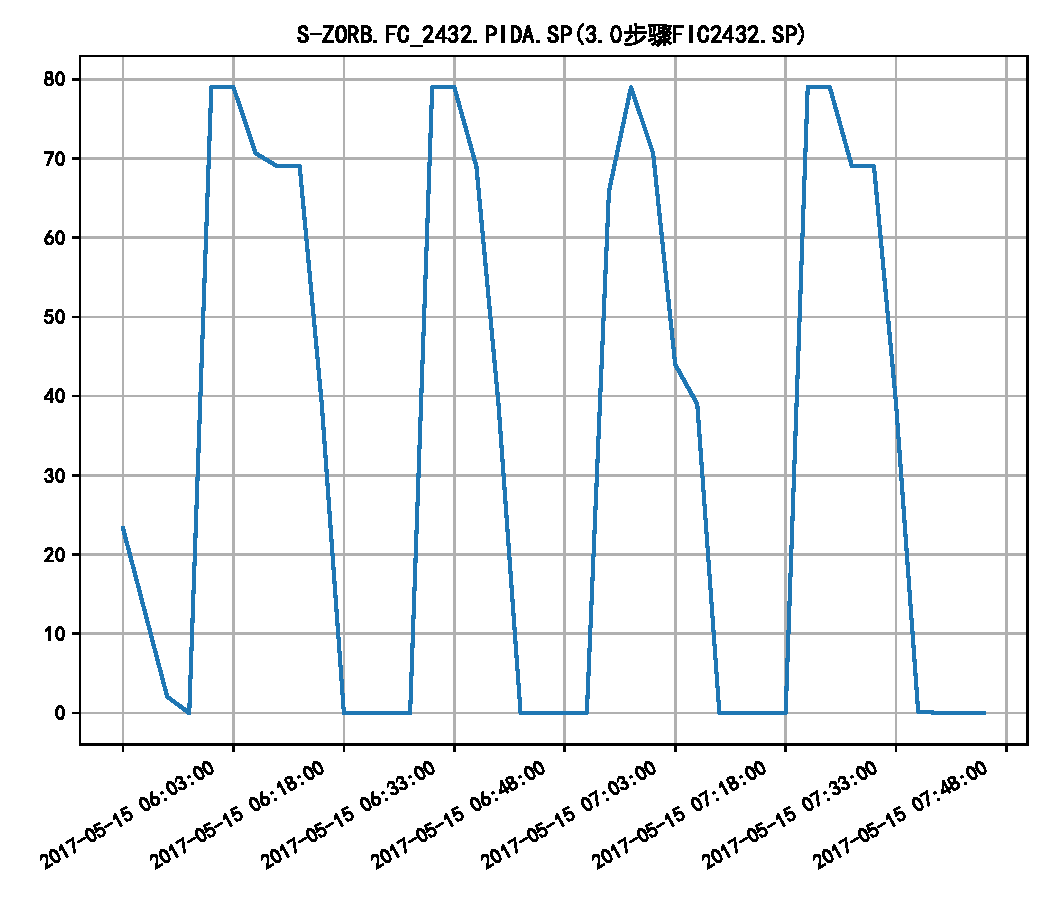
\includegraphics[height=0.2\textheight]{313-del-3}
        \subcaption{3.0步骤FIC2432.SP}
    \end{minipage}
    \caption{313号样本处理2中的3个变量}
\end{figure}




\FloatBarrier
\subsubsection{剔除不在操作范围内的样本}

考虑到“325个样本数据”中的很多样本已经超出了“354个操作变量信息”所规定的范围,于是应该进行简单的处理,用“325个样本数据”中每个操作变量的最大与最小值来扩充“354个操作变量信息”中操作变量的范围,并用扩充后的操作变量范围代替原操作变量范围。

经过计算,285样本数据中所有的采样数据都在操作变量范围内,而313样本数据仅有1个采样数据的所有变量在操作变量范围内。经过综合考虑,决定用以下公式来计算一个采样样本操出操作变量范围的程度:

\begin{equation}
	InvalidDegree=\sum^M_j{\frac{Exceed_j}{Upper_j - Lower_j}}
	\label{eq:range-invalid-degree}
\end{equation}

其中,$j$表示某采样样本的第$j$个操作变量,$M$表示共有$M$个操作变量, $Upper_j$表示操作变量$j$的上界,$Lower_j$表示操作变量$j$的下界,$Exceed_j$表示操作变量$j$超出范围的大小。

使用上述公式,对313样本的采样数据进行计算,结果如下:

\begin{table}[htb]
	\caption{313样本超出范围程度}\label{tab:001} \centering
	\begin{tabular}{ccc}
	\toprule[1.5pt]
	time &  invalid-degree &  rank \\
	\midrule[1pt]
	2017-05-15 06:57:00 &        1.986283 &     0 \\
	2017-05-15 07:24:00 &        1.868216 &     1 \\
	2017-05-15 07:18:00 &        1.533825 &     2 \\
	2017-05-15 06:33:00 &        1.514671 &     3 \\
	2017-05-15 06:54:00 &        1.298304 &     4 \\
	2017-05-15 06:51:00 &        1.057390 &     5 \\
	2017-05-15 07:21:00 &        0.876193 &     6 \\
	2017-05-15 07:51:00 &        0.866200 &     7 \\
	2017-05-15 07:48:00 &        0.770276 &     8 \\
	2017-05-15 07:54:00 &        0.658065 &     9 \\
	\bottomrule[1.5pt]
\end{tabular}
\end{table}


经过综查阅相关文献和讨论,在此决定以$InvalidDegree >= 1$为阈值,删除满足其条件的所有采样样本。



\FloatBarrier
\subsubsection{用3$\sigma$准则删除异常样本}

3$\sigma$准则:设对被测量变量进行等精度测量,得到$x_1, x_2, \ldots, x_n$,算出其算术平均值$x$及剩余误差$v_i=x_i-x (i=1, 2, \ldots , n)$,并按贝塞尔公式算出标准误差$\sigma$,若某个测量值$x_b$的剩余误差$v_b ( 1 <= b <= n )$,满足 $|v_b| = | x_b - x | > 3\sigma$,则认为$x_b$是含有粗大误差值的坏值,应予剔除。贝塞尔公式如下:

\begin{equation}\label{eq:3sigma}
	\sigma = [\frac{1}{n-1}\sum_{i=1}^{n}v_i^2]^{\frac{1}{2}} = \{\frac{[\sum^n_{i=1}x_i^2 - (\sum^n_{i=1}x_i)^2/n]}{n-1}\}^{\frac{1}{2}}
\end{equation}

根据上述公式,285样本的所有采样都满足3$\sigma$准则,而313样本有27个采样不满足其条件,故删除这些不满足条件的变量。


\FloatBarrier
\subsubsection{对工业数据中的空值变量进行处理}\label{sec:process-all-nan}

通过前述操作,将313样本和285样本经过处理后加入到325个样本的工业数据中,并将\ref{sec:empty-analyze}处理2中删除的变量设置为 $NaN$ ,待进一步的处理。

对于不同类型的情况,制定3种处理空值的策略:

\begin{equation}\label{eq:empty-strategies}
\left\{
\begin{aligned}
delete \ column, \ & if \ len(EmptyElements)>50 \ and \ mean(vector)>5 \\  
delete \ element, \ & if \ len(EmptyElements)<50 \ and \ mean(vector)>5\\  
do \ not \ process, \ & if \ mean(vector)<=5
\end{aligned}
\right.
\end{equation}

根据公式\eqref{eq:empty-strategies},对于工业数据中的空值有3种处理策略:

\newcounter{mylist}
\begin{list}{策略\themylist}{\usecounter{mylist}}
	\item 如果某列空值元素的长度 $len(EmptyElements)$ 大于50,并且这列元素的均值 $ mean(vector)$ 大于5,说明空值较多,做空值填充的意义不大,应该将此列删除。
	\item 如果某列空值元素的长度小于50,并且这列元素的均值大于5,说明空值相对较少,可以通过做空值填充保留下来。
	\item 如果这列元素的均值小于等于5,说明这列元素基本为0,0可能不是这列元素的空值,所以不做处理。
\end{list}


三种策略的处理结果数据如下:






\begin{figure}[htb]
	\centering
	\begin{minipage}[c]{0.4\textwidth}
		\centering
		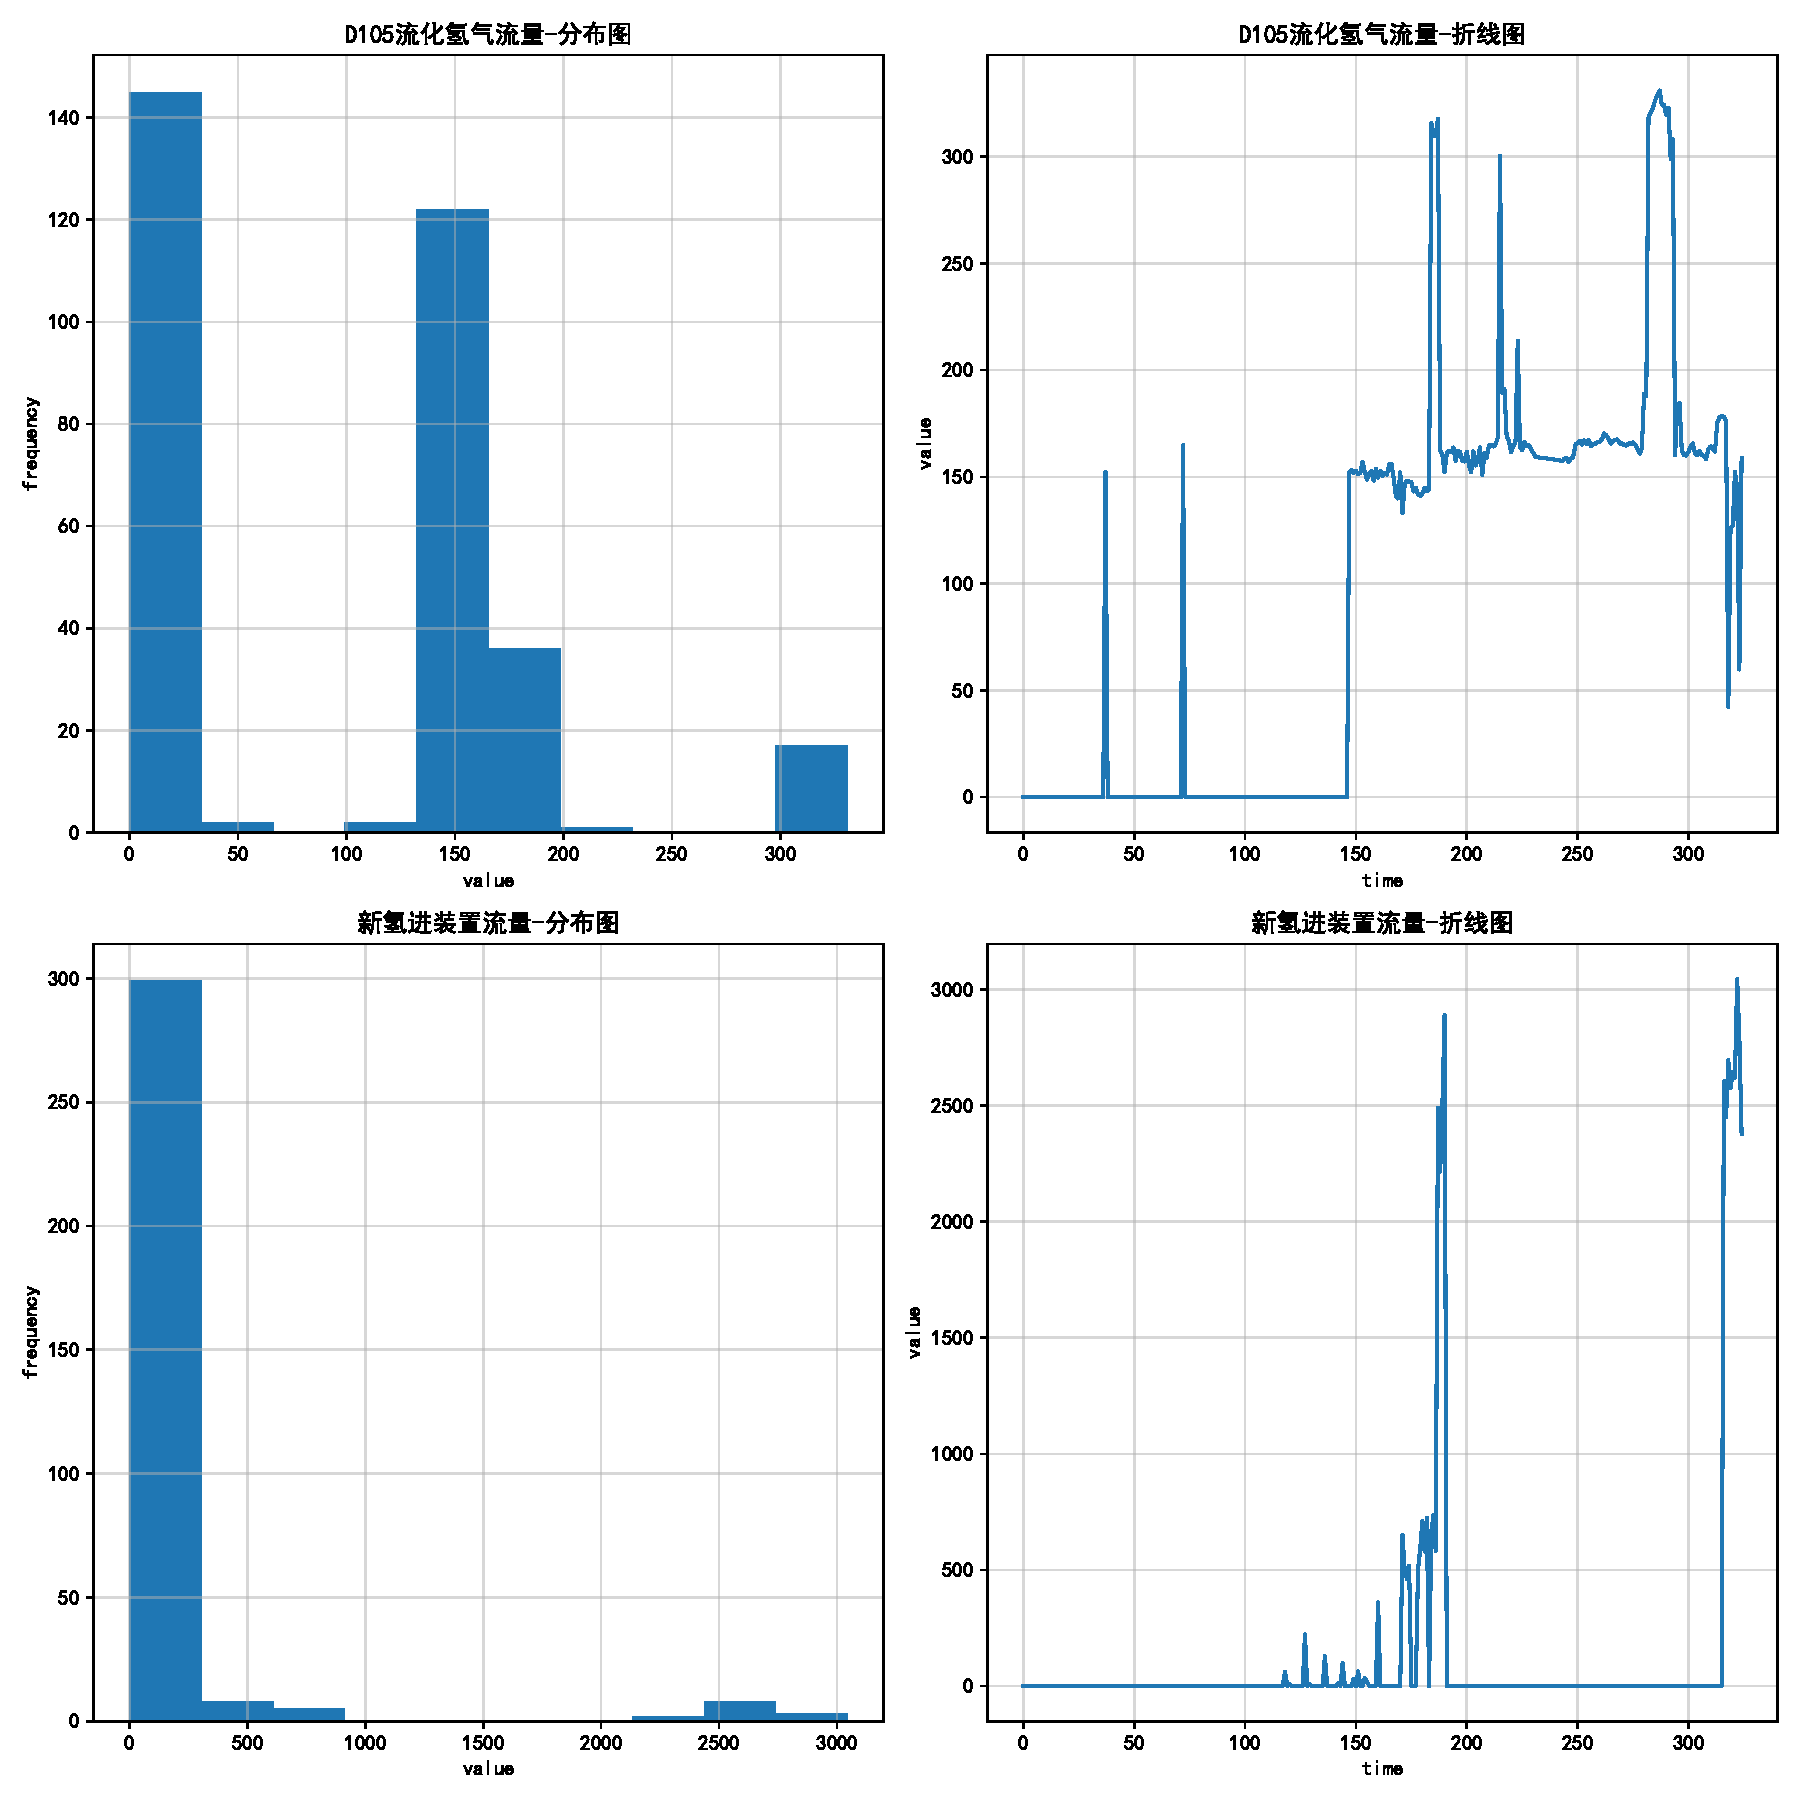
\includegraphics[width=0.32\textheight]{strategy-1}
		\subcaption{策略1}
	\end{minipage}
	\begin{minipage}[c]{0.4\textheight}
		\centering
		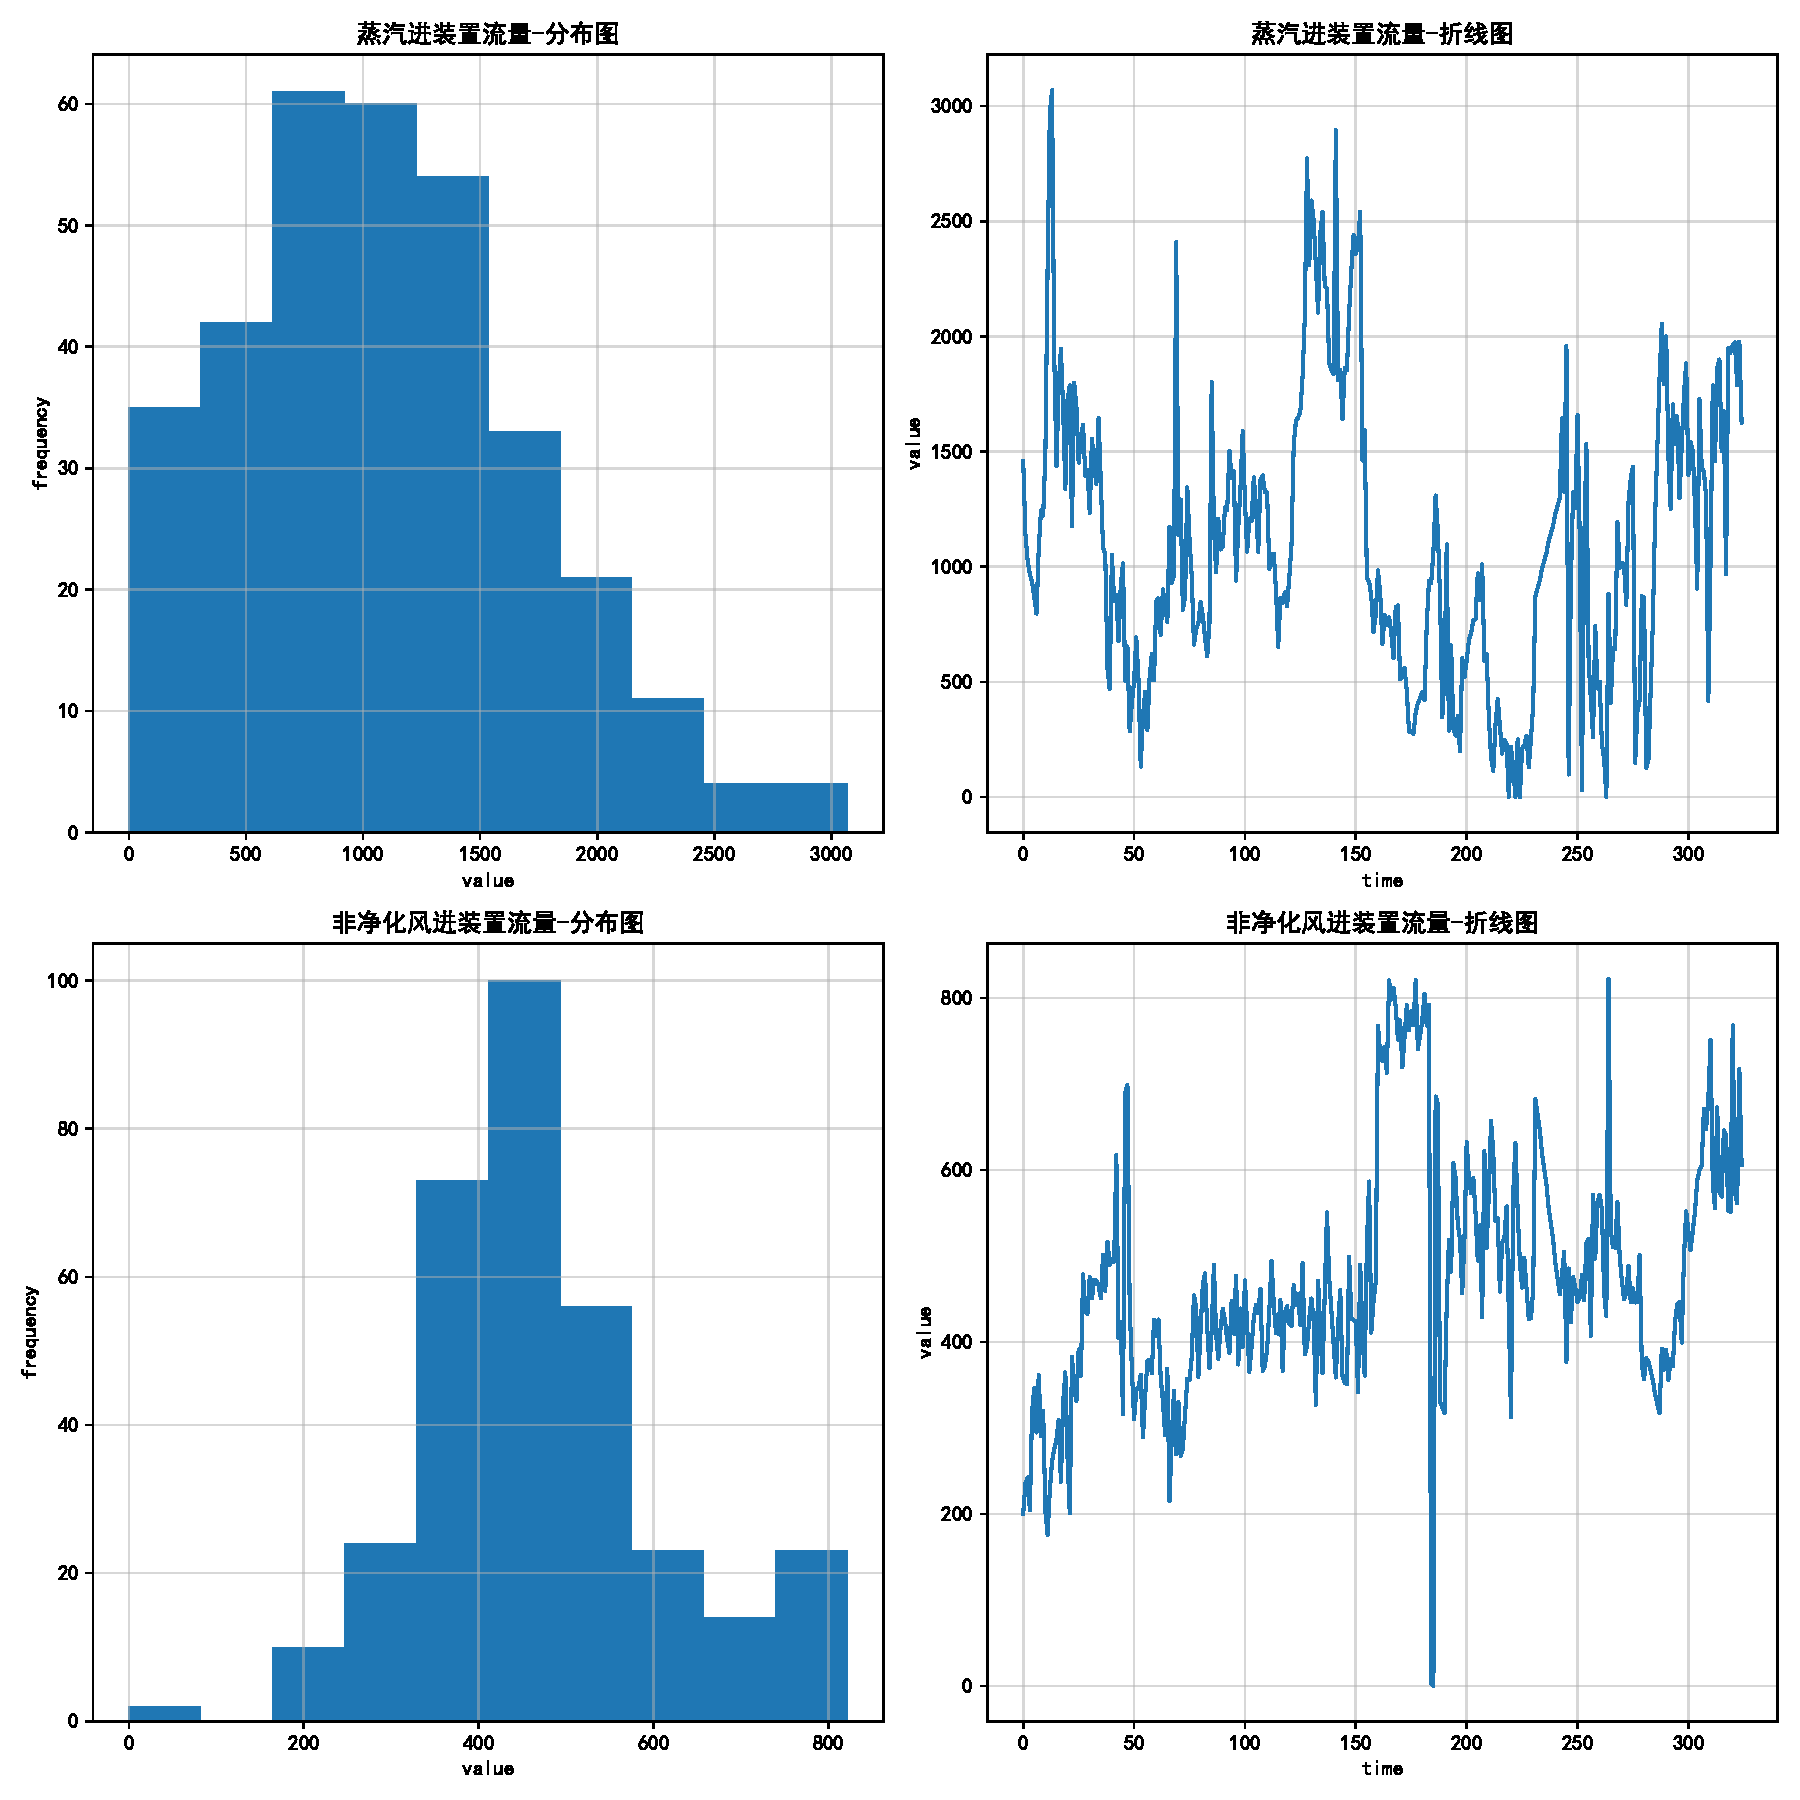
\includegraphics[width=0.32\textheight]{strategy-2}
		\subcaption{策略2}
	\end{minipage}
	\begin{minipage}[c]{0.4\textwidth}
		\centering
		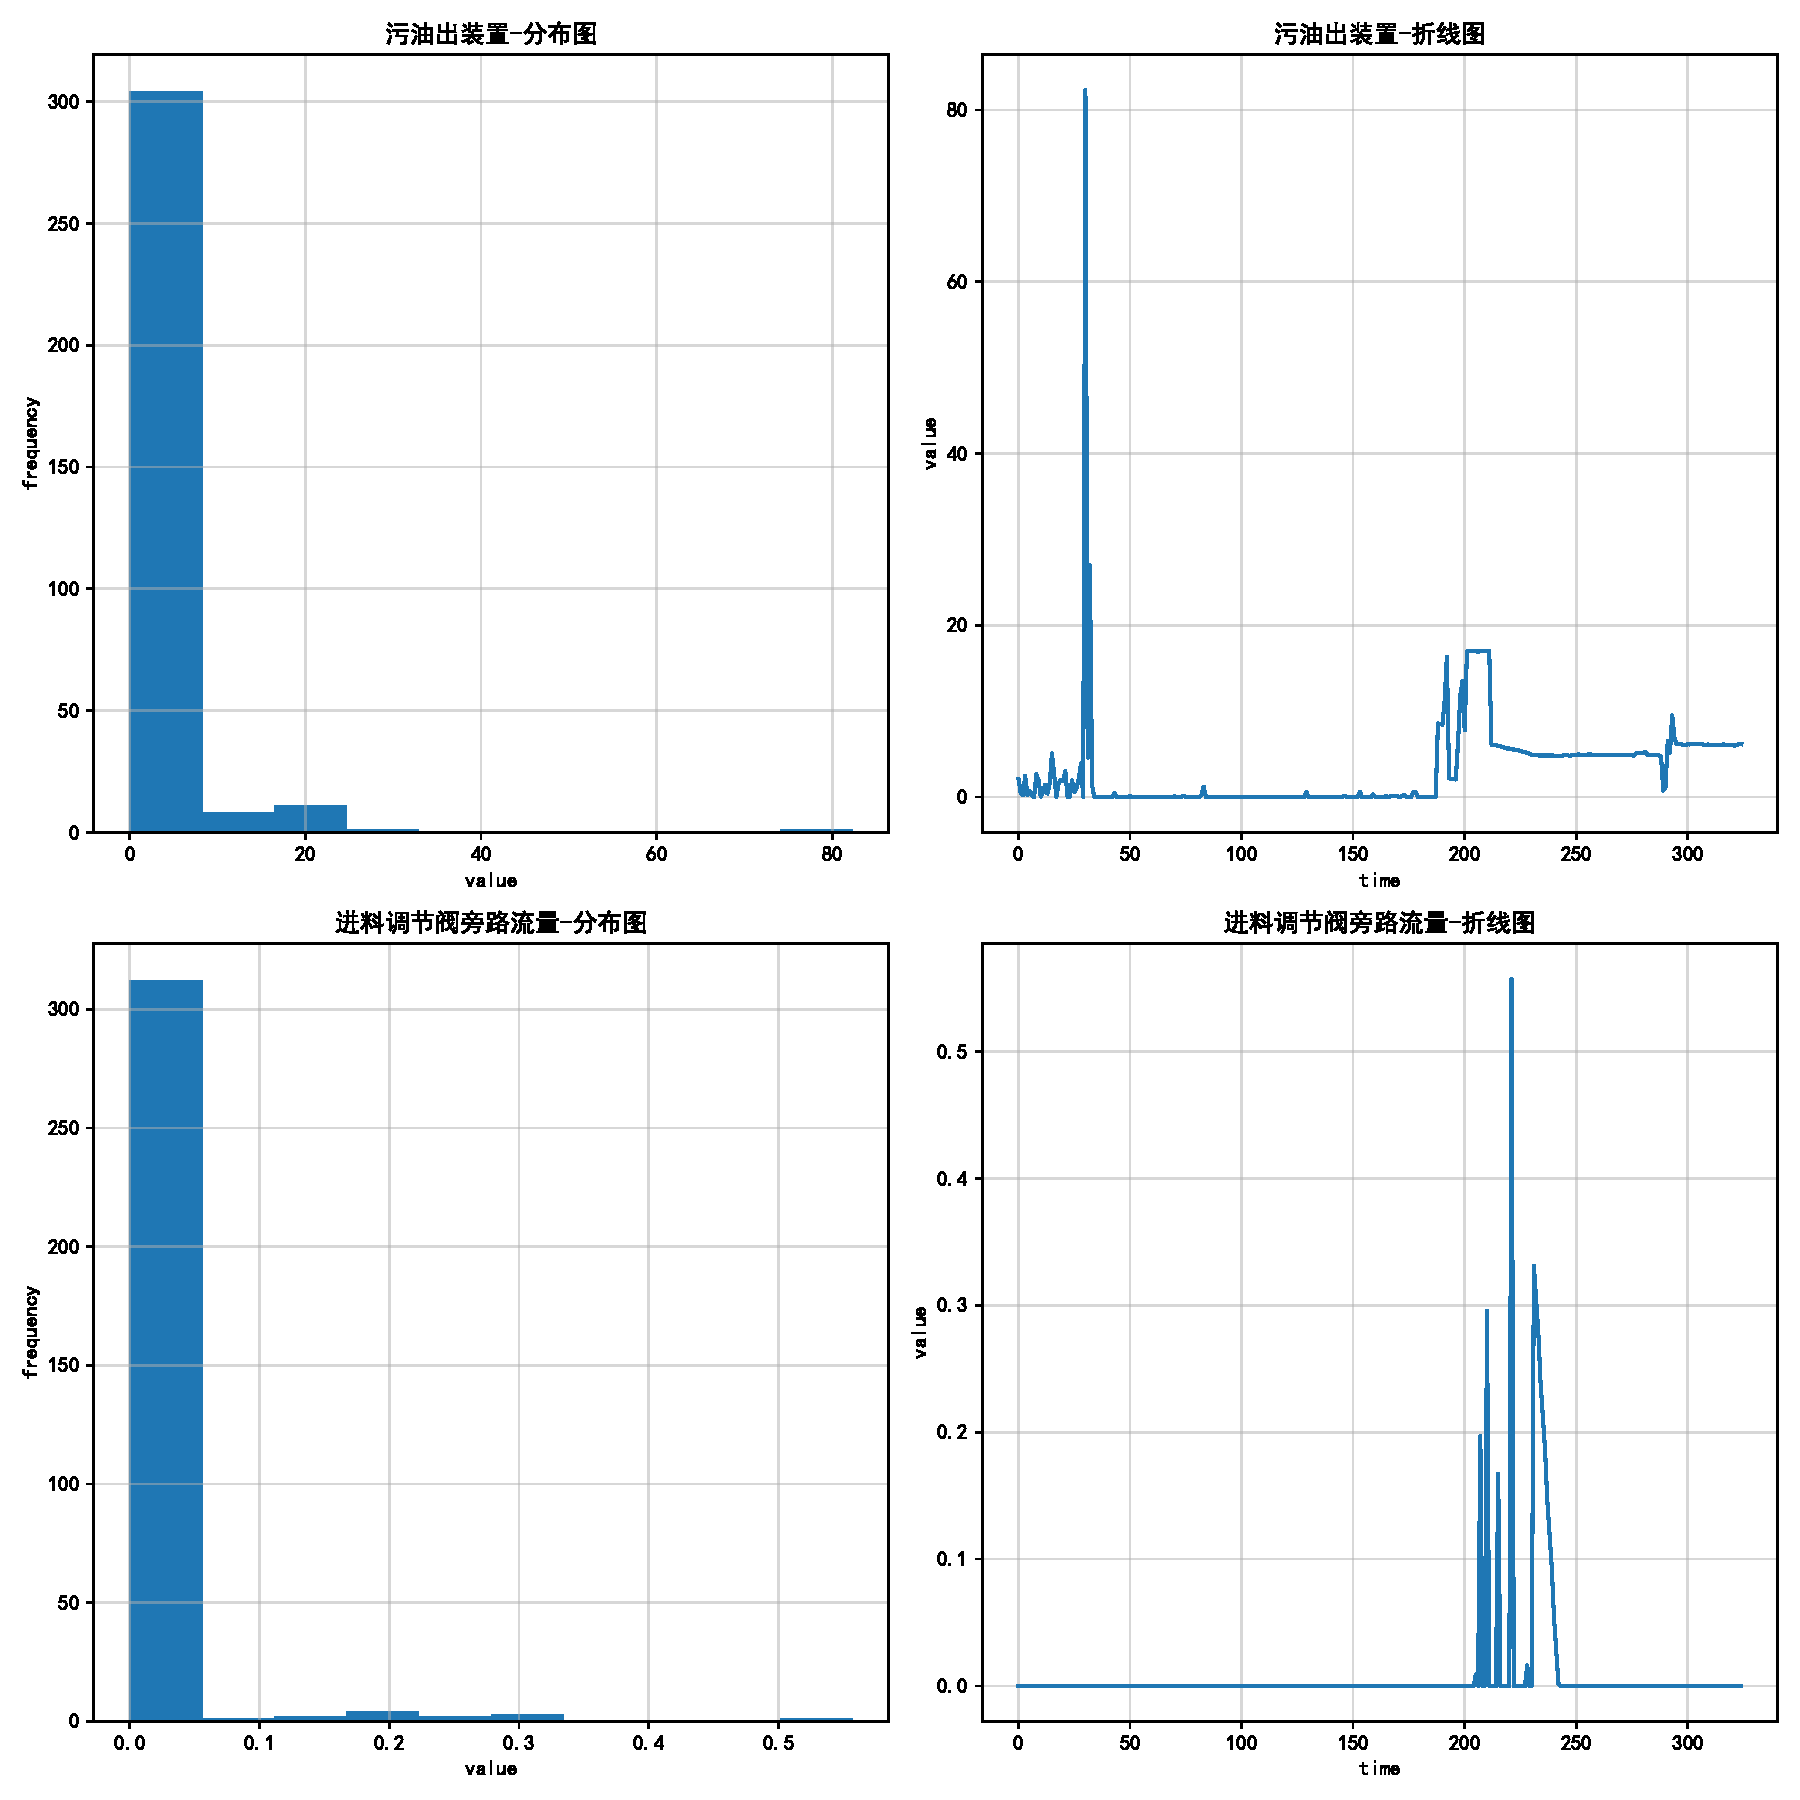
\includegraphics[width=0.32\textheight]{strategy-3}
		\subcaption{策略3}
	\end{minipage}
	\caption{3种处理空值的策略}
\end{figure}

对于策略2与\ref{sec:empty-analyze}中填充的$NaN$,用每列其余变量的均值代替,具体方法用的是\texttt{scikit-learn}的\texttt{impute.SimpleImpute} 。

\FloatBarrier
\subsection{问题二:寻找建模主要变量}
\FloatBarrier
\subsubsection{问题分析}

建立降低辛烷值损失模型涉及包括7个原料性质、2个待生吸附剂性质、2个再生吸附剂性质、2个产品性质等变量以及另外354个操作变量(共计367个变量),工程技术应用中经常使用先降维后建模的方法,这有利于忽略次要因素,发现并分析影响模型的主要变量与因素。

寻找主要变量的方法有两类,一类方法是主成分分析(Principal Component Analysis, PCA),其所要做的就是设法将原来众多
具有一定相关性的变量,重新组合为一组新的相互无关的综合变量来代替原来的
变量。通常,数学上的处理方法就是将原来的变量做线性组合,作为新的综合变
量。另一类方式是特征筛选,通过剔除无关变量与混淆变量,保留主要变量与关键变量,从而提升后续机器学习建模过程的表现。

在本题中,虽然PCA方法也能起到降维的作用,但考虑到问题3与问题4需要对主要变量进行优化,而不是PCA计算得到的主成分变量,所以决定在此使用特征筛选方法寻找建模主要变量。

在本题中,虽然有大量的特征可使用,有的特征携带的信息丰富,有的特征携带的信息有重叠,有的特征则属于无关特征,如果所有特征不经筛选地全部作为训练特征,经常会出现维度灾难问题,甚至会降低模型的准确性。因此,必须需要进行特征筛选,排除无效/冗余的特征,把有用的特征挑选出来作为模型的训练数据。



\FloatBarrier
\subsubsection{通过特征筛选获取主要变量}\label{sec:feature-selection}

特征筛选的方法又分为3类,分别是Filter方法(过滤式),Wrapper方法(封装式)和Embedded方法(嵌入式):

\begin{enumerate}
	\item 过滤式:主要思想是对每一维特征“打分”,即给每一维的特征赋予权重,这样的权重就代表着该特征的重要性,然后依据权重排序。主要方法有卡方检验(Chi--squared Test),信息增益(Information Gain),相关系数(Correlation Coefficient Scores)等方法。
	\item 封装式:主要思想是将子集的选择看作是一个搜索寻优问题,生成不同的组合,对组合进行评价,再与其他的组合进行比较。这样就将子集的选择看作是一个优化问题,这里有很多的优化算法可以解决,尤其是一些启发式的优化算法,如GA、PSO等。最为经典的代表是\texttt{scikit-learn}实现的递归特征消除法(Recursion Feature Elimination, RFE)
	\item 嵌入式:主要思想是在模型既定的情况下学习出对提高模型准确性最好的特征,也就是在确定模型的过程中,挑选出那些对模型的训练有重要意义的特征。主要方法有用带有L1正则化的项完成特征选择(也可以结合L2惩罚项来优化)、随机森林平均不纯度减少法/平均精确度减少法。
\end{enumerate}

经过实践,发现虽然过滤式虽然计算速度快,但是并不能准确地筛选出关键特征;封装式虽然筛选效果好,但是计算速度很慢;嵌入式的筛选效果与封装式基本持平,但计算速度相对快很多,故选择嵌入式特征筛选方法。

% 从这抄的 https://blog.csdn.net/yangxudong/article/details/53899260

GBDT模型能够在建模过程中计算各个特征的特征重要度。在GBDT模型中,特征$j$的全局重要度通过特征$j$在单颗树中的重要度的平均值来衡量: 
\begin{equation}\label{eq:gbdt-1}
	\hat{J^2_j} = \frac{1}{M} \sum^M_{m=1}\hat{J^2_j}(T_m)
\end{equation}

其中,$M$是树的数量。特征$j$在单颗树中的重要度的如下:

\begin{equation}\label{eq:gbdt-2}
	\hat{J^2_j} = \frac{1}{M} \sum^{L-1}_{t=1}\hat{i^2_t} I (v_t=j)
\end{equation}

其中, $L$ 为树的叶子节点数量,$L−1$ 即为树的非叶子节点数量(构建的树都是具有左右孩子的二叉树),$_t$ 是和节点t相关联的特征,$\hat{i^2_t}$是节点$t$分裂之后平方损失的减少值。

考虑到GBDT模型的准确性与鲁棒性优势,选用GBDT模型作为嵌入式特征筛选法的基模型。GBDT采用的是\texttt{sklearn.ensemble.GradientBoostingRegressor},嵌入式特征筛选采用的是\texttt{sklearn.feature\_selection.SelectFromModel}。

\begin{figure}[htb]
	\centering
	\begin{minipage}[c]{0.4\textwidth}
		\centering
		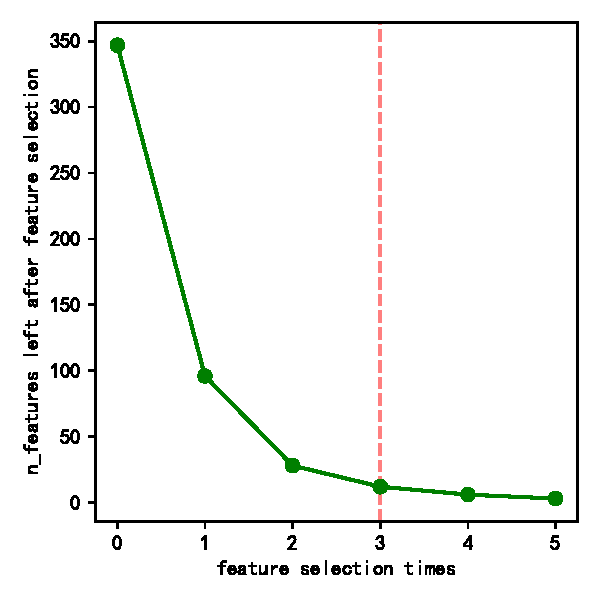
\includegraphics[width=0.32\textheight]{feature-selection-feats}
		\subcaption{特征筛选n次后剩余特征数}
	\end{minipage}
	\begin{minipage}[c]{0.4\textheight}
		\centering
		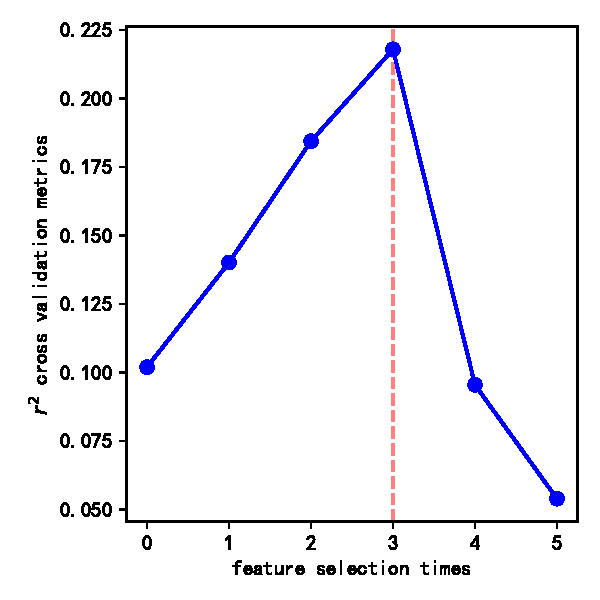
\includegraphics[width=0.32\textheight]{feature-selection-perfs}
		\subcaption{特征筛选次数与$r^2$评价指标的关系}
	\end{minipage}
	\caption{特征筛选n次后的剩余特征数与$r^2$评价指标}
\end{figure}

考虑到一次特征筛选可能并不能得到最好的筛选效果(无关变量还混杂在剩余的变量中),于是在本次建模过程中队员们通过多次试验实验探索了特征筛选次数与剩余特征数、下游模型$r^2$的关系。下游模型与章节\ref{sec:modeling}一致,为LightGBM模型。我们将特征筛选器与回归器组合成一个pipeline: \texttt{Pipeline(SelectFromModel, LGBMRegressor)},作为一个整体来验证特征筛选的效果。

该实验分别进行了0次特征筛选到5次特征筛选(0次特征筛选表示不进行特征筛选),得到的实验结果如图4和表\ref{tab:002}所示。

实验反映了剩余特征数的下降程度随着特征筛选次数的增加逐渐减小,而模型整体表现在特征筛选数为3时到达峰值,之后迅速下降,说明3次特征筛选后保留的均为重要特征,如果再删除就会极大地影响模型表现。

\begin{table}[!htbp]
	\caption{特征筛选n次后的各指标}\label{tab:002} \centering
	\begin{tabular}{ccc}
		\toprule[1.5pt]
	feature selection times &  $r^2$ metrics &  n\_features left \\
		\midrule[1pt]
           0 &       0.101955 &              347 \\
			1 &       0.140157 &               96 \\
			2 &       0.184434 &               28 \\
			3 &       0.217998 &               12 \\
			4 &       0.095470 &                6 \\
			5 &       0.053913 &                3 \\
		\bottomrule[1.5pt]
	\end{tabular}
\end{table}

通过实验,确定了做3次特征筛选的方案。根据这一方案,筛选出了12个主要变量,变量的名称与特征重要度见图5与表\ref{tab:003}。

\begin{table}[htb]
	\caption{主要变量的特征重要度}\label{tab:003} \centering
	\begin{tabular}{ccccc}
		\toprule[1.5pt]
		rank & feature importances & percentage (\%) &           name \\
		\midrule[1pt]
		0 &              0.0785 &          12.83 &   P-101B入口过滤器差压 \\
		1 &              0.0774 &          12.66 &      D101原料缓冲罐压力 \\
		2 &              0.0602 &           9.84 &         稳定塔下部温度 \\
		3 &              0.0596 &           9.74 &        D-204液位 \\
		4 &              0.0515 &           8.42 &    E-101D壳程出口管温度 \\
		5 &              0.0474 &           7.75 &          D-102温度 \\
		6 &              0.0443 &           7.25 &         精制汽油出装置温度 \\
		7 &              0.0408 &           6.67 &   F-101出口支管\#4温度 \\
		8 &              0.0390 &           6.37 &     R-101下部床层压降 \\
		9 &              0.0385 &           6.29 &       加热炉主火嘴瓦斯入口压力 \\
		10 &              0.0379 &           6.20 &       精制汽油出装置硫含量 \\
		11 &              0.0364 &           5.95 &           辛烷值 \\
		\bottomrule[1.5pt]
	\end{tabular}
\end{table}



\begin{figure}[htb]
	\centering
	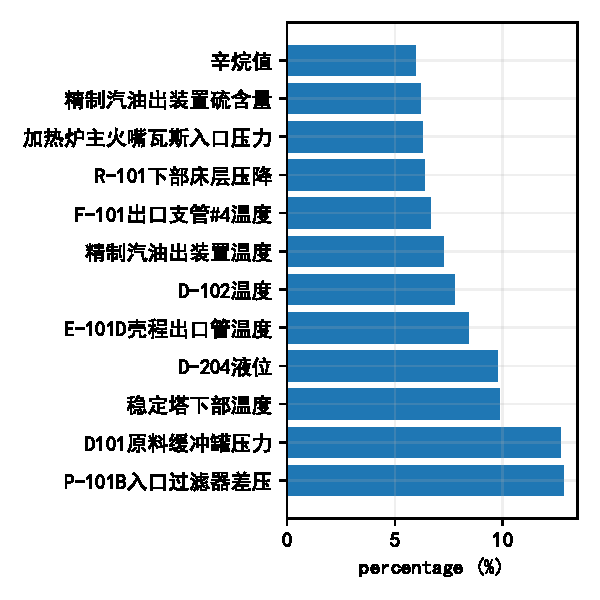
\includegraphics[width=.5\textwidth]{feat-imp}
	\caption{主要变量的特征重要度}
\end{figure}


\FloatBarrier
\subsubsection{主要变量数据分析}



对于筛选得到的12个主要变量,依据特征重要度取前4个变量加上预测目标RON损失一起做一个相关性分析,得到了图6所示的相关性矩阵图。根据pearson相关系数公式\eqref{eq:pearson}计算了12个主要变量加上RON损失两两之间的相关系数,并绘制了图7所示的特征相关系数热力图。

\begin{equation}\label{eq:pearson}
	\rho_{X,Y}=\frac{X,Y}{\sigma_X\sigma_Y}
\end{equation}


\begin{figure}[htb]
	\centering
	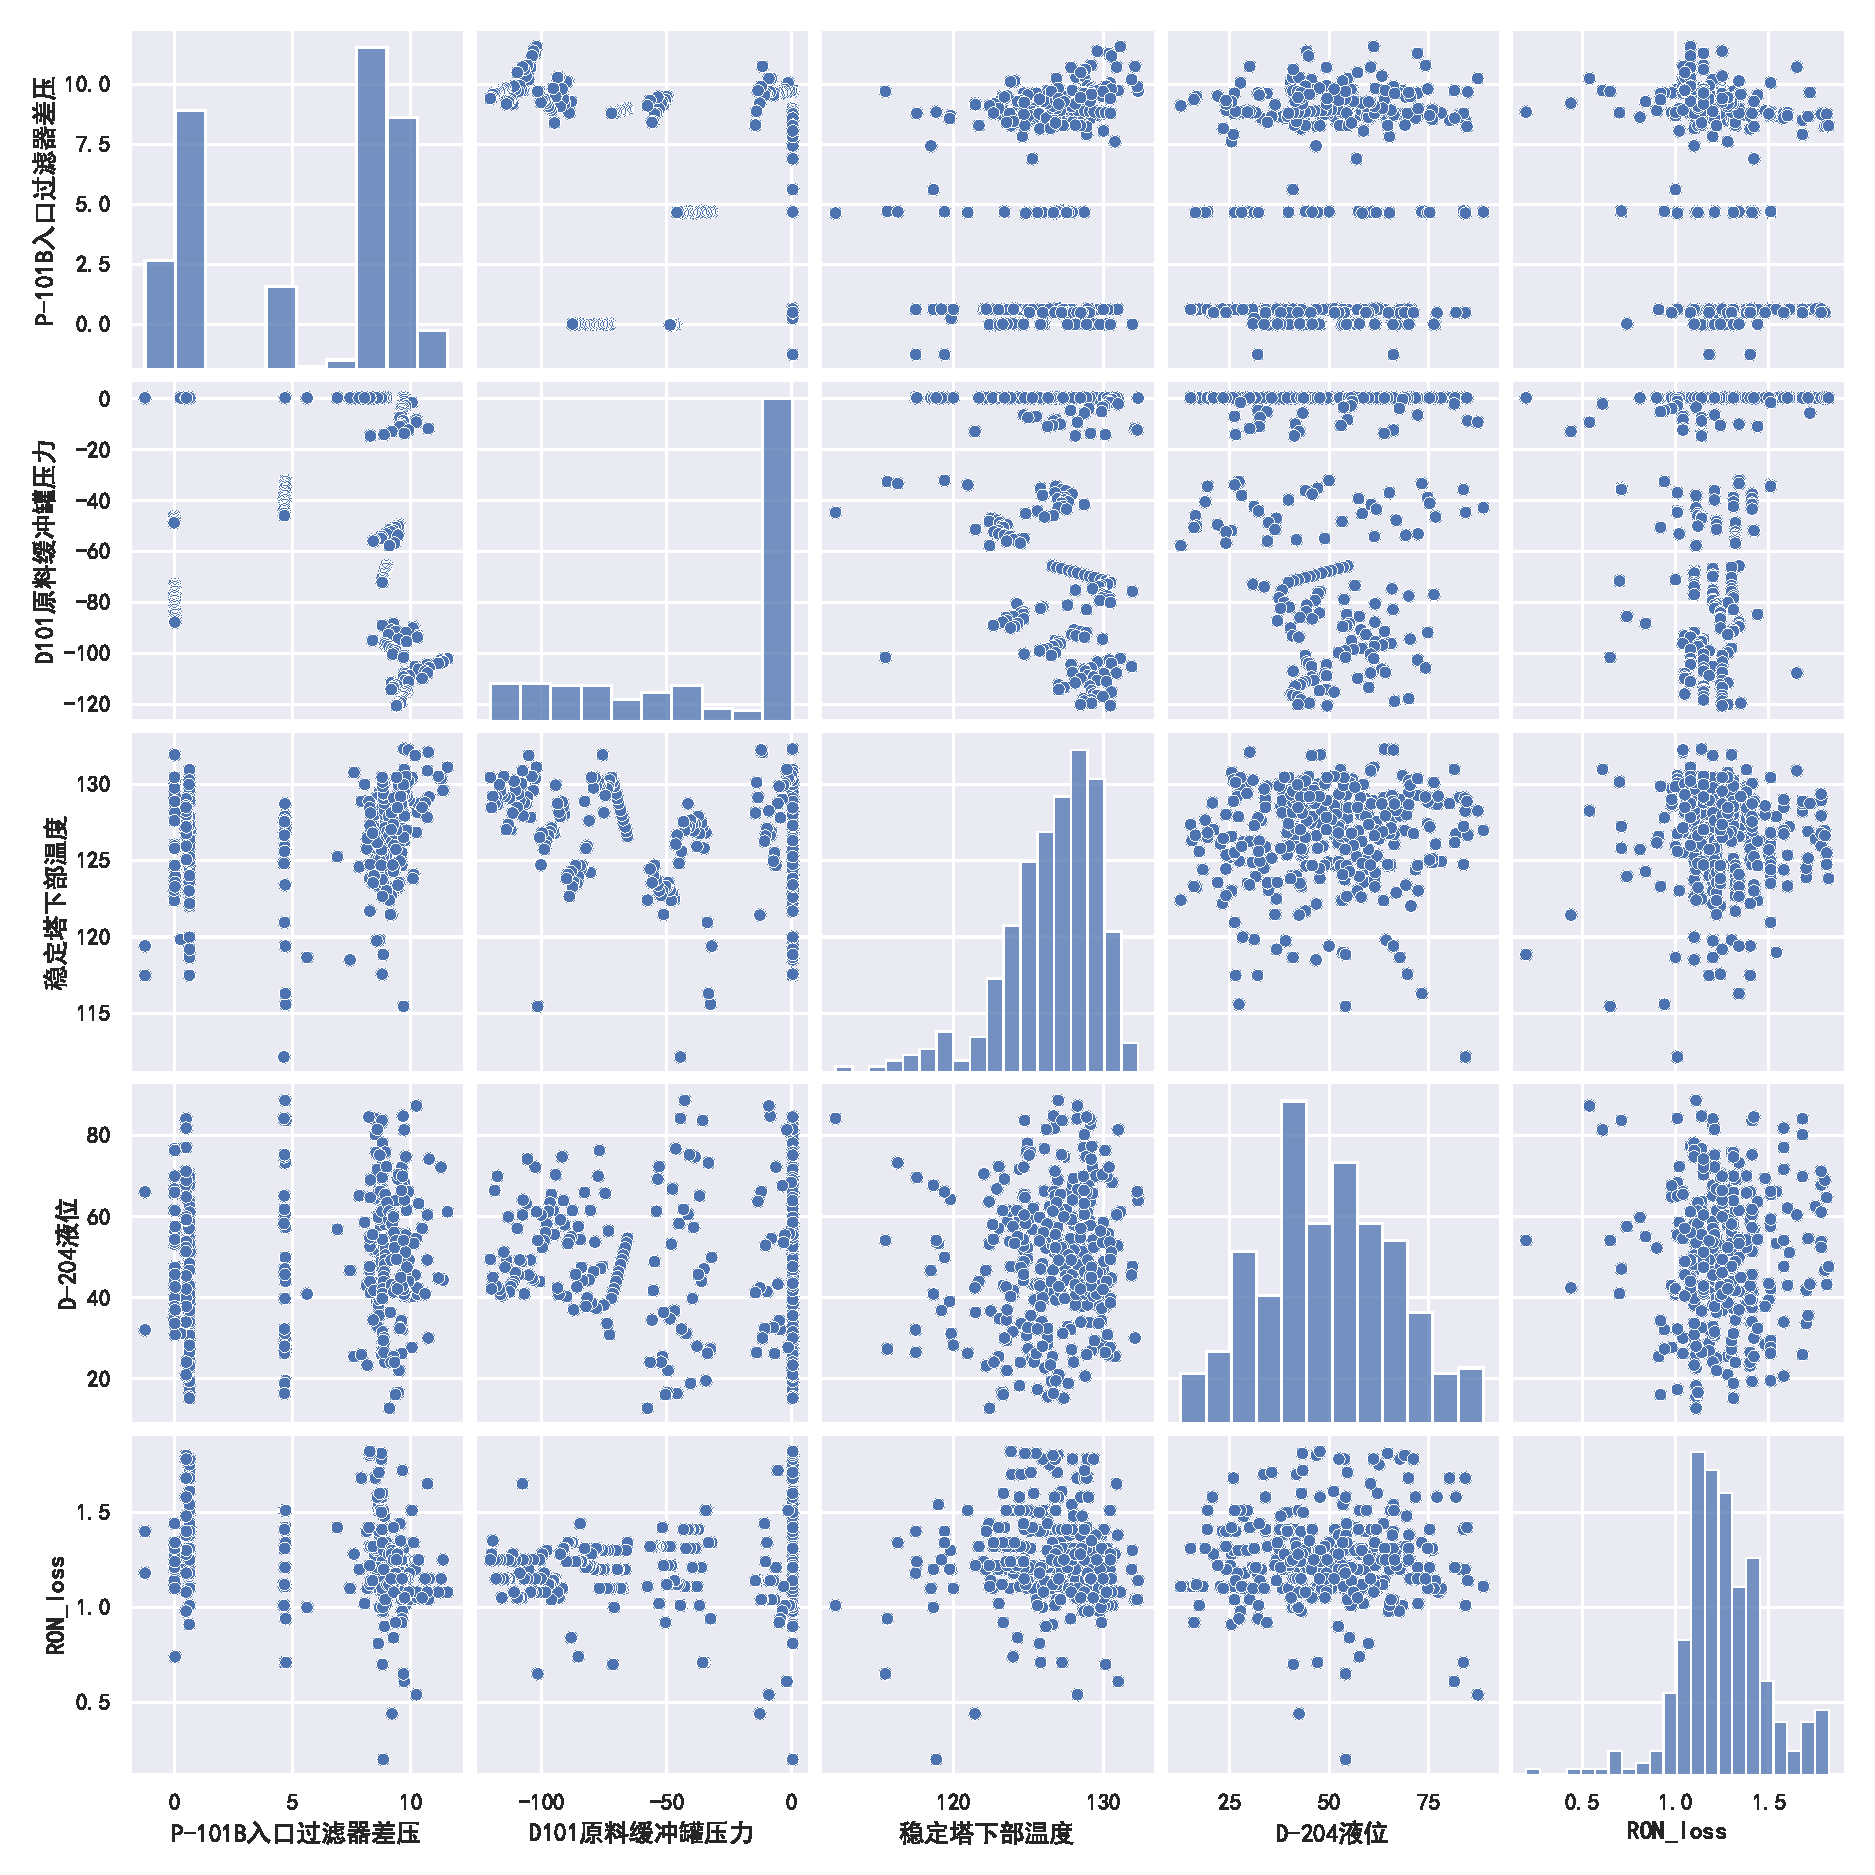
\includegraphics[width=1\textwidth]{pairplot}
	\caption{相关性矩阵图}
\end{figure}

\begin{figure}[htb]
	\centering
	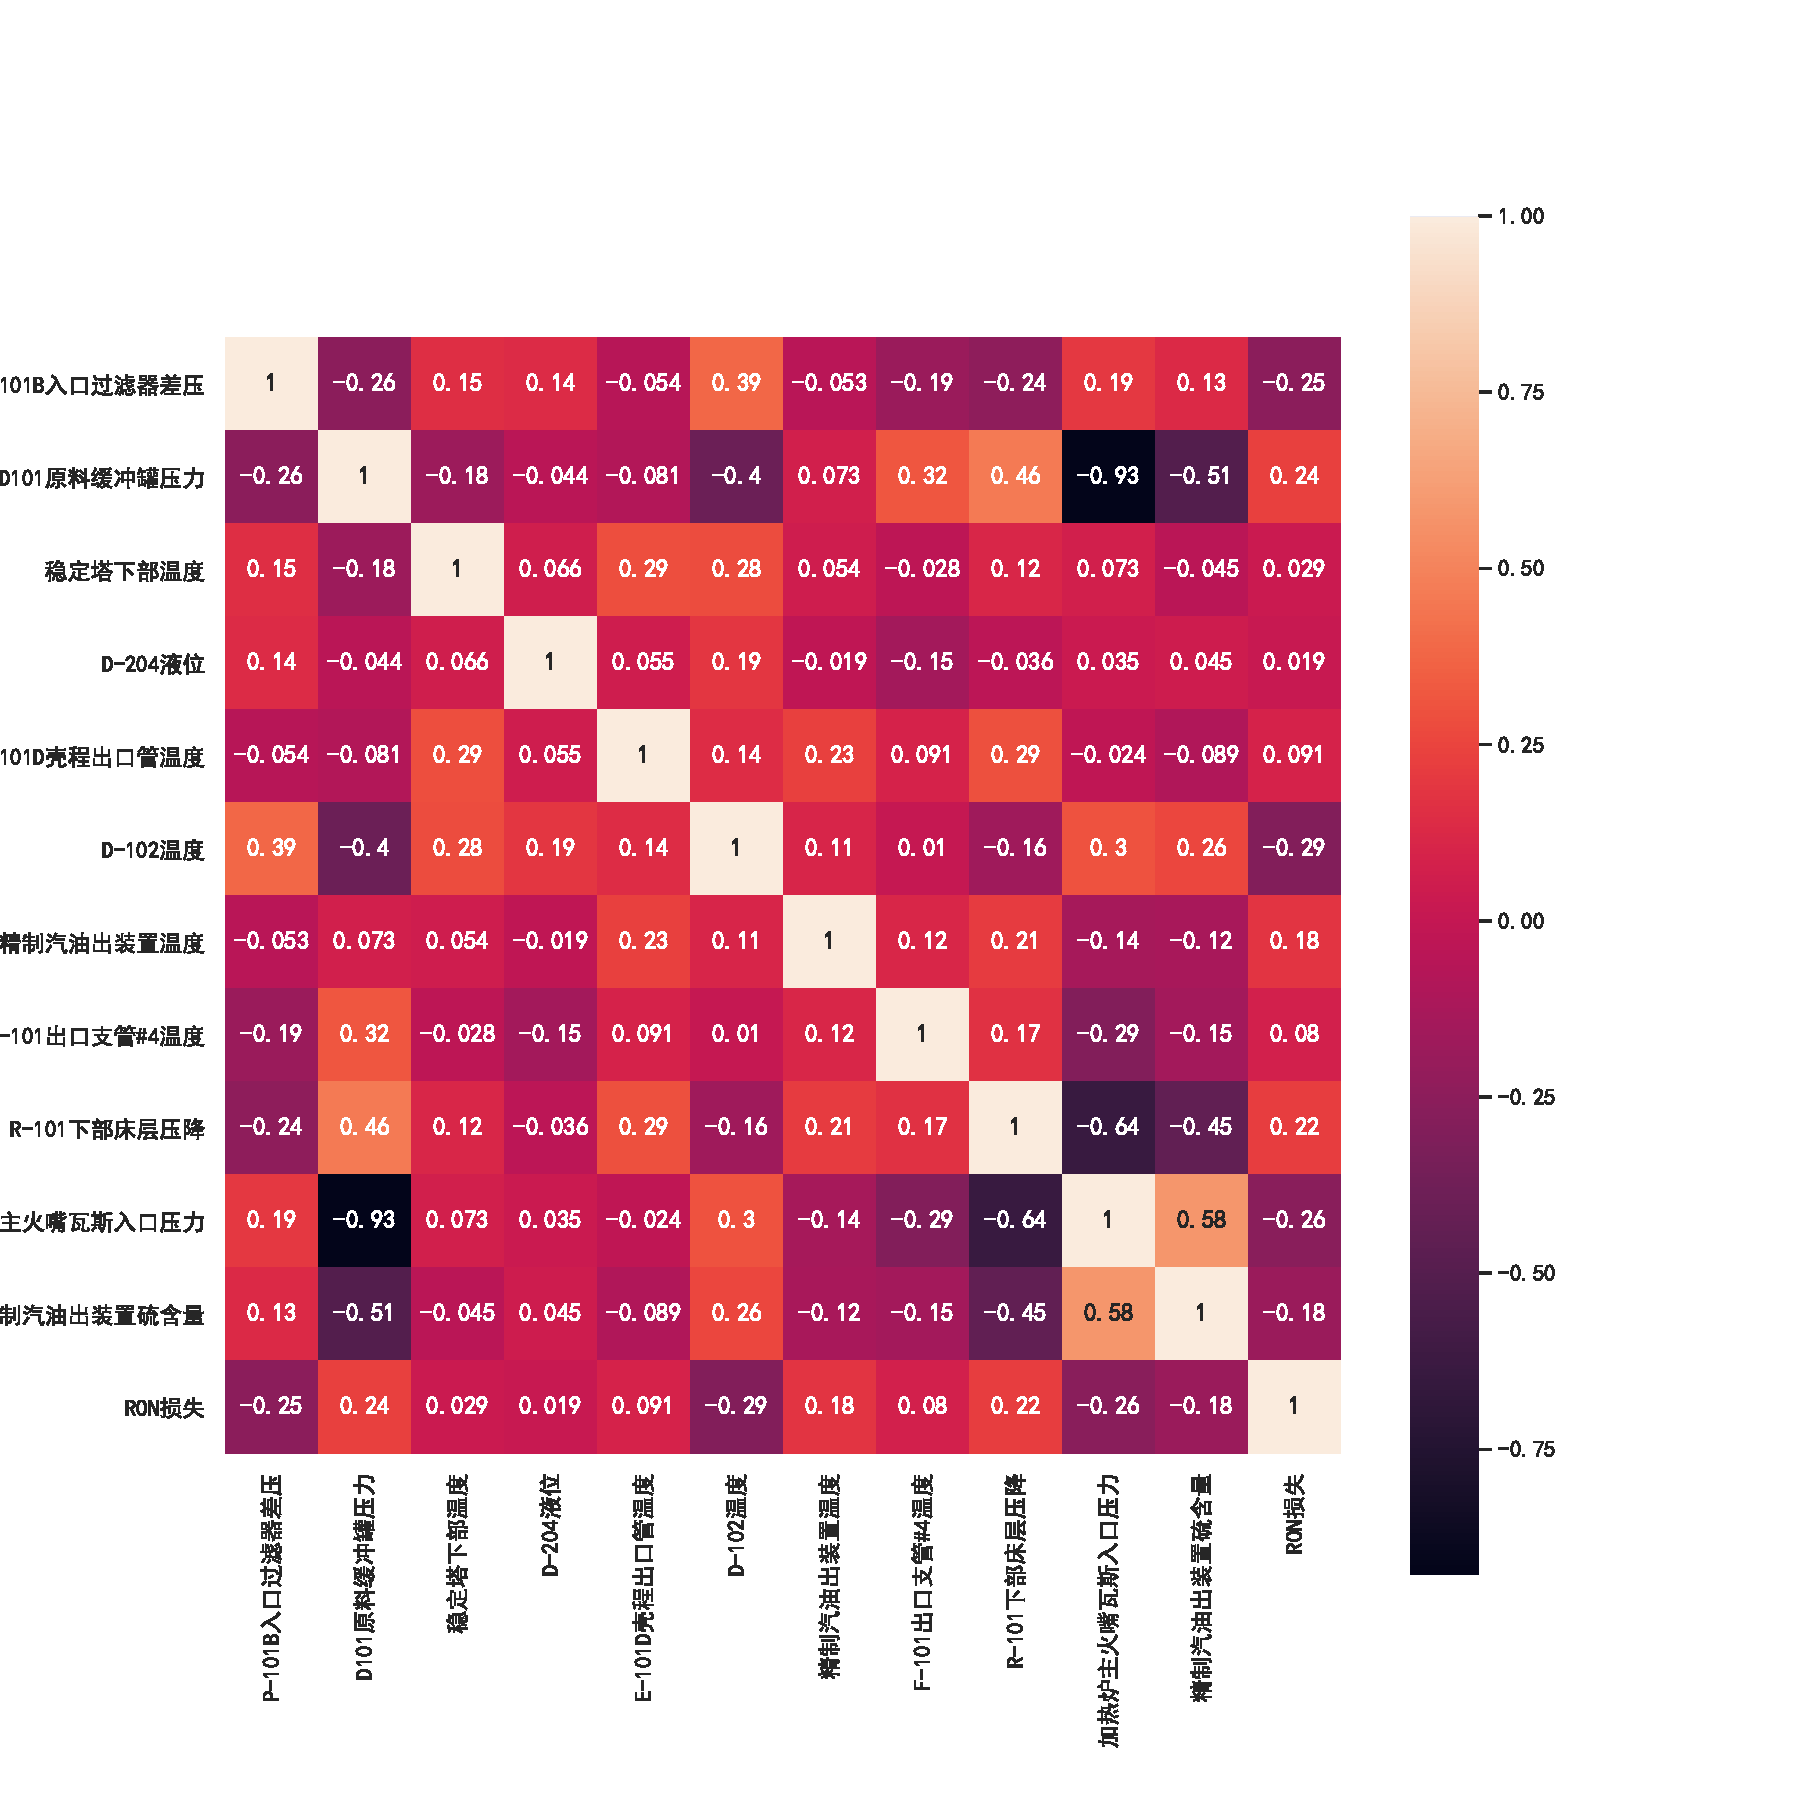
\includegraphics[width=1.2\textwidth]{heatmap}
	\caption{特征相关系数热力图}
\end{figure}



\FloatBarrier
\subsection{问题三:建立辛烷值(RON)损失预测模型}\label{sec:modeling}

\FloatBarrier
\subsubsection{问题分析}

本问题需要基于上述问题2找到的主要变量,通过数据挖掘技术建立辛烷值损失预测模型,并进行模型验证。

预测问题的本质是构造或学习获得问题输入与输出间的映射函数$f: \mathbb{R}^n \rightarrow \mathbb{R}$,常见解决思路有回归分析、灰色预测模型、神经网络等多种方法。而辛烷值损失预测问题由于操作变量复杂、采样误差较大等多种因素的影响,使得上述映射函数变为十分复杂的函数,实际上难以用化工理论和经验模型等传统方法或者简单的线性模型准确拟合。综上考虑,需要选用能处理特征与特征,特征与类别之间高度非线性和相互强耦联的关系的机器学习模型。通过对各种机器学习模型的反复试验,选择了LightGBM作为回归器。

\textbf{实验设计}

本实验的实验数据采用章节\ref{sec:data-process}处理得到的$325 \times 347$的数据。实验目标是结合章节\ref{sec:feature-selection}得到的特征筛选器,设计一个机器学习管线(详见\textbf{模型设计}),并通过5折交叉验证(5-folds Cross Validation, 5CV)的方式,在$r^2$评价指标下表现最好。

\begin{equation}\label{eq:r2}
	r^2=1-\frac{\sum_i^N(\hat{y^{(i)}}-y^{(i)})^2}{\sum_i^N(\bar{y}-y^{(i)})^2}
\end{equation}

$r^2$ 的计算方法见公式\eqref{eq:r2},其中$\sum_i^N(\bar{y}-y^{(i)})^2$表示使用预测产生的错误,是baseline,其中$\sum_i^N(\hat{y^{(i)}}-y^{(i)})^2$表示使用待验证模型才生的错误。$r^2$的取值范围为$(-\inf, 1]$,应该越大越好。


\textbf{模型设计}


考虑到所选特征的取值范围差异较大,如“加热炉主火嘴瓦斯入口压力”的取值范围是$[0.05, 0]$,“R-101下部床层压降”的取值范围是$[0, 120]$,容易造成不同尺度特征间难以比较的问题。缩放可以有效地解决上述问题,让变量之间可比性增强。除了特征之间尺度不同,特征的异常值与非正常分布也会对模型的鲁棒性与泛化能力造成影响。

QuantileTransformer 可以把每个特征转换到0-1均匀分布或者$\mathbb{N}(0,1)$的正态分布中。它执行的转换可以平滑掉非正常的分布,所以受到奇异点的影响比传统的StandardScaler要少。


根据章节\ref{sec:feature-selection}得到的特征筛选器,与上述的QuantileTransformer,组建了如图\ref{img:ml-pipeline}的机器学习管线。

\begin{figure}[htb]
	\centering
	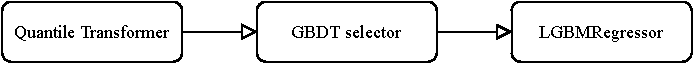
\includegraphics[width=.7\textwidth]{ml-pipeline}
	\caption{机器学习管线图}
	\label{img:ml-pipeline}
\end{figure}

该机器学习管线的处理流程为:先用QuantileTransformer将数据的分布进行转换,转换为者$\mathbb{N}(0,1)$的正态分布。然后用GBDT selector筛选出章节\ref{sec:feature-selection}得到的12个关键特征,最后用LGBMRegressor对筛选后的数据进行训练。

\FloatBarrier
\subsubsection{模型训练与验证}

通过上文初步建立的模型,对实验数据进行训练与验证得到的$r^2$=0.2179,其效果不能满足预期。经过分析,认为实验数据含有部分异常样本,需要将这些异常样本从实验数据中甄别并剔除。

检测异常样本的方法是用实验数据对机器学习管线进行训练,并在原数据上进行预测,并用的公式的方法\ref{eq:err}计算误差,如果误差大于阈值$E_t$,则认为是异常样本。

\begin{equation}\label{eq:err}
	E=|y-\hat{y}|
\end{equation}


\begin{figure}[htb]
	\centering
	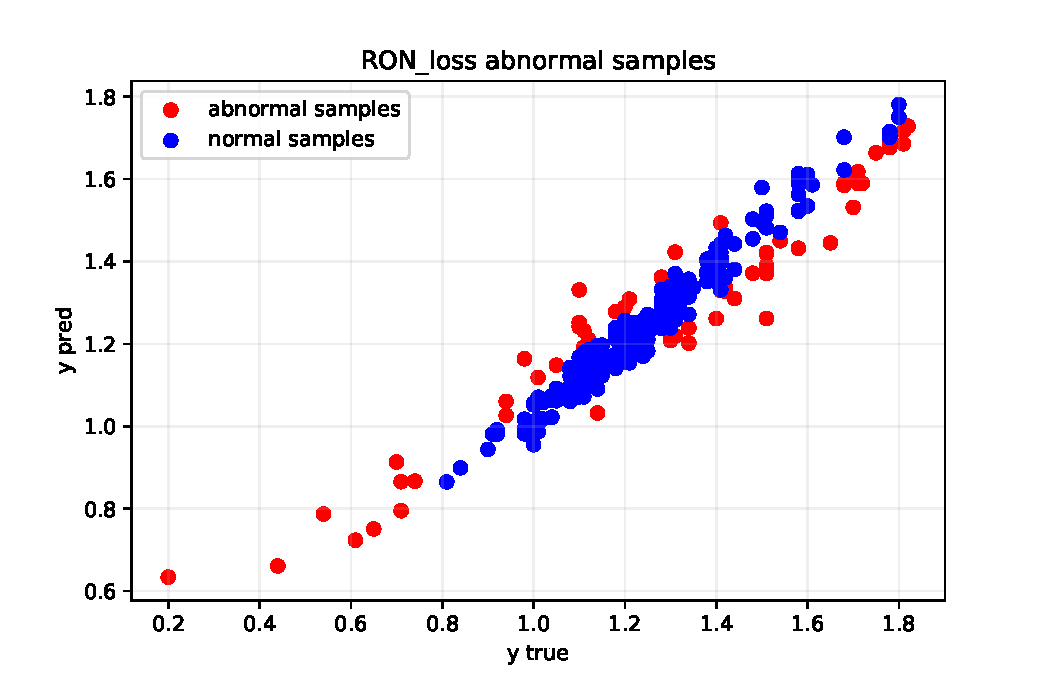
\includegraphics[width=.7\textwidth]{RON-loss-abnormal}
	\caption{删除异常样本}
	\label{img:abnormal}
\end{figure}

经过多次实验,确定阈值$E_t$=0.08,在该阈值下删除了60个样本。实验结果如图\ref{img:abnormal}所示。

删除异常样本后,在5CV下$r^2$=0.3727,说明原实验数据受异常样本影响较大,删除异常样本后模型能达到不错的效果。

最后用5CV方法划分了5个不同的训练集与验证集,进行了综合地评估,在5次验证中验证集的$r^2$评价指标分别为0.477, 0.409, 0.289, 0.362, 0.324,均值为0.3727,模型表现稳定,具有鲁棒性与泛化能力。在训练集上$r^2$评价指标为0.911,pearson相关系数为0.9648,见图\ref{RON-loss-cv}。

\begin{figure}[htb]
	\centering
	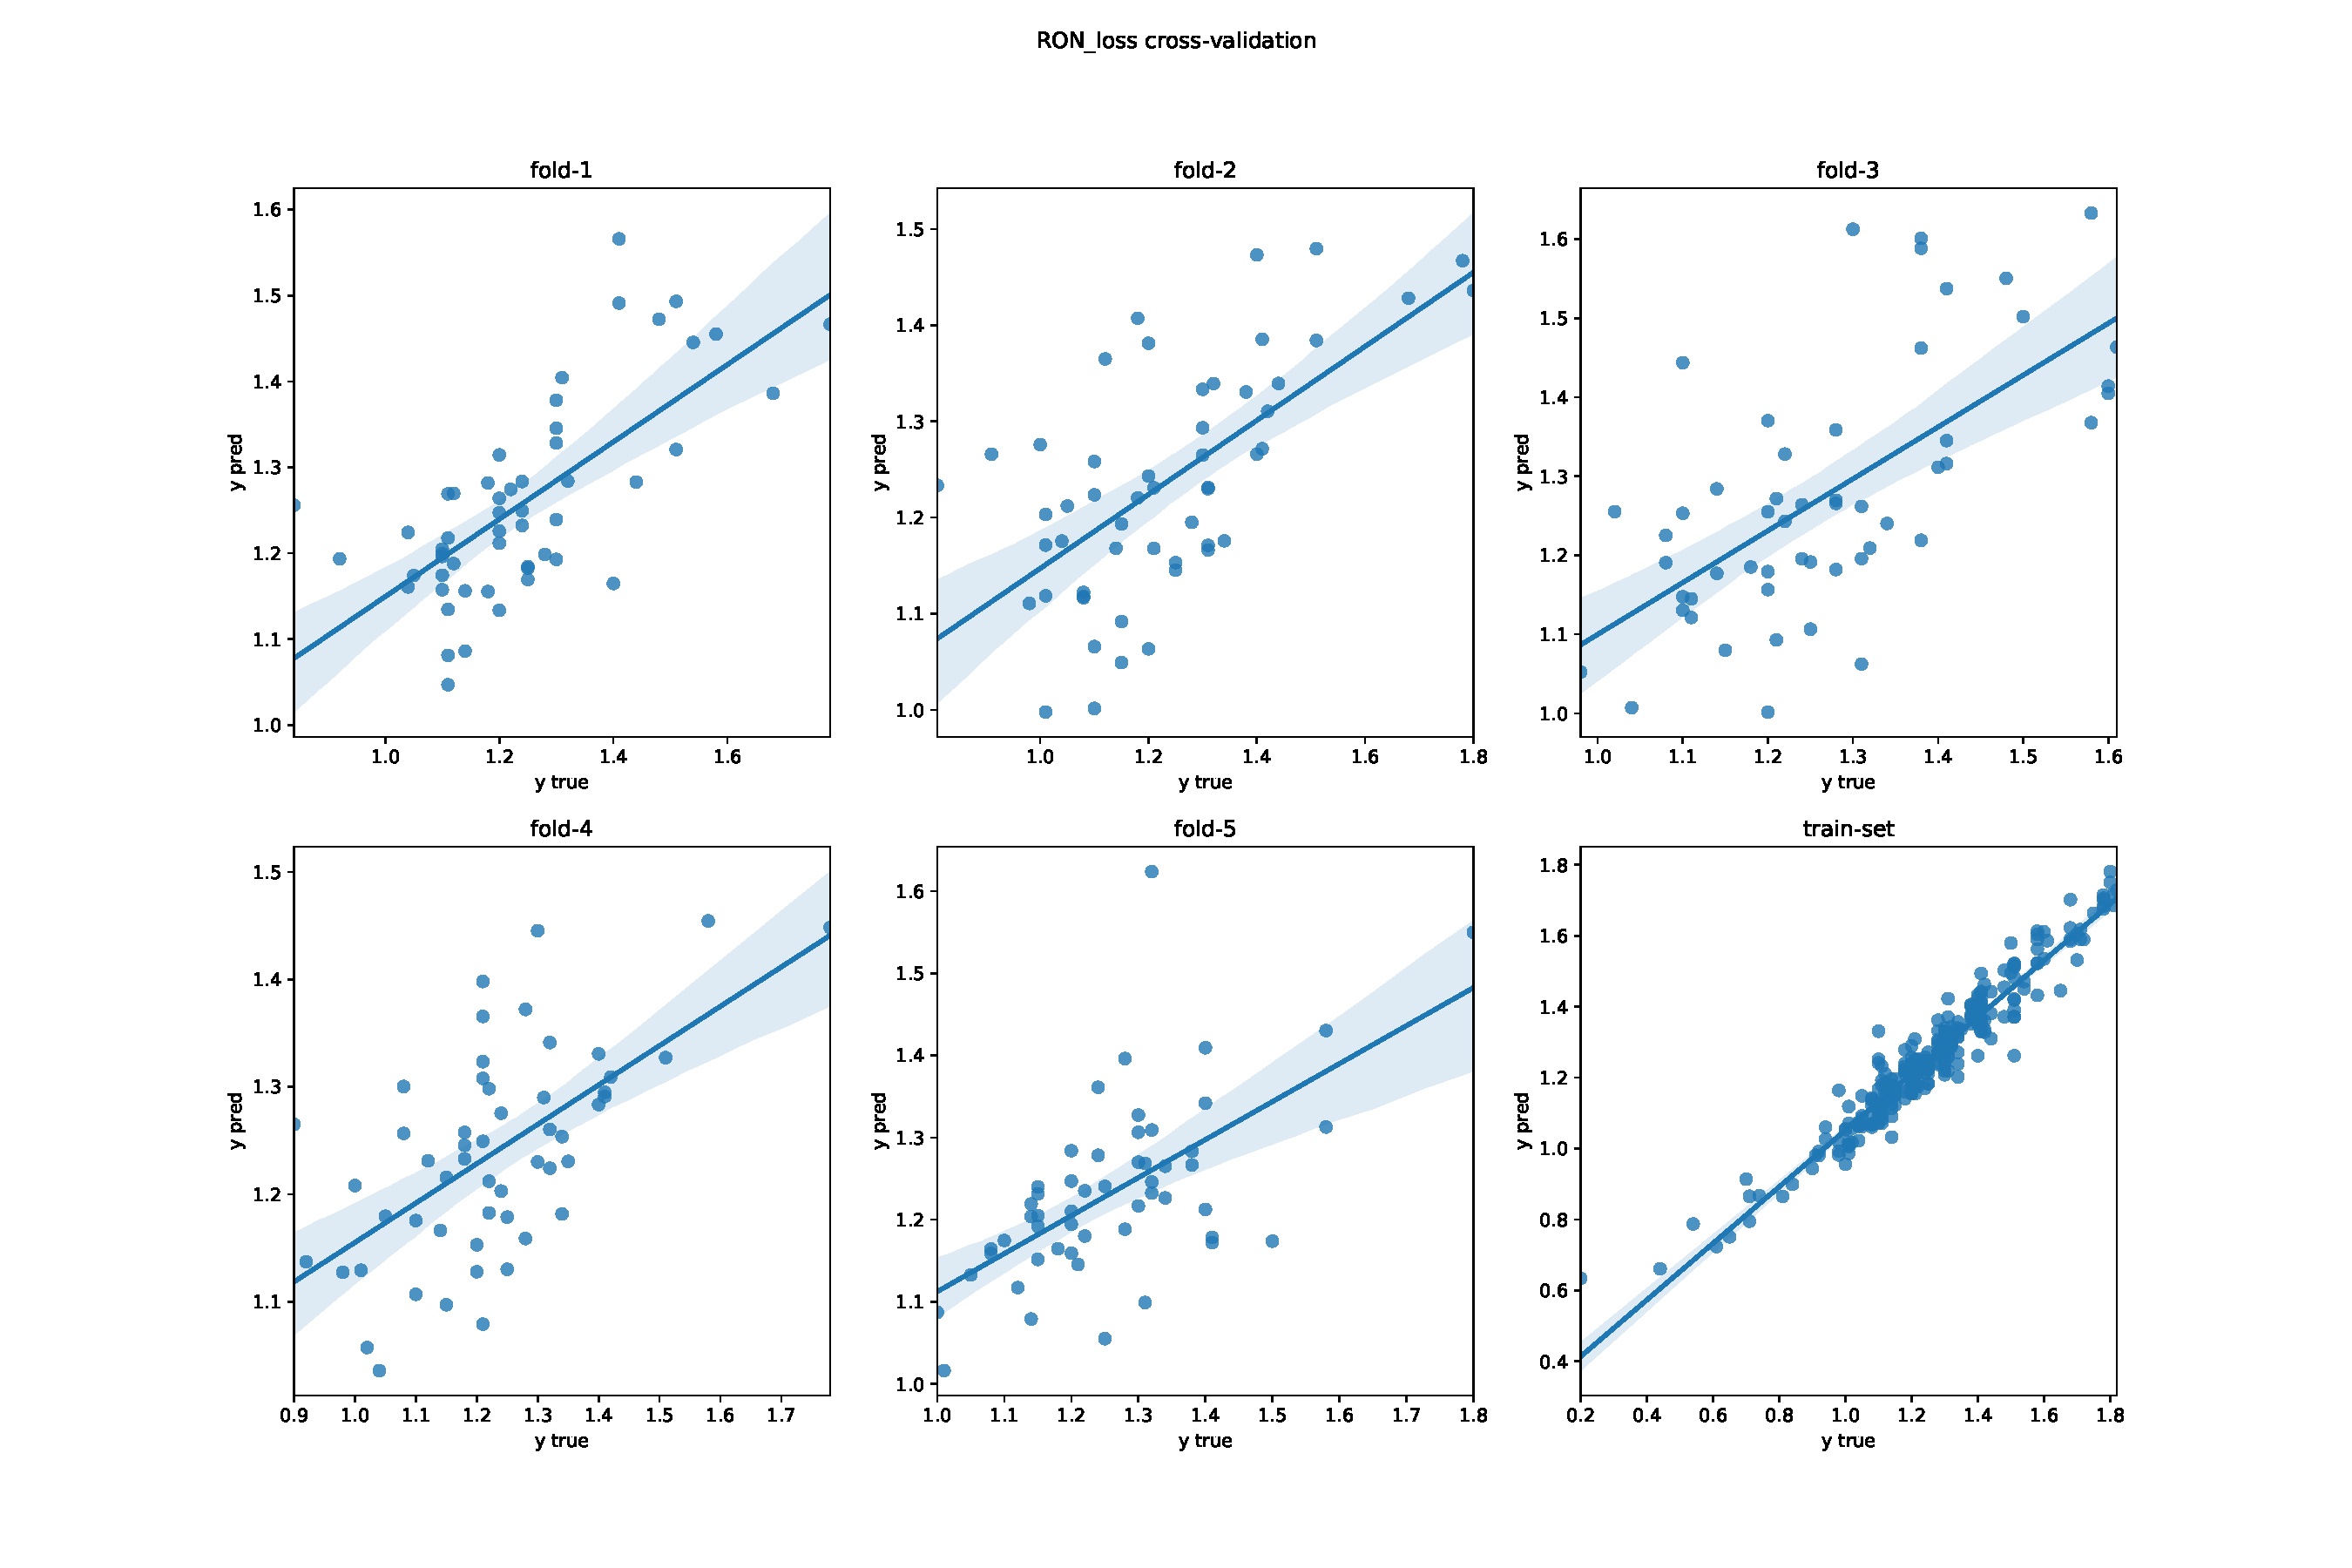
\includegraphics[width=1\textwidth]{RON-loss-cross-validation}
	\caption{对RON损失进行交叉验证}
	\label{RON-loss-cv}
\end{figure}



\FloatBarrier
\subsection{问题四:主要变量操作方案的优化}

\FloatBarrier
\subsubsection{问题分析}\label{sec:opt-problem-analyze}


问题四的目标是在保证产品硫含量不大于5$\mu$/g的前提下,将章节\ref{sec:modeling}得到的RON损失模型作为评价函数,对章节\ref{sec:feature-selection}得到的12个主要变量(其中11个变量是操作条件,原料的RON值是常数)进行优化,尽量使RON损失降幅超过30\%。

%\begin{fig\textit{ure}[htb]
%	\centering
%	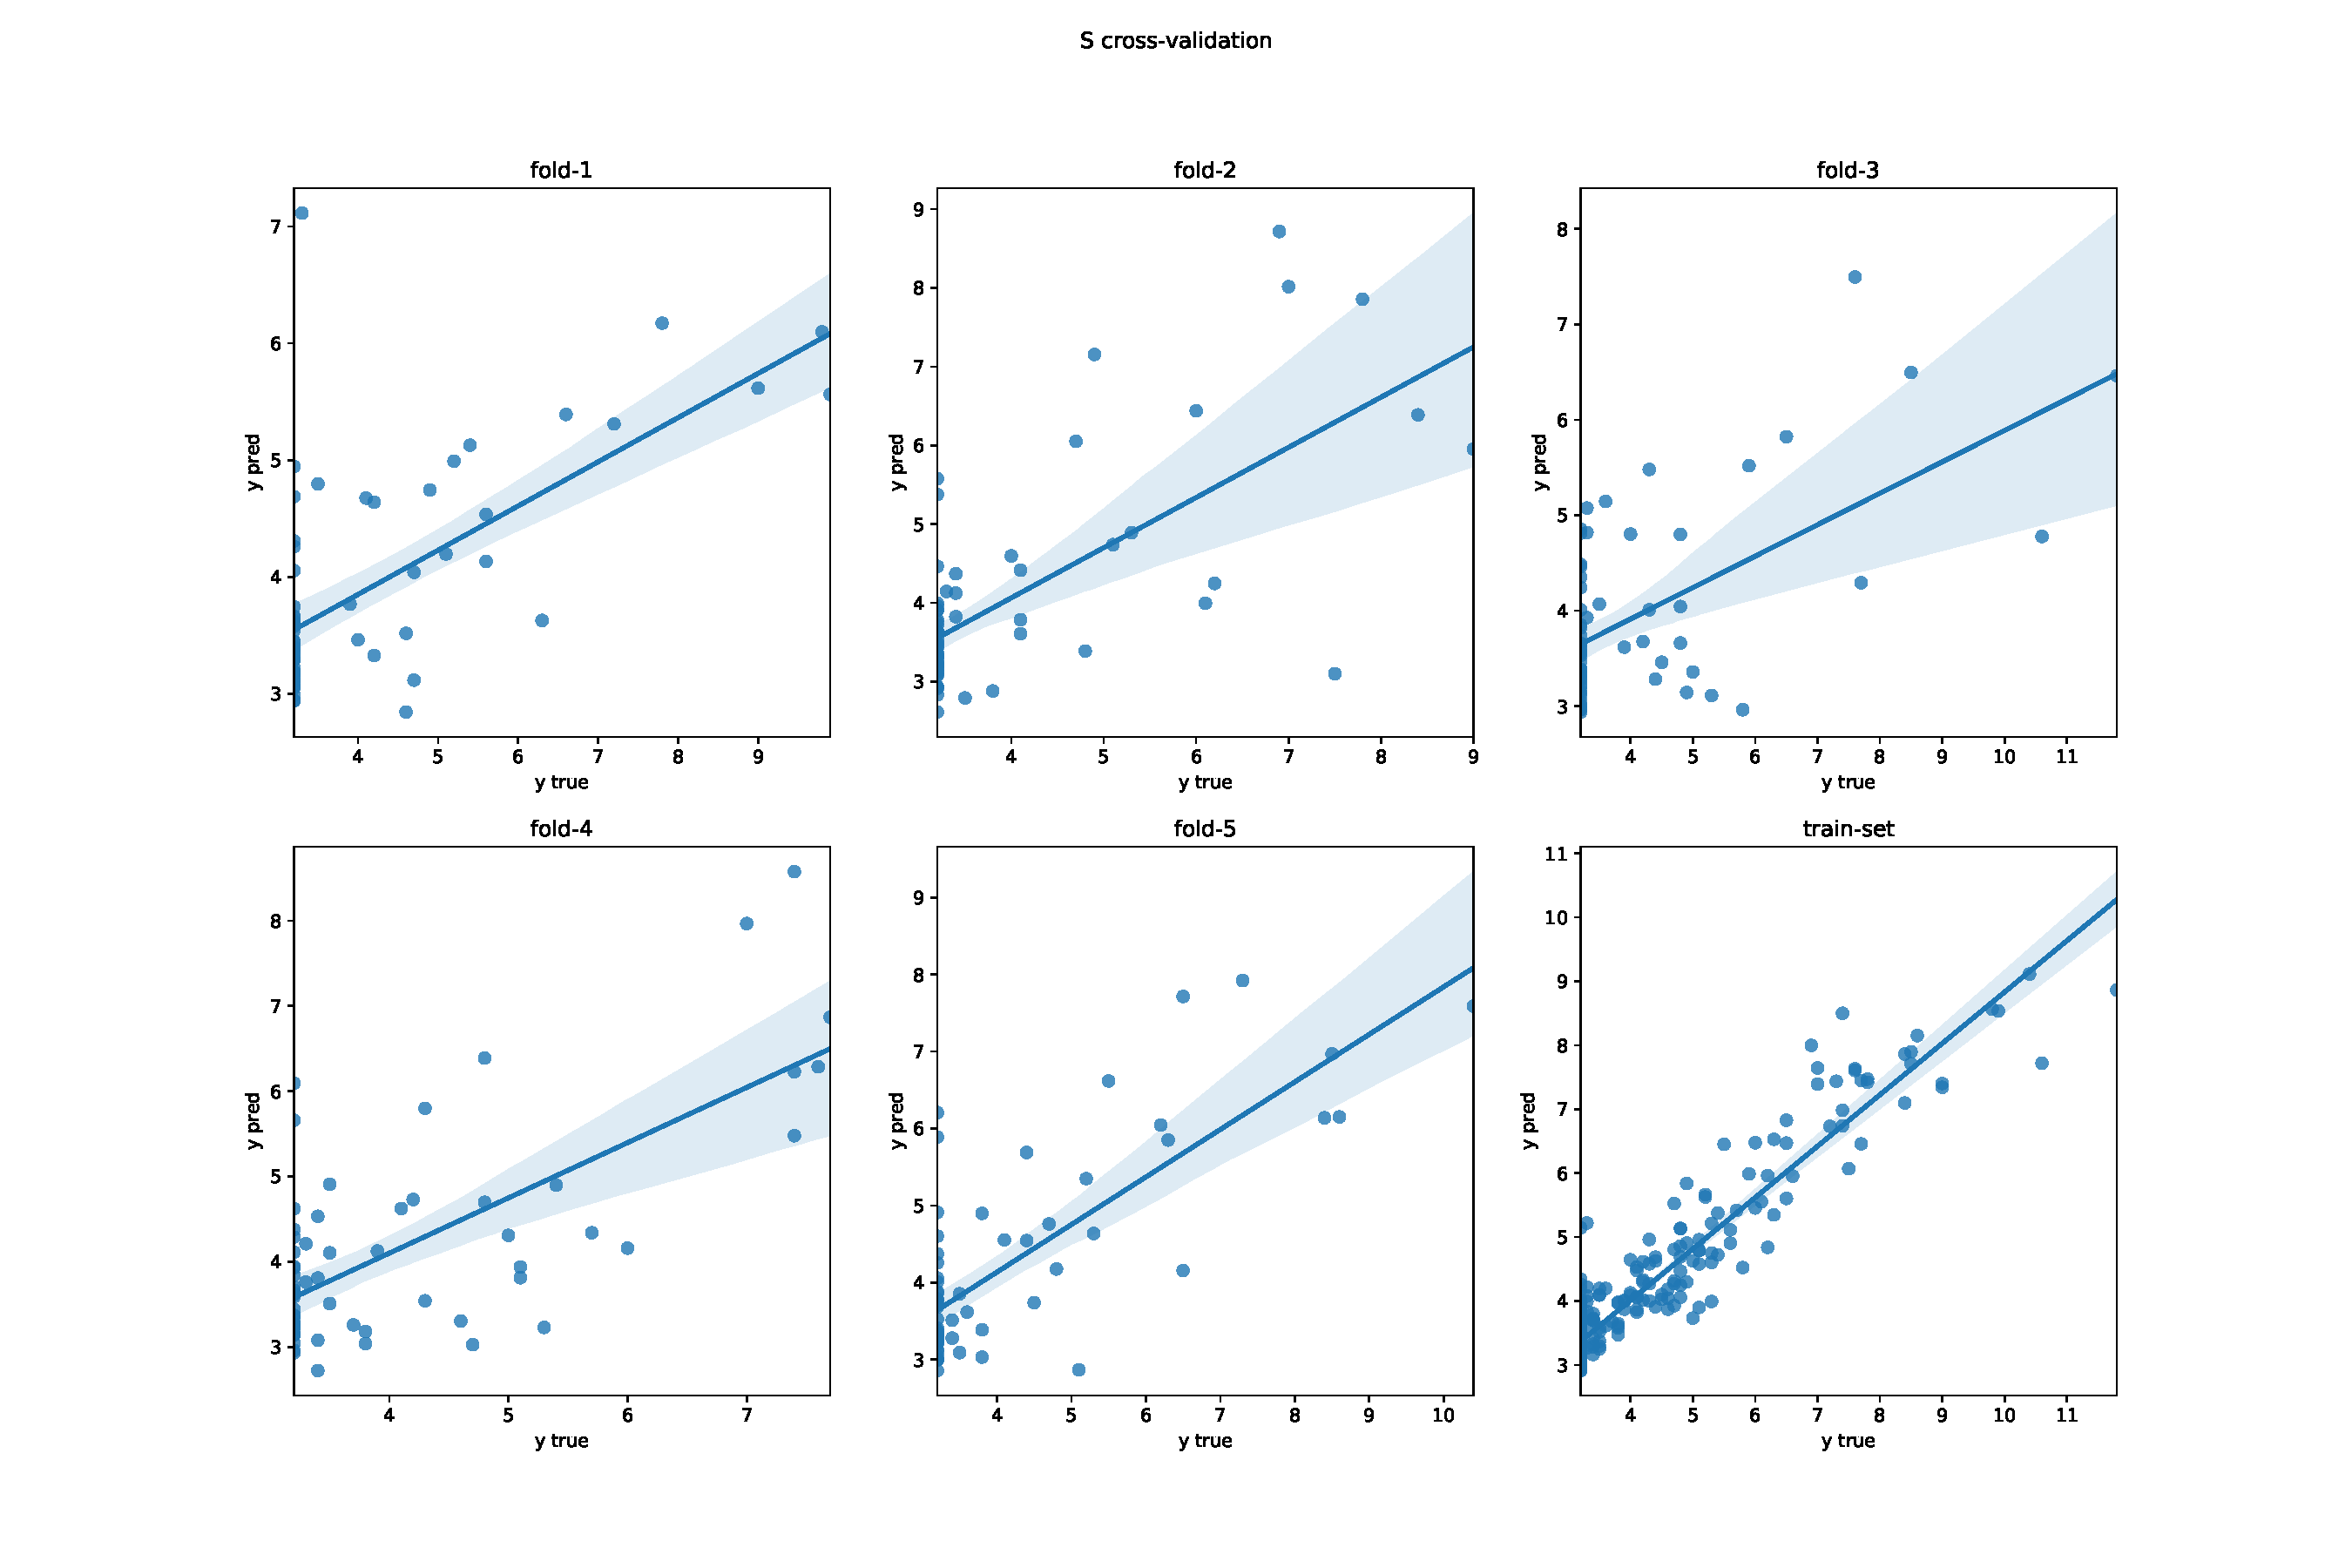
\includegraphics[width=1\textwidth]{S-cross-validation}
%	\caption{对S损失进行交叉验证}
%	\label{RON-loss-cv}
%\end{figure}}

考虑到有硫含量的约束,所以先对操作变量与硫含量的关系进行建模。建模使用的回归器与机器学习管线与章节\ref{sec:modeling}中的相一致,其中特征筛选得到了9个关键变量:'精制汽油出装置硫含量','混氢点氢气流量','还原器温度','D203出口燃料气流量','D-123压力','烟气出对流室温度','冷氮气过滤器ME-114差压','R-102底喷头压差'。其中产品硫含量为常数,其余8个为可调整的操作变量。

分析\textbf{与RON损失相关的11个操作变量}和\textbf{与硫相关的8个操作变量},两者交集为\textbf{“精炼汽油出装置硫含量”}。分析原工业数据的产品硫含量,其中有59个样本的硫含量超过了5$\mu$/g 。故应该先对硫含量进行优化,将325个样本的产品硫含量都优化到5$\mu$/g一下;然后对产品的RON损失值进行优化。因为操作变量“精炼汽油出装置硫含量”与RON损失相关,所以在对RON损失优化的过程中需要增加对产品硫含量的约束,使其满足题设条件;最后,如果有样本优化后仍不满足硫含量的约束,视其为异常样本,将其删除。算法流程图见图\ref{img:opt-flowchat}所示。

\begin{figure}[htb]
	\centering
	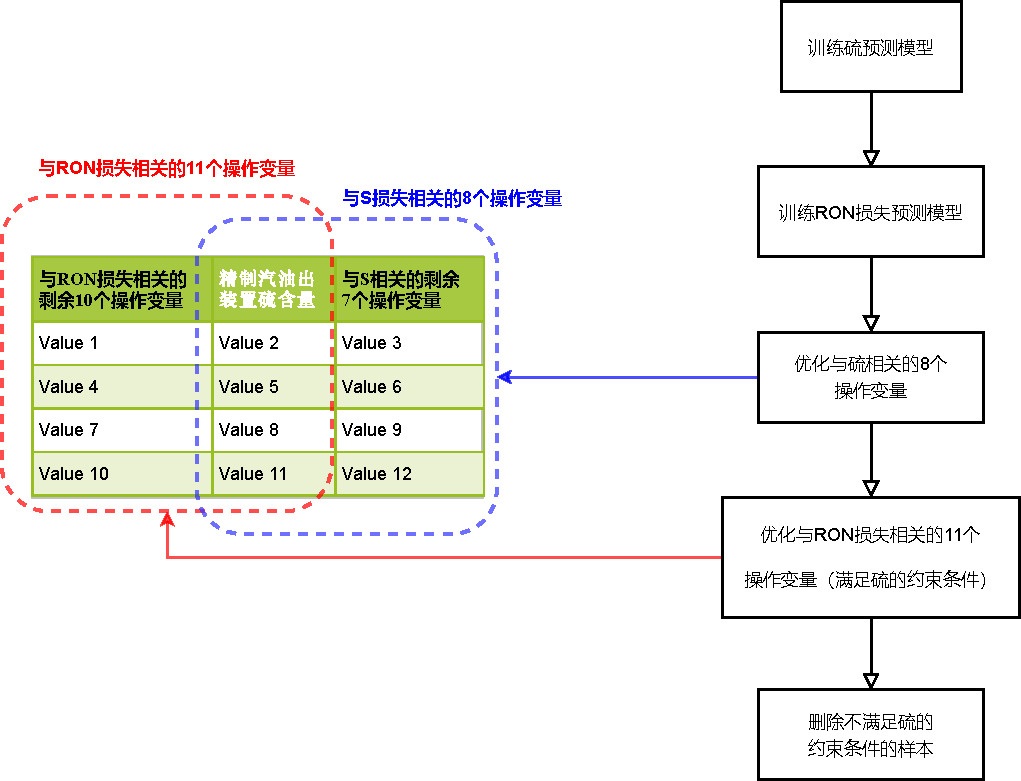
\includegraphics[width=1\textwidth]{opt-flowchat}
	\caption{对RON损失进行交叉验证}
	\label{img:opt-flowchat}
\end{figure}


要求在保证产品硫含量不大于5μg/g的前提下,利用你们的模型获得325个数据样本(见附件四“325个数据样本数据.xlsx”)中,辛烷值(RON)损失降幅大于30%的样本对应的主要变量优化后的操作条件(优化过程中原料、待生吸附剂、再生吸附剂的性质保持不变,以它们在样本中的数据为准)。

<<<<<<< HEAD
要求在保证产品硫含量不大于5μg/g的前提下,利用你们的模型获得325个数据样本(见附件四“325个数据样本数据.xlsx”)中,辛烷值(RON)损失降幅大于30%的样本对应的主要变量优化后的操作条件(优化过程中原料、待生吸附剂、再生吸附剂的性质保持不变,以它们在样本中的数据为准)。
=======
>>>>>>> f155622819f17c9b1ea1bd840c239c0919612e26

\FloatBarrier
\subsubsection{贝叶斯优化与TPE算法简介}

假设有一个函数$f:x\rightarrow \mathbb{R}$ 需要在$x\in X$内找到

\begin{equation}\label{eq:optimation}
	x^*={\arg\min}_{x\in X}f(x)
\end{equation}

当$f$是凸函数且定义域X也是凸的时候,我们可以用已经广泛研究的凸优化来处理,但$f$不一定是凸的。在这种情况下就可以用启发式算法来做全局优化,常见的算法有进化算法、粒子群算法等。但贝叶斯算法具有鲁棒性高、搜索效率高等特点与优点,更适合本题的场景,故在此选择贝叶斯优化来对RON损失和硫含量进行优化。

Sequential model-based optimization (SMBO) 是贝叶斯优化的最简形式,其算法思路如图\ref{img:smbo}所示。

\begin{figure}[htb]
	\centering
	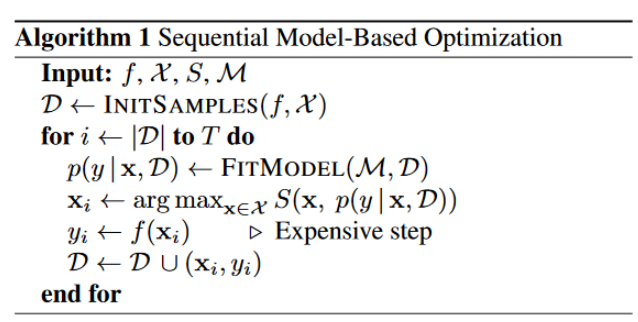
\includegraphics[width=.6\textwidth]{smbo}
	\caption{SMBO算法}
	\label{img:smbo}
\end{figure}

\begin{itemize}
	\item $f$:评价函数,在本题中是章节\ref{sec:modeling}得到的预测模型
	\item $X$:搜索空间,在本题中是与RON损失或硫相关的主要操作变量。
	\item $D$:表示数据组成的数据集,在本题中是原工业数据。
	\item $S$:是\textbf{Acquisition Function}(采集函数),用来评价采样样本的好坏,一般采用EI函数,见公式\eqref{eq:EI}。
	\item $\mathit{M}$:是对数据集D进行拟合得到的模型,如随机森林、高斯过程等。本题使用TPE模型。
\end{itemize}

\begin{equation}\label{eq:EI}
	EI(X)=\mathbb{E}_{max}(f(x)-f(x^+), 0)
\end{equation}

TPE全称Tree-structured Parzen Estimator,是用GMM(Gaussian Mixture Model)来学习超参模型的一种方法。

首先根据 Bayes 定义,$p(x|y)$ 即模型 $loss$ 为 $y$ 的时候超参为 $x$ 的条件概率。第一步,我们根据已有的数据选取一个 $loss$ 的阈值 $y^*$,一般为15\%的分位数。对大于阈值和小于阈值的数据,分别学习两个概率密度 $l(x)$ 和 $g(x)$ 。

\begin{equation}\label{eq:lxgx}
	p(x|y)=\left\{
	\begin{aligned}
		l(x) &  & if \ y<y^* \\
		g(x) &  & if \ y\ge y^* \\
	\end{aligned}
	\right.
\end{equation}

根据EI公式\eqref{eq:EI},将其带入公式\eqref{eq:lxgx},发现只要能${\arg\min}_x{g(x)/l(x)}$就能${\arg\min}_x{EI(x)}$。

\begin{equation}\label{EIlxgx}
	EI_{y^*}(x) \propto (\gamma+\frac{g(x)}{l(x)}(1 - \gamma))^{-1}
\end{equation}

综上,TPE的原理就是建立两个分布:优势样本的分布于劣势样本的分布。TPE在每次迭代中按照这样的规则去采样:采样的样本在优势样本分布$l(x)$中的概率密度尽量大,在劣势样本分布$g(x)$中的概率密度尽量小,本质上是逐渐增大在优势样本附近采样率的一个启发式优化过程。




\FloatBarrier
\subsubsection{对产品硫含量进行优化}


原工业数据的产品硫含量的分布图见图\ref{img:origin-S-dist},其中大于5$\mu g/g$的样本有59个,占 $18.15\%$。

可以看到原工业数据的产品硫含量为长尾分布,充斥着大量硫含量偏高的样本。


\begin{figure}[htb]
	\centering
	\begin{minipage}[c]{0.4\textwidth}
		\centering
		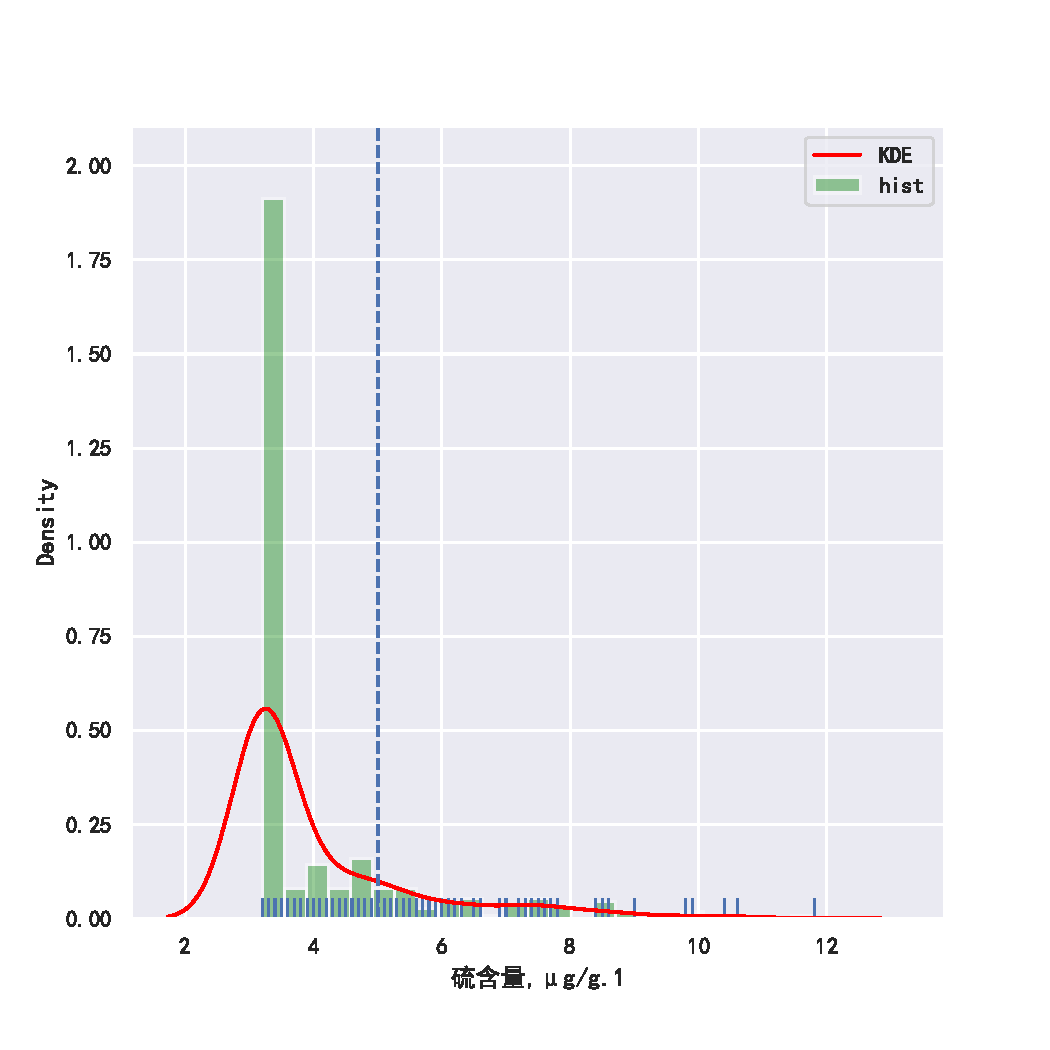
\includegraphics[height=0.3\textheight]{S-dist}
		\subcaption{原工业数据硫含量的分布图}
		\label{img:origin-S-dist}
	\end{minipage}
	\begin{minipage}[c]{0.4\textwidth}
		\centering
		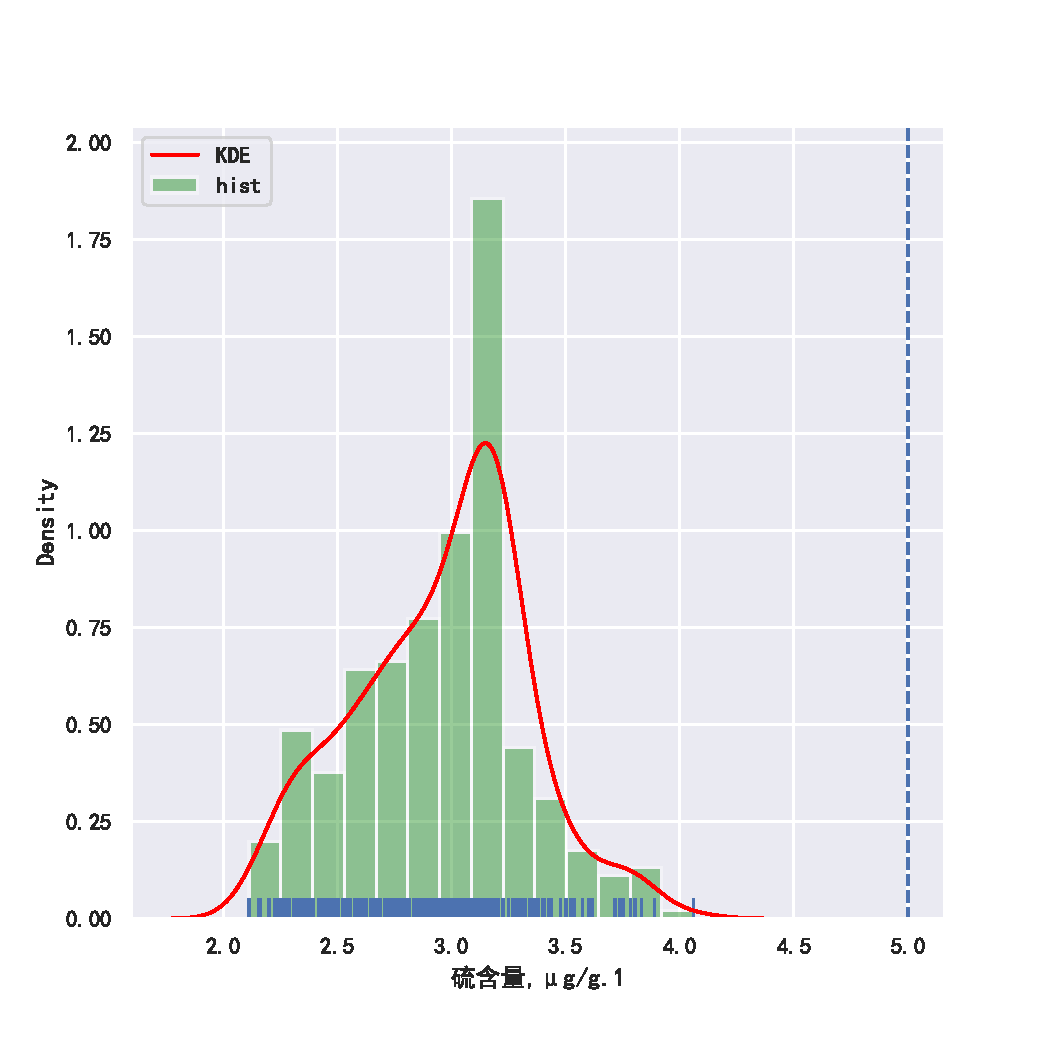
\includegraphics[height=0.3\textheight]{S-dist(after-opt)}
		\subcaption{单独对与硫优化后的分布图}
		\label{img:single-S-dist}
	\end{minipage}
	\begin{minipage}[c]{0.4\textwidth}
		\centering
		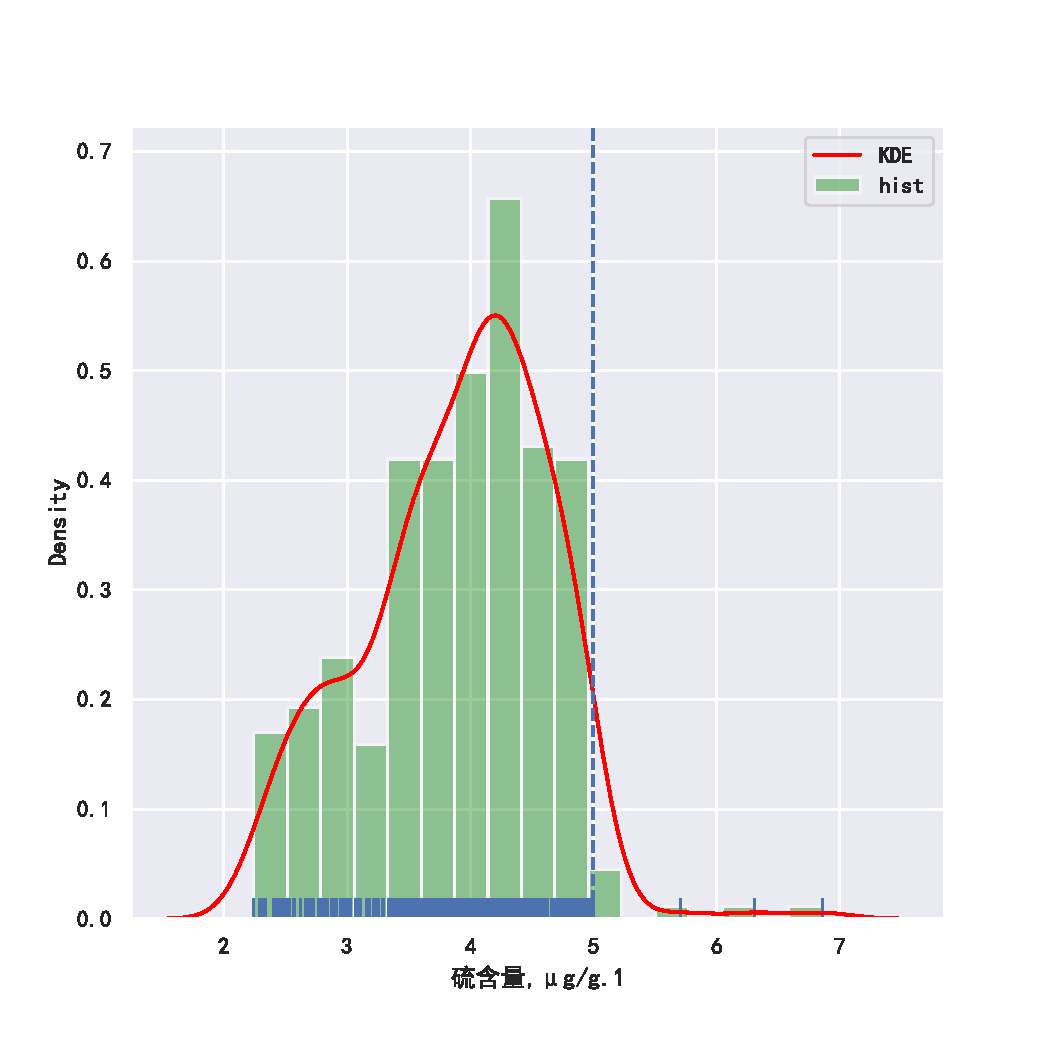
\includegraphics[height=0.3\textheight]{S-dist(after-RON-opt)}
		\subcaption{对RON损失优化后硫的分布图}
		\label{img:joint-S-dist}
	\end{minipage}
	\caption{313号样本处理2中的3个变量}
\end{figure}



以与硫含量相关的8个主要变量(见章节\ref{sec:opt-problem-analyze})作为待优化变量,并根据操作变量的取值范围得到一个参数空间$\mathbb{H}_S \in \mathbb{R}^8$。
用之前得到的硫预测模型作为优化过程的评价函数$g(s), s\in \mathbb{H}_S$,
用贝叶斯优化库\texttt{HyperOpt}的TPE算法对工业数据的325个样本逐一进行优化,每次优化迭代50次。

单独对参数空间$\mathbb{H}_S$优化后,产品硫含量的分布图见图\ref{img:single-S-dist}。可以看到产品的硫分布被压缩到了区间$[0,5)$中了。



\FloatBarrier
\subsubsection{对RON损失进行优化}

以与RON损失含量相关的11个主要变量(见表\ref{tab:003})作为待优化变量,并根据操作变量的取值范围得到一个参数空间$\mathbb{H}_R \in \mathbb{R}^{11}$。
用之前得到的RON损失预测模型作为评价函数$f(r), r\in \mathbb{H}_R$。



但实际使用时并不能直接用$f(r)$作为优化过程的评价函数。如流程图\ref{img:opt-flowchat}所示,硫与RON损失有一个操作变量重合,虽然在上一步中通过调整与硫相关的8个操作变量是的目前产品硫含量大幅下降,但是在优化RON损失的过程中可能在调整这一重合的操作变量时会导致产品硫含量超出题设范围。故对RON损失的评价函数做出调整,如公式\eqref{eq:RON-evaluation}所示,用调整后的$\hat{f}(r)$代替$f(r)$:

\begin{equation}\label{eq:RON-evaluation}
	\hat{f} = f(r)+{\infty \times \max({0},{g(s)-5}) } \ \ \ \ r\in \mathbb{H}_R \ \ s\in \mathbb{H}_S 
\end{equation}

\begin{figure}[htb]
	\centering
	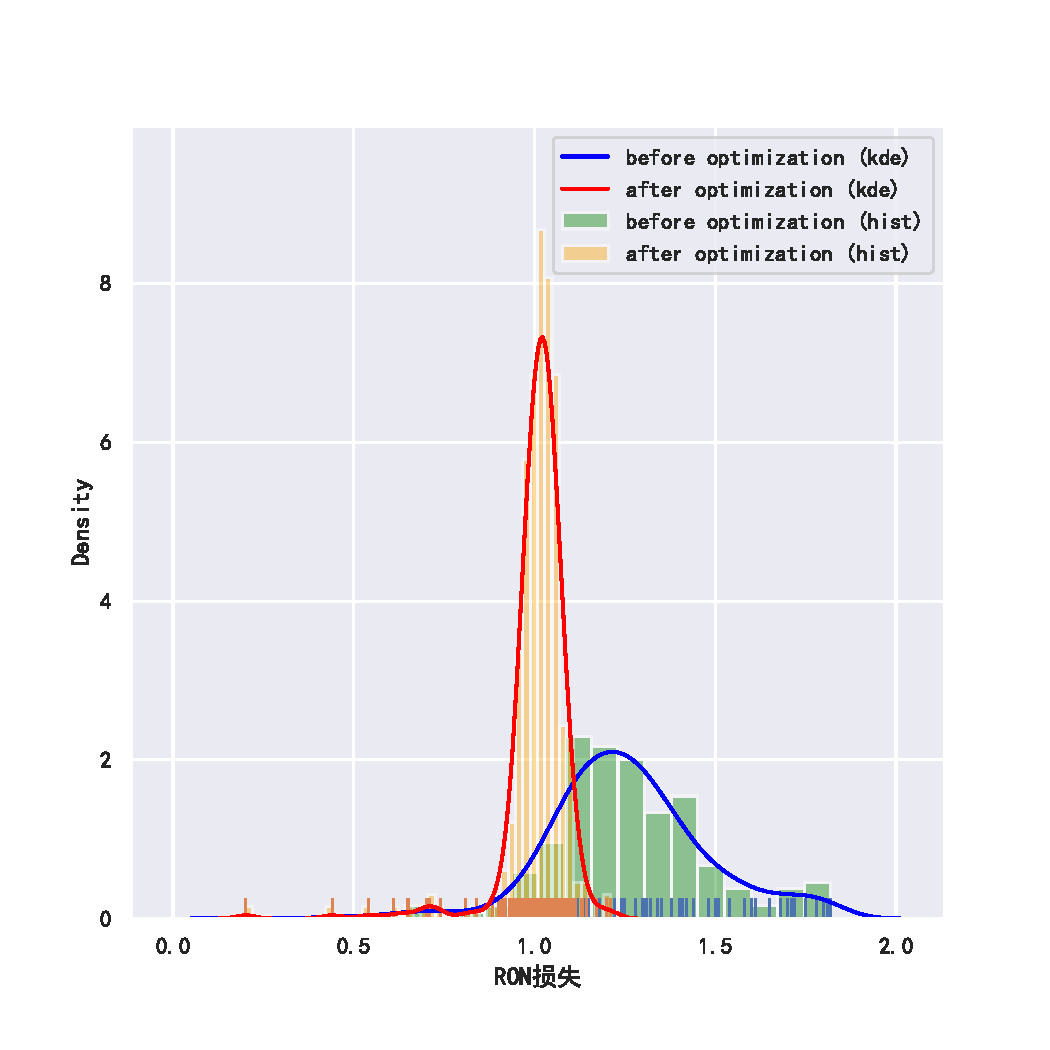
\includegraphics[width=.5\textwidth]{RON-dist}
	\caption{优化前后的RON损失分布图}
	\label{img:RON-compare}
\end{figure}

更新评价函数后,如之前的操作,对工业数据的325个样本逐一进行优化,每次优化迭代50次。优化前后RON损失的分布图如图\ref{img:RON-compare}所示,可见RON损失在优化后被压缩到了$[0.8, 1.2]$附近的区域。

优化后产品硫含量分布如图\ref{img:joint-S-dist}所示,可见分布在$S=5$处呈截断的痕迹,但仍有3个样本超出了$S\le 5$的限制,这3个样本在表\ref{tab:exceed-S-constraint}中列出。

\begin{table}[htb]
	\caption{3个优化后不符合约束条件的异常样本}\label{tab:exceed-S-constraint} \centering
	\begin{tabular}{ccccc}
		\toprule[1.5pt]
		time &  原硫含量($\mu g/g$) &  优化后硫含($\mu g/g$) &  原RON损失 &  优化后RON损失 \\
		\midrule[1pt]
		2017/11/10 8:00:00 &              4.2 &               6.30 &    1.10 &      0.99 \\
		2017/11/6 8:00:00 &              6.2 &               5.70 &    1.10 &      0.91 \\
		2017/9/18 8:00:00 &              3.8 &               6.86 &    1.21 &      0.89 \\  
		\bottomrule[1.5pt]
	\end{tabular}
\end{table}

优化后,有55个样本的RON损失降幅大于30\%,占比为16.92\%。RON损失降幅情况见图\ref{img:RON-loss-descrease}。

\begin{figure}[htb]
	\centering
	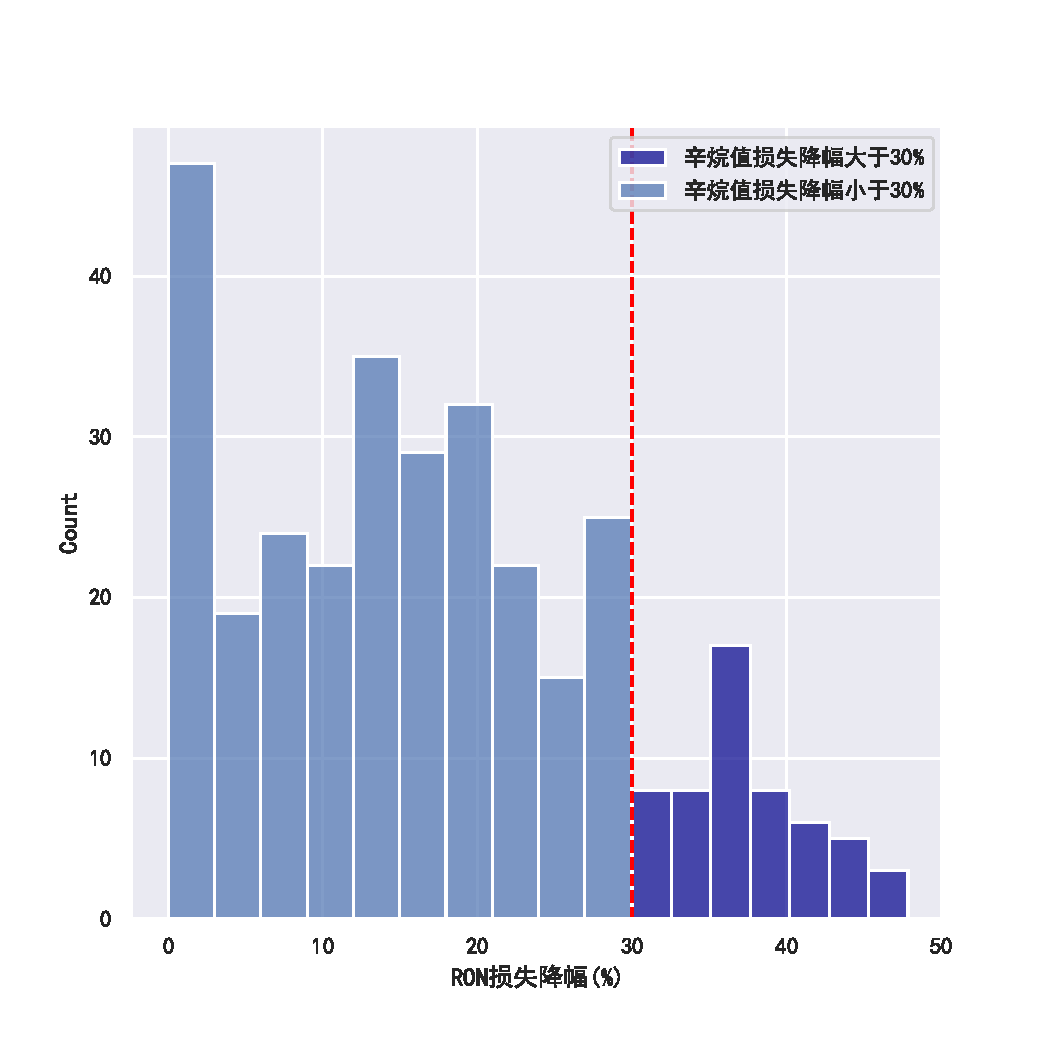
\includegraphics[width=.5\textwidth]{RON-loss-decrease}
	\caption{RON损失降幅直方图}
	\label{img:RON-loss-descrease}
\end{figure}


为了更好地对比优化RON损失前后主要操作变量的变化情况,绘制了11个主要操作变量和产品辛烷值(常量)的分布图,如图\ref{img:main-op-opt-0}和图\ref{img:main-op-opt-1}所示。

\begin{figure}[htb]
	\centering
	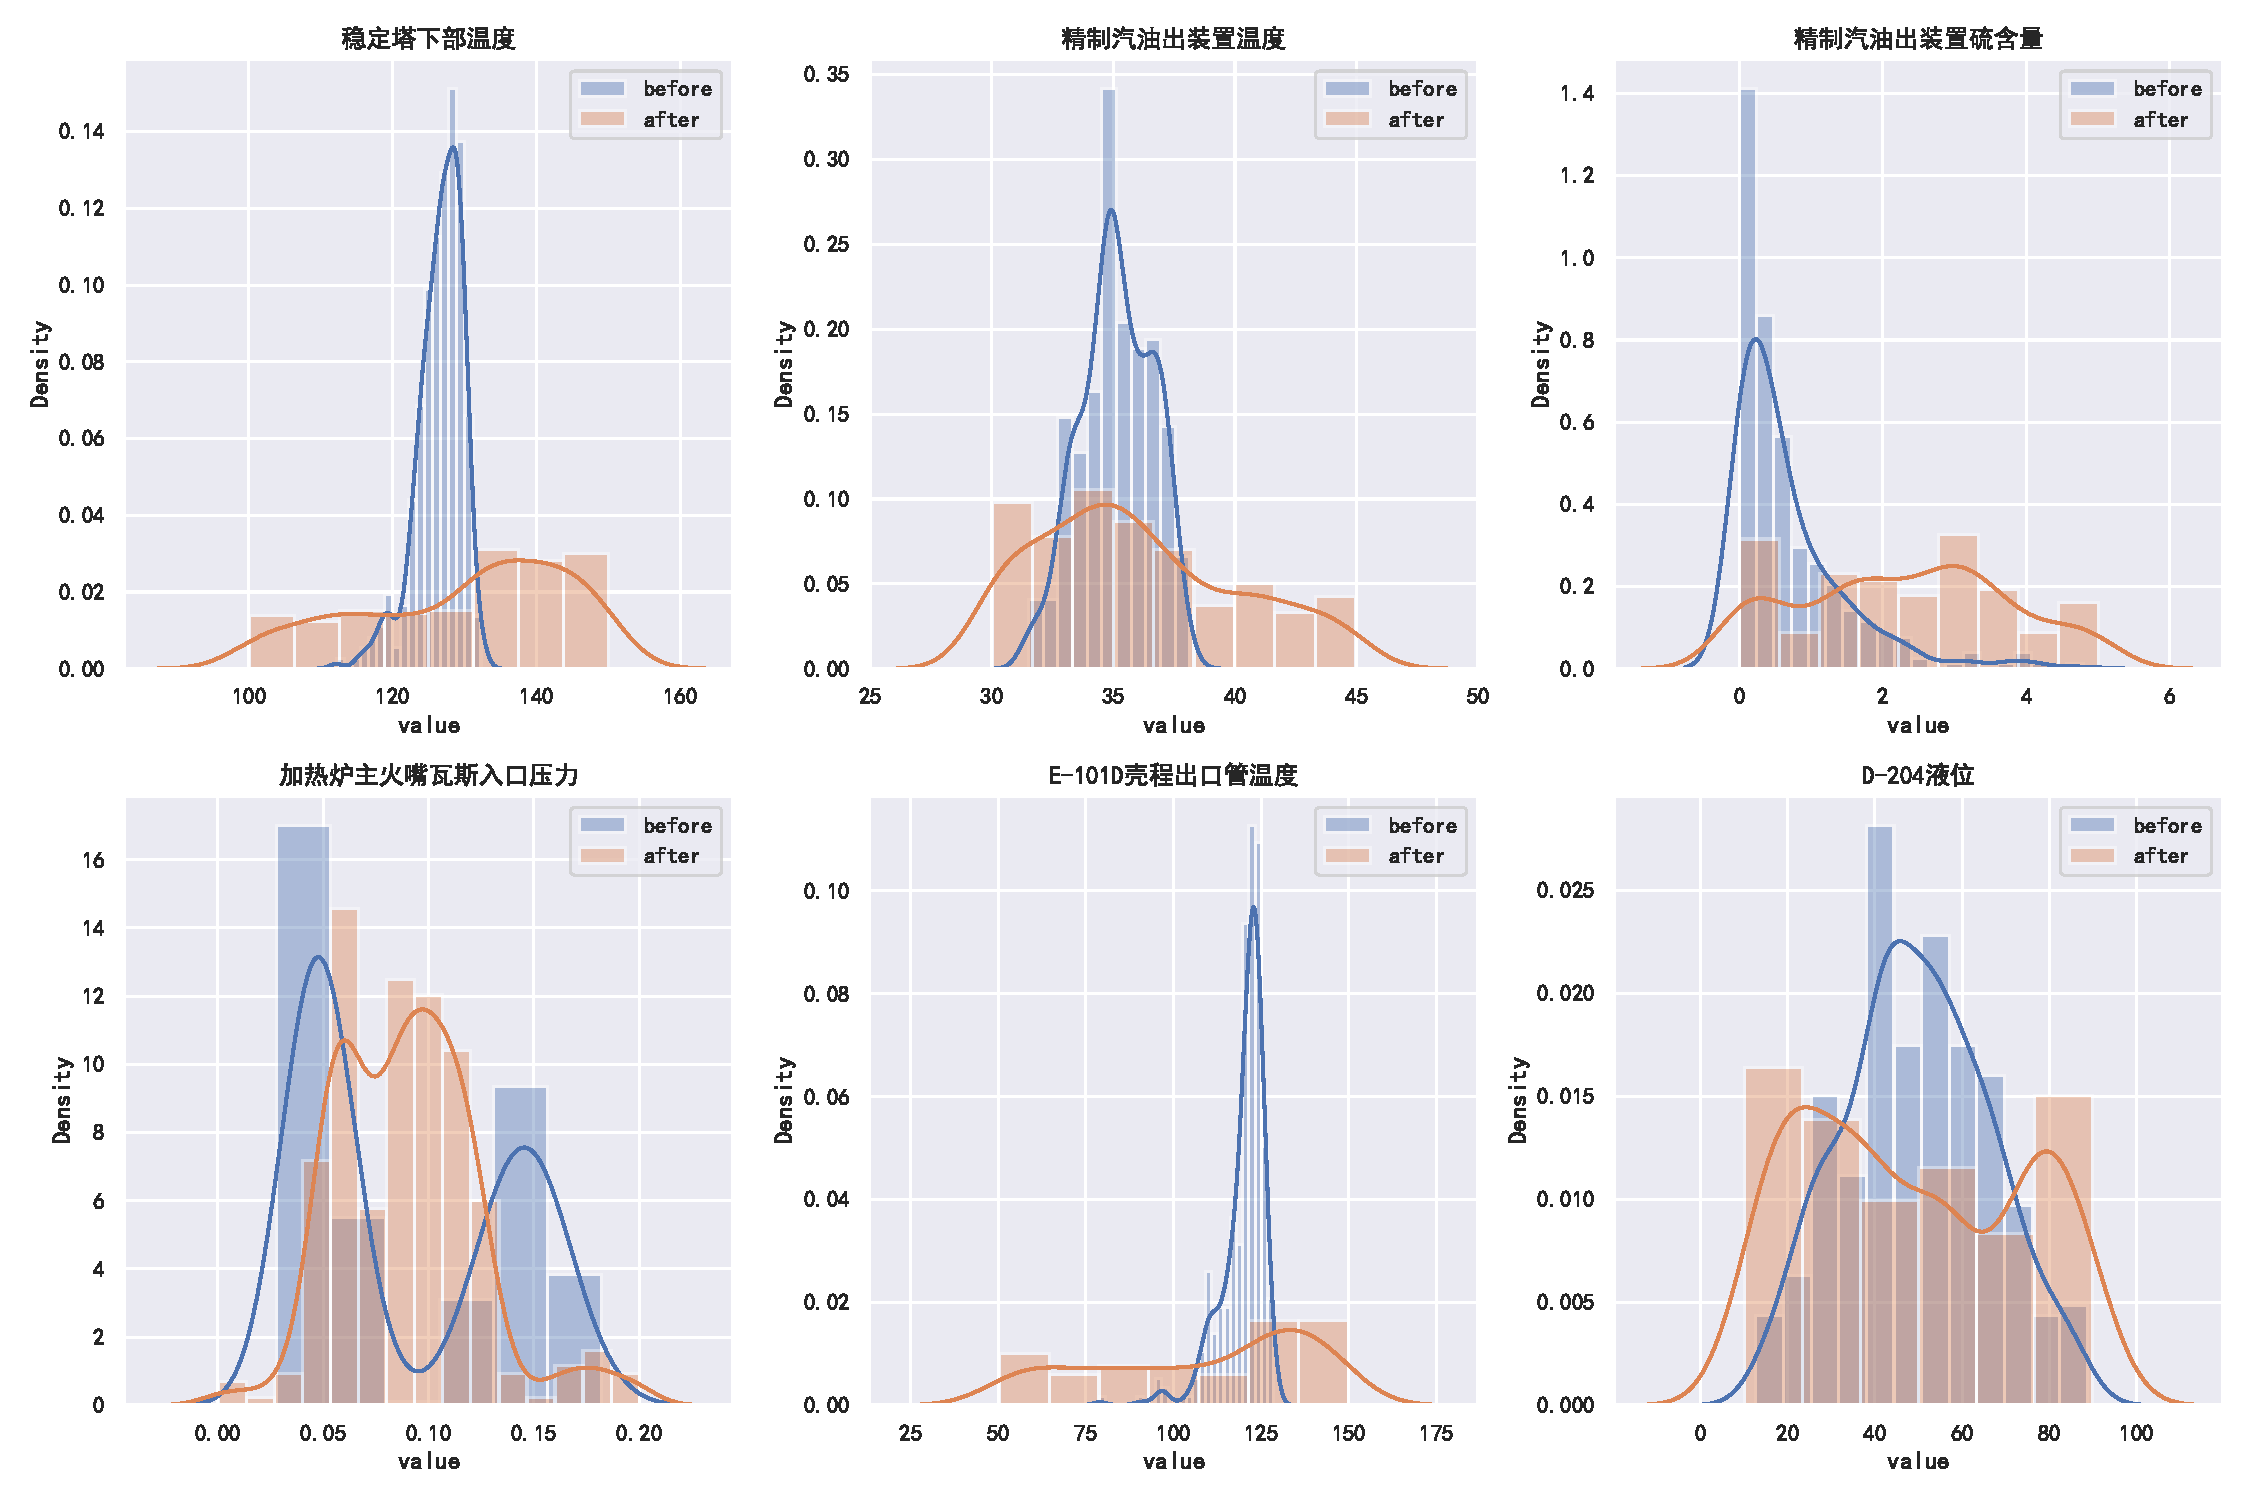
\includegraphics[width=0.85\textwidth]{main-op-opt-0}
	\caption{优化前后6个操作变量的分布}
	\label{img:main-op-opt-0}
\end{figure}

\begin{figure}[htb]
	\centering
	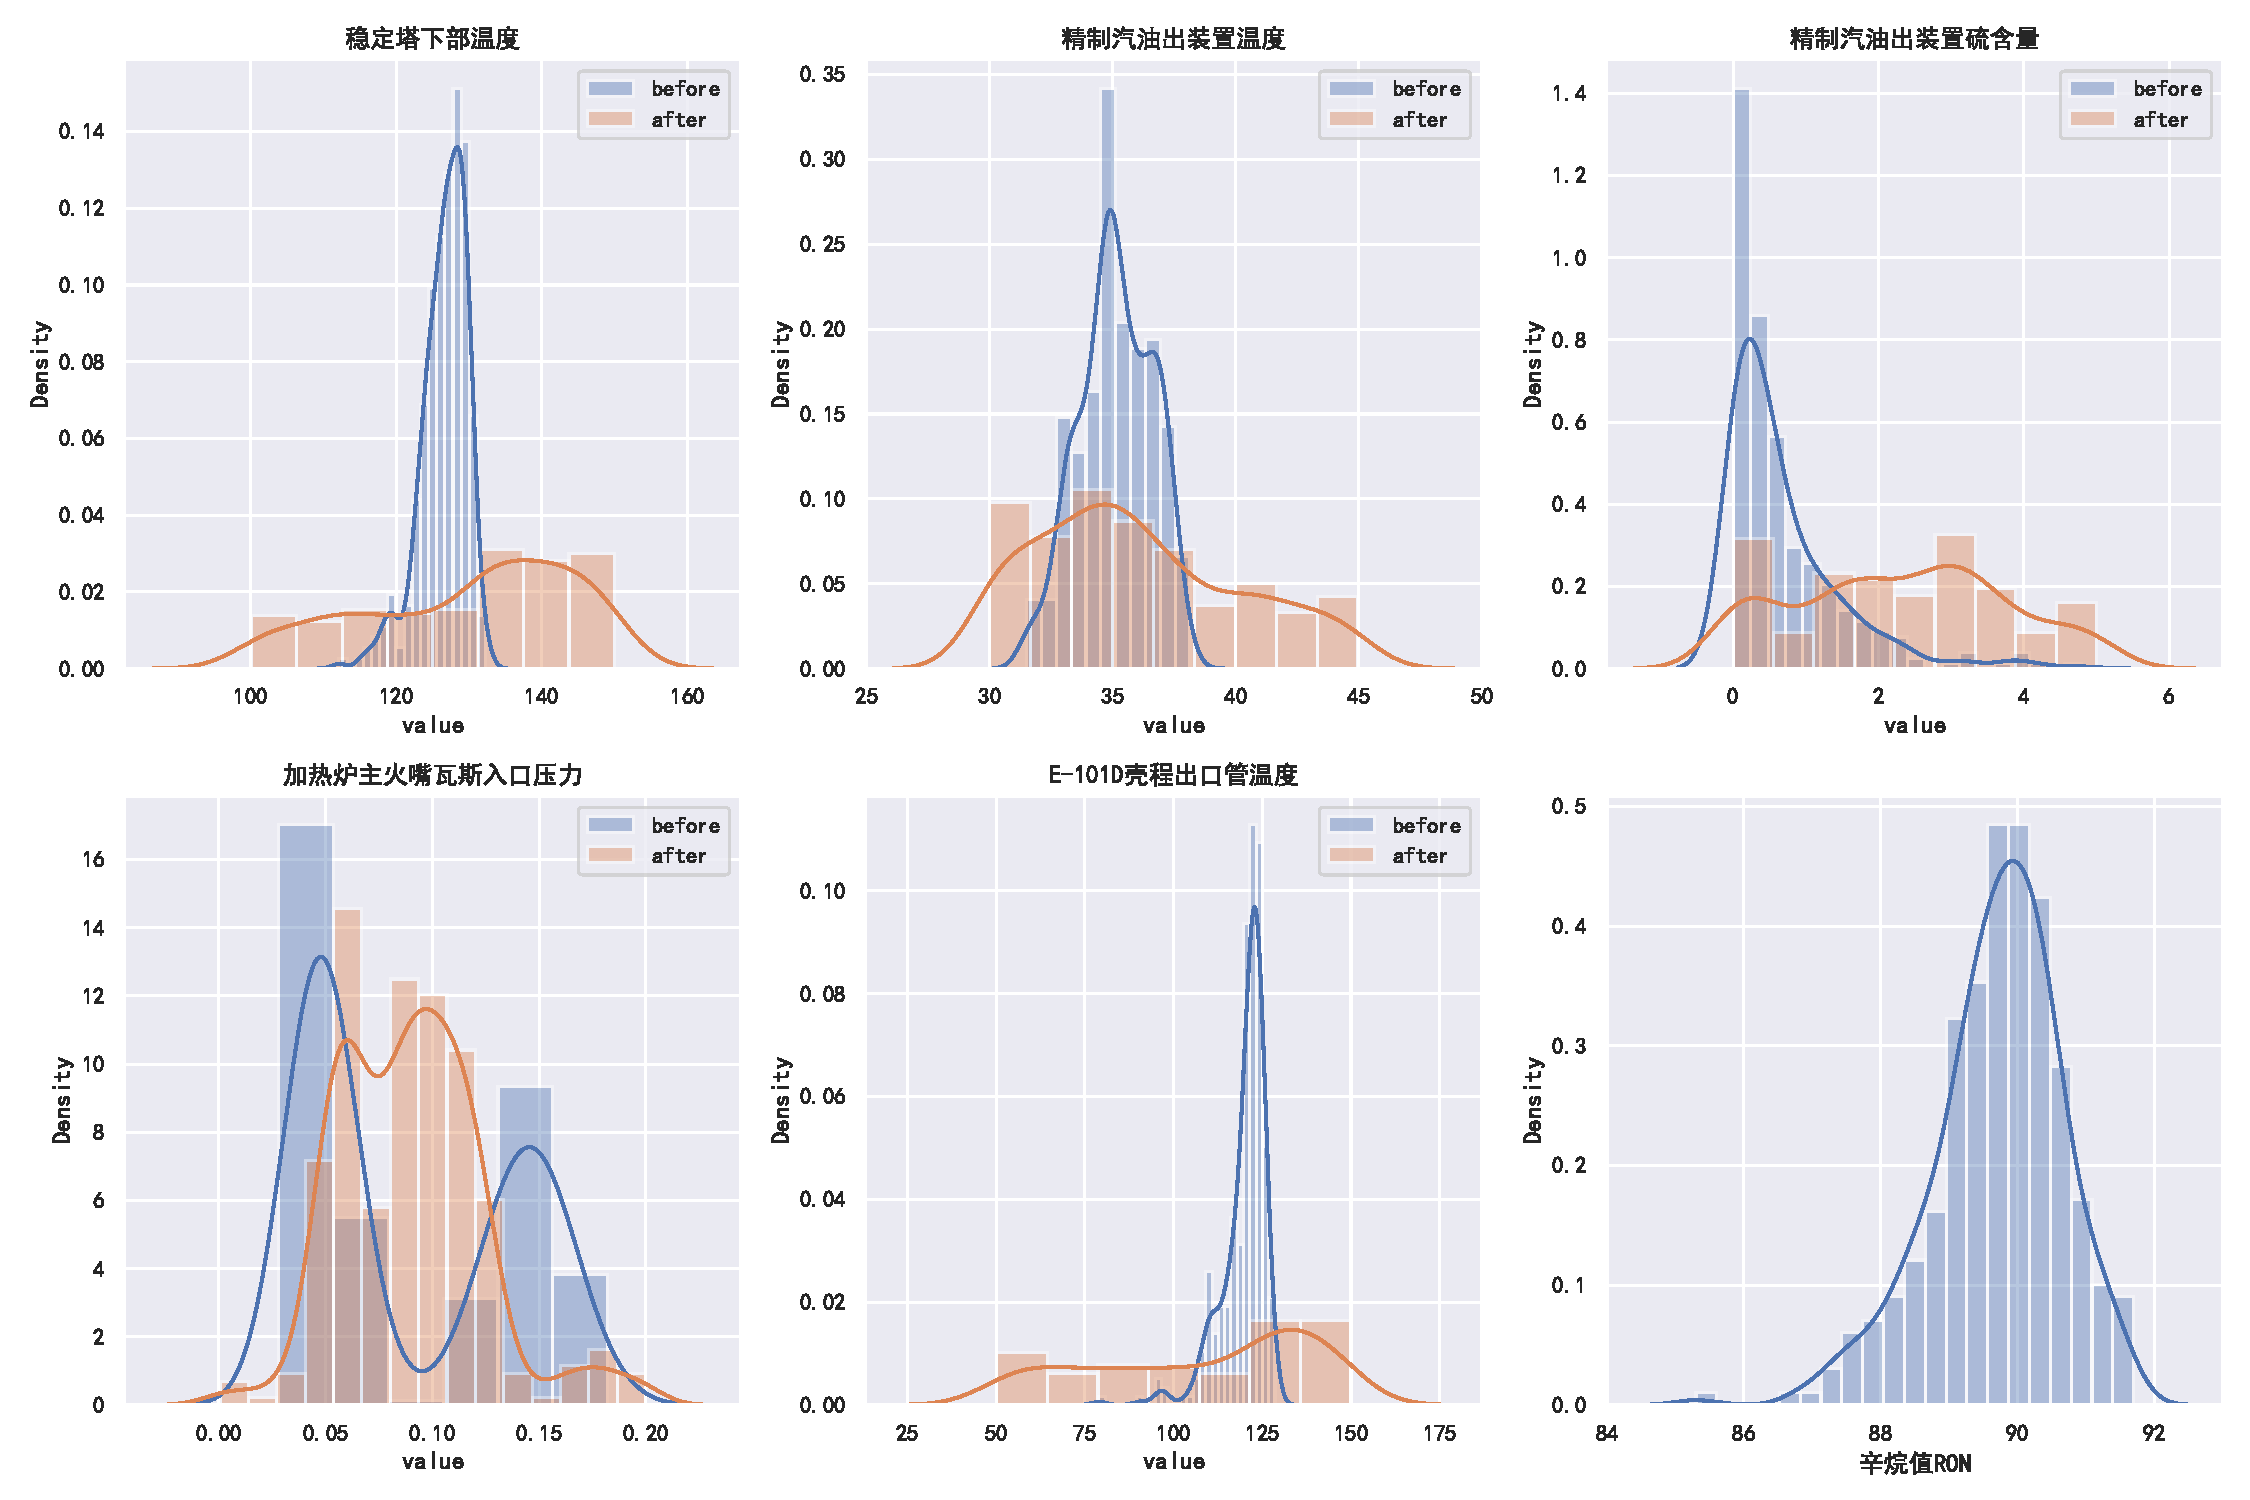
\includegraphics[width=0.85\textwidth]{main-op-opt-1}
	\caption{RON与优化前后的5个操作变量的分布}
	\label{img:main-op-opt-1}
\end{figure}

\FloatBarrier
\subsection{问题五:模型的可视化展示}

\FloatBarrier
\subsubsection{问题分析}

本文已经在问题三的解答中选出了12个主要变量,在问题四中对包括133样本在内的许多样本进行了优化,其中133样本可以通过改变一些操作变量实现在硫含量不高于5(5μg/g)的情况下辛烷值损失降低至0.8828。而在这一问我们需要找出由原先的操作条件,逐步调整为优化后的操作条件的调整路径,使得每一次调整幅度不超过操作变量每次允许调整幅度值Δ,同时,每一步操作变量对应的状态产生的硫不应该高于5μg/g。而且,操作变量调整过程中不应超出变量的操作范围(操作变量的范围由经验值以及附件中给出的操作变量信息共同划定)。

\FloatBarrier
\subsubsection{问题建模}
考虑到工程实际情况,在此使用改进的启发式搜素A*算法求解该问题。本问题的处理流程图及A*算法的流程图如下:
\begin{figure}[H]
	\centering
	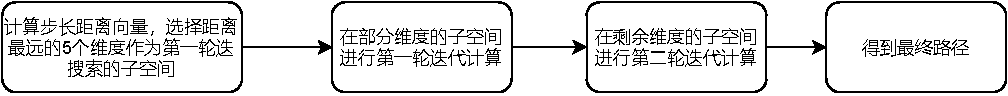
\includegraphics[width=1.0\textwidth]{5lct}
	\caption{模型的可视化展示总体流程图}
\end{figure}

\begin{figure}[H]
	\centering
	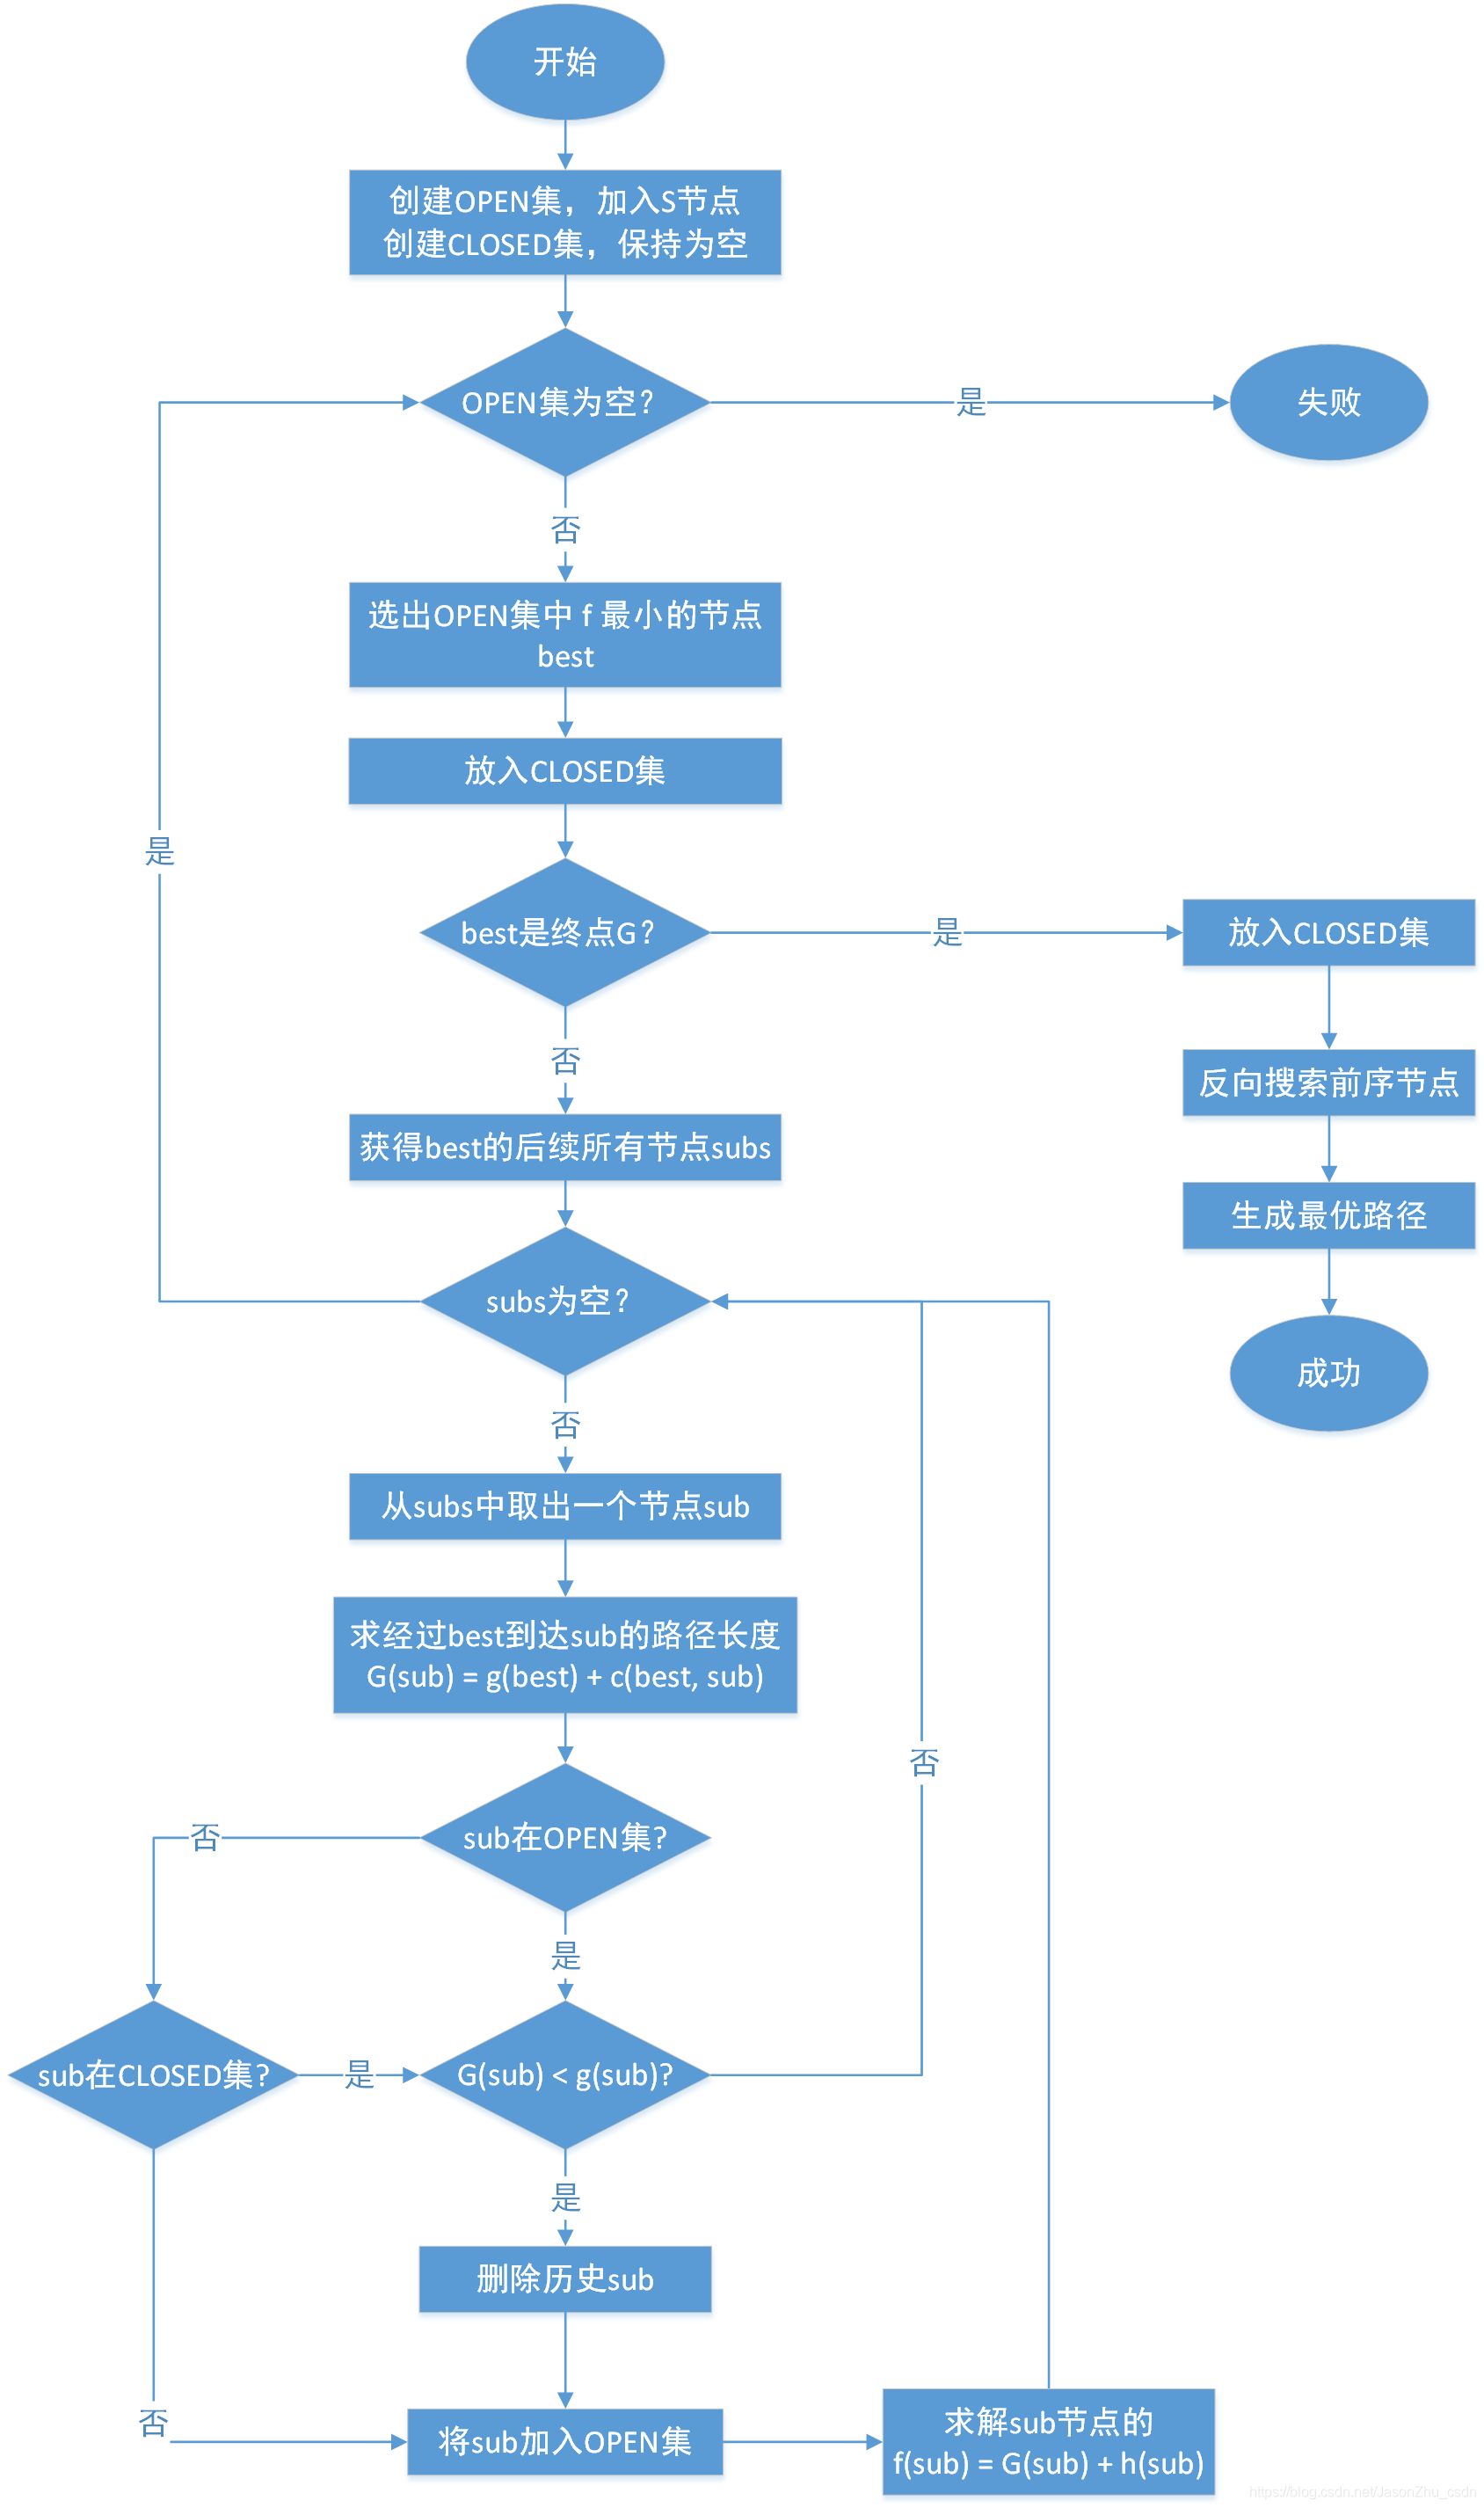
\includegraphics[width=0.8\textwidth]{axing}
	\caption{A*算法的流程图}
\end{figure}
对该问题建模如下:首先12个主要变量中,只有11个是操作变量,这11维操作变量的数值可以看成11维空间中的一个位置的坐标。记原始的坐标为x,第四问优化后的变量为y,所以实际就是求解在11维空间中由x到y的一条路径,其中路径的途径点不能超过所有变量的取值范围组成的11维立方体,且不能经过11维立方体中使硫产量大于5的区域,路径应尽量短,而且每一步在每一个维度上步幅都不应超过对应操作变量允许调整的幅度值Δ。为简化问题以及减少计算量,假设每一个操作变量的每一次调整都刚好等于Δ(最后一步除外,最后一次是小于等于Δ)。第三问得到的预测硫和辛烷值损失的模型记为硫产量$S=S(x)$,辛烷值损失$RON\_LOSS=N(x)$。


\FloatBarrier
\subsubsection{模型优化}

在建模过程中发现,在11维空间中运行A*算法需要非常巨大的计算资源,于是进一步优化计算模型,得到的计算公式如下:
\begin{align}
\vec{d }&=\left | \left ( \vec{y}-\vec{x} \right ) \right |\\
\overrightarrow{step }&= \vec{d }./{\overrightarrow{\Delta} }
\end{align}
式(15)中./代表向量运算中的点除。用起始点x与终点y坐标的距离向量,元素除以对应的Δ,然后向上取整,得到一个11维向量,每个维度的值代表每个维度上起始点x与终点y的步长距离,经过计算得到11维向量\:$[4, 1, 6, 2, 3, 2, 59, 4, 3, 3, 6]$,
经过观察发现只有少数维度步长距离较远,大部分维度距离并不远,于是我们决定将A*算法修改为两轮计算,每一轮都只在部分维度组成的子空间中找通往目的地的通路(其他维度保持不变),只要每一轮都可以找到这样符合上文所述约束条件的通路,那么两个通路链接起来,就是完整的从起点到终点的一条道路。
从中选取步长距离较远的$index=[0,2,6,7,10]$维度进行第一轮优化,其他维度保持不变,当挑选的这些维度都优化到y点对应维度的值时,第一轮优化结束,此时的坐标为
x1=[121.3461, 34.4524, 4.9924, 0.0386, 120.7679, 52.7805, 321.5952, 32.7367, 8.8462,410.3512,-2.2292]对应的RON\_损失,  S为1.0422, 4.3748。接着,保持$index=[0,2,6,7,10]$对应的坐标值不变,对剩余的6个维度进行第二轮优化,优化结束后最终坐标等于[121.3461,34.2690,4.9924,0.1060,123.3863,59.77
<<<<<<< HEAD

=======
=======
>>>>>>> f155622819f17c9b1ea1bd840c239c0919612e26
建模过程中发现,在11维空间中运行A*算法需要非常巨大的计算资源,于是必须决定进一步优化计算模型,计算公式如下:
\begin{equation}
	\overrightarrow{d}= \left | \left ( \overrightarrow{y}-\overrightarrow{x}\right ) \right |
\end{equation}
\begin{align}
	\overrightarrow{step} & = \frac{\vec{d }}{\overrightarrow{\Delta} }  
\end{align}

用起始点x与终点y坐标的距离向量,元素除以对应的Δ,然后向上取整,得到一个11维向量,每个维度的值代表每个维度上起始点x与终点y的步长距离,得到11维向量\:$[4, 1, 6, 2, 3, 2, 59, 4, 3, 3, 6]$,
发现只有少数维度步长距离较远,大部分维度距离并不远,于是我们决定将A*算法修改为两轮计算,每一轮都只在部分维度组成的子空间中找通往目的地的通路(其他维度保持不变),只要每一轮都可以找到这样符合上文所述约束条件的通路,那么两个通路链接起来,就是完整的从起点到终点的一条道路。
从中选取步长距离较远的$index=[0,2,6,7,10]$维度进行第一轮优化,其他维度保持不变,当我们挑选的这些维度都优化到y点对应维度的值时,第一轮优化结束,此时的坐标为
<<<<<<< HEAD
x1=[121.3461, 34.4524, 4.9924, 0.0386, 120.7679, 52.7805, 321.5952, 32.7367, 8.8462,410.3512,-2.2292]对应的RON\_LOSS,  S为1.0422, 4.3748。接着,保持$index=[0,2,6,7,10]$对应的坐标值不变,对剩余的6个维度进行第二轮优化,优化结束后最终坐标等于[121.3461,34.2690,4.9924,0.1060,123.3863,59.7742,321.5952,32.7367,11.2289,412.8519,-2.2292],即为第四问中求出的优化后操作变量值。
x1=[121.3461, 34.4524, 4.9924, 0.0386, 120.7679, 52.7805, 321.5952, 32.7367, 8.8462,410.3512,-2.2292]对应的RON\_LOSS,  S为1.042
2, 4.3748。接着,保持$index=[0,2,6,7,10]$对应的坐标值不变,对剩余的6个维度进行第二轮优化,优化结束后最终坐标等于[121.3461,34.2690,4.9924,0.1060,123.3863,59.7742,321.59
52,32.7367,11.2289,412.8519,-2.2292],即为第四问中求出的优化后操作变量值。
=======
x1=[121.3461, 34.4524, 4.9924, 0.0386, 120.7679, 52.7805, 321.5952, 32.7367, 8.8462,410.3512,-2.2292]对应的RON\_LOSS,  S为1.0422, 4.3748。接着,保持$index=[0,2,6,7,10]$对应的坐标值不变,对剩余的6个维度进行第二轮优化,优化结束后最终坐标等于[121.3461,34.2690,4.9924,0.1060,123.3863,59.77
>>>>>>> Stashed changes
42,321.5952,32.7367,11.2289,412.8519,-2.2292],即为第四问中求出的优化后操作变量值。
>>>>>>> f155622819f17c9b1ea1bd840c239c0919612e26
将每一轮迭代中的硫产量,辛烷值损失,及相关操作变量画成曲线如图所示:
\begin{figure}[htb]
	\centering
	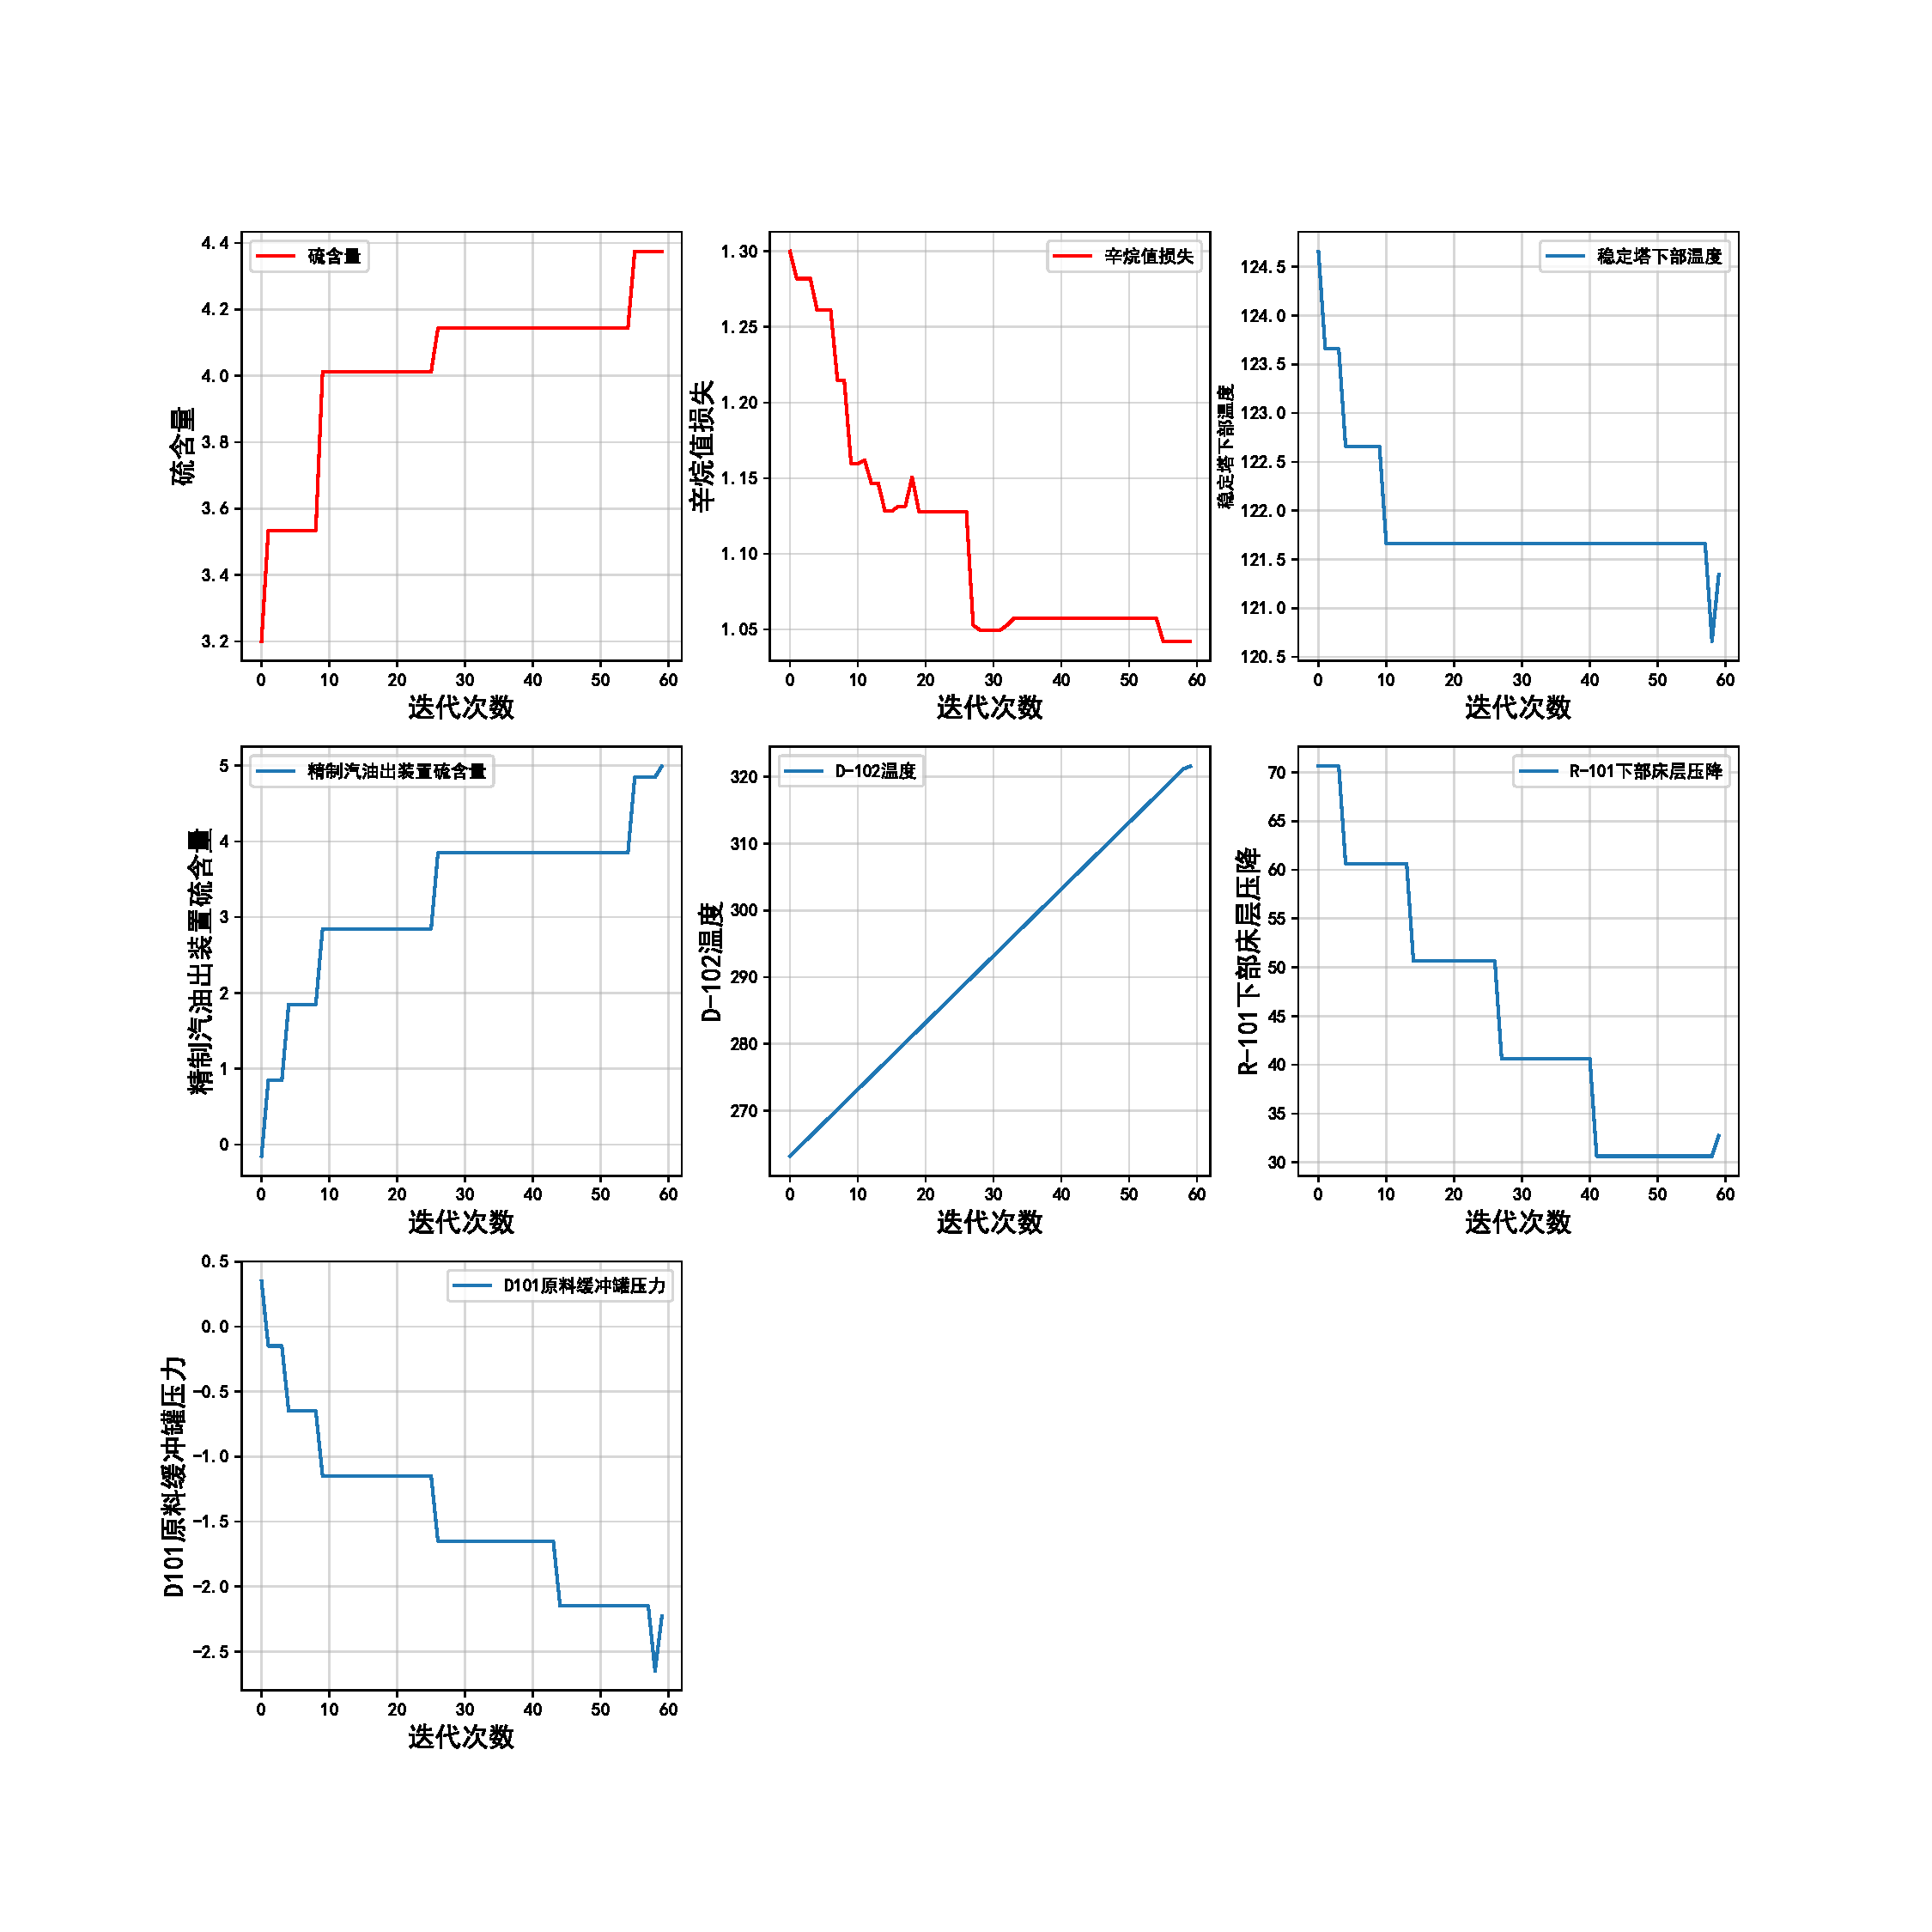
\includegraphics[width=1.0\textwidth]{first_it}
	\caption{第一轮迭代中硫产量、辛烷值损失及相应的五个操作变量随迭代次数变化的曲线}
\end{figure}


\begin{figure}[htb]
	\centering
	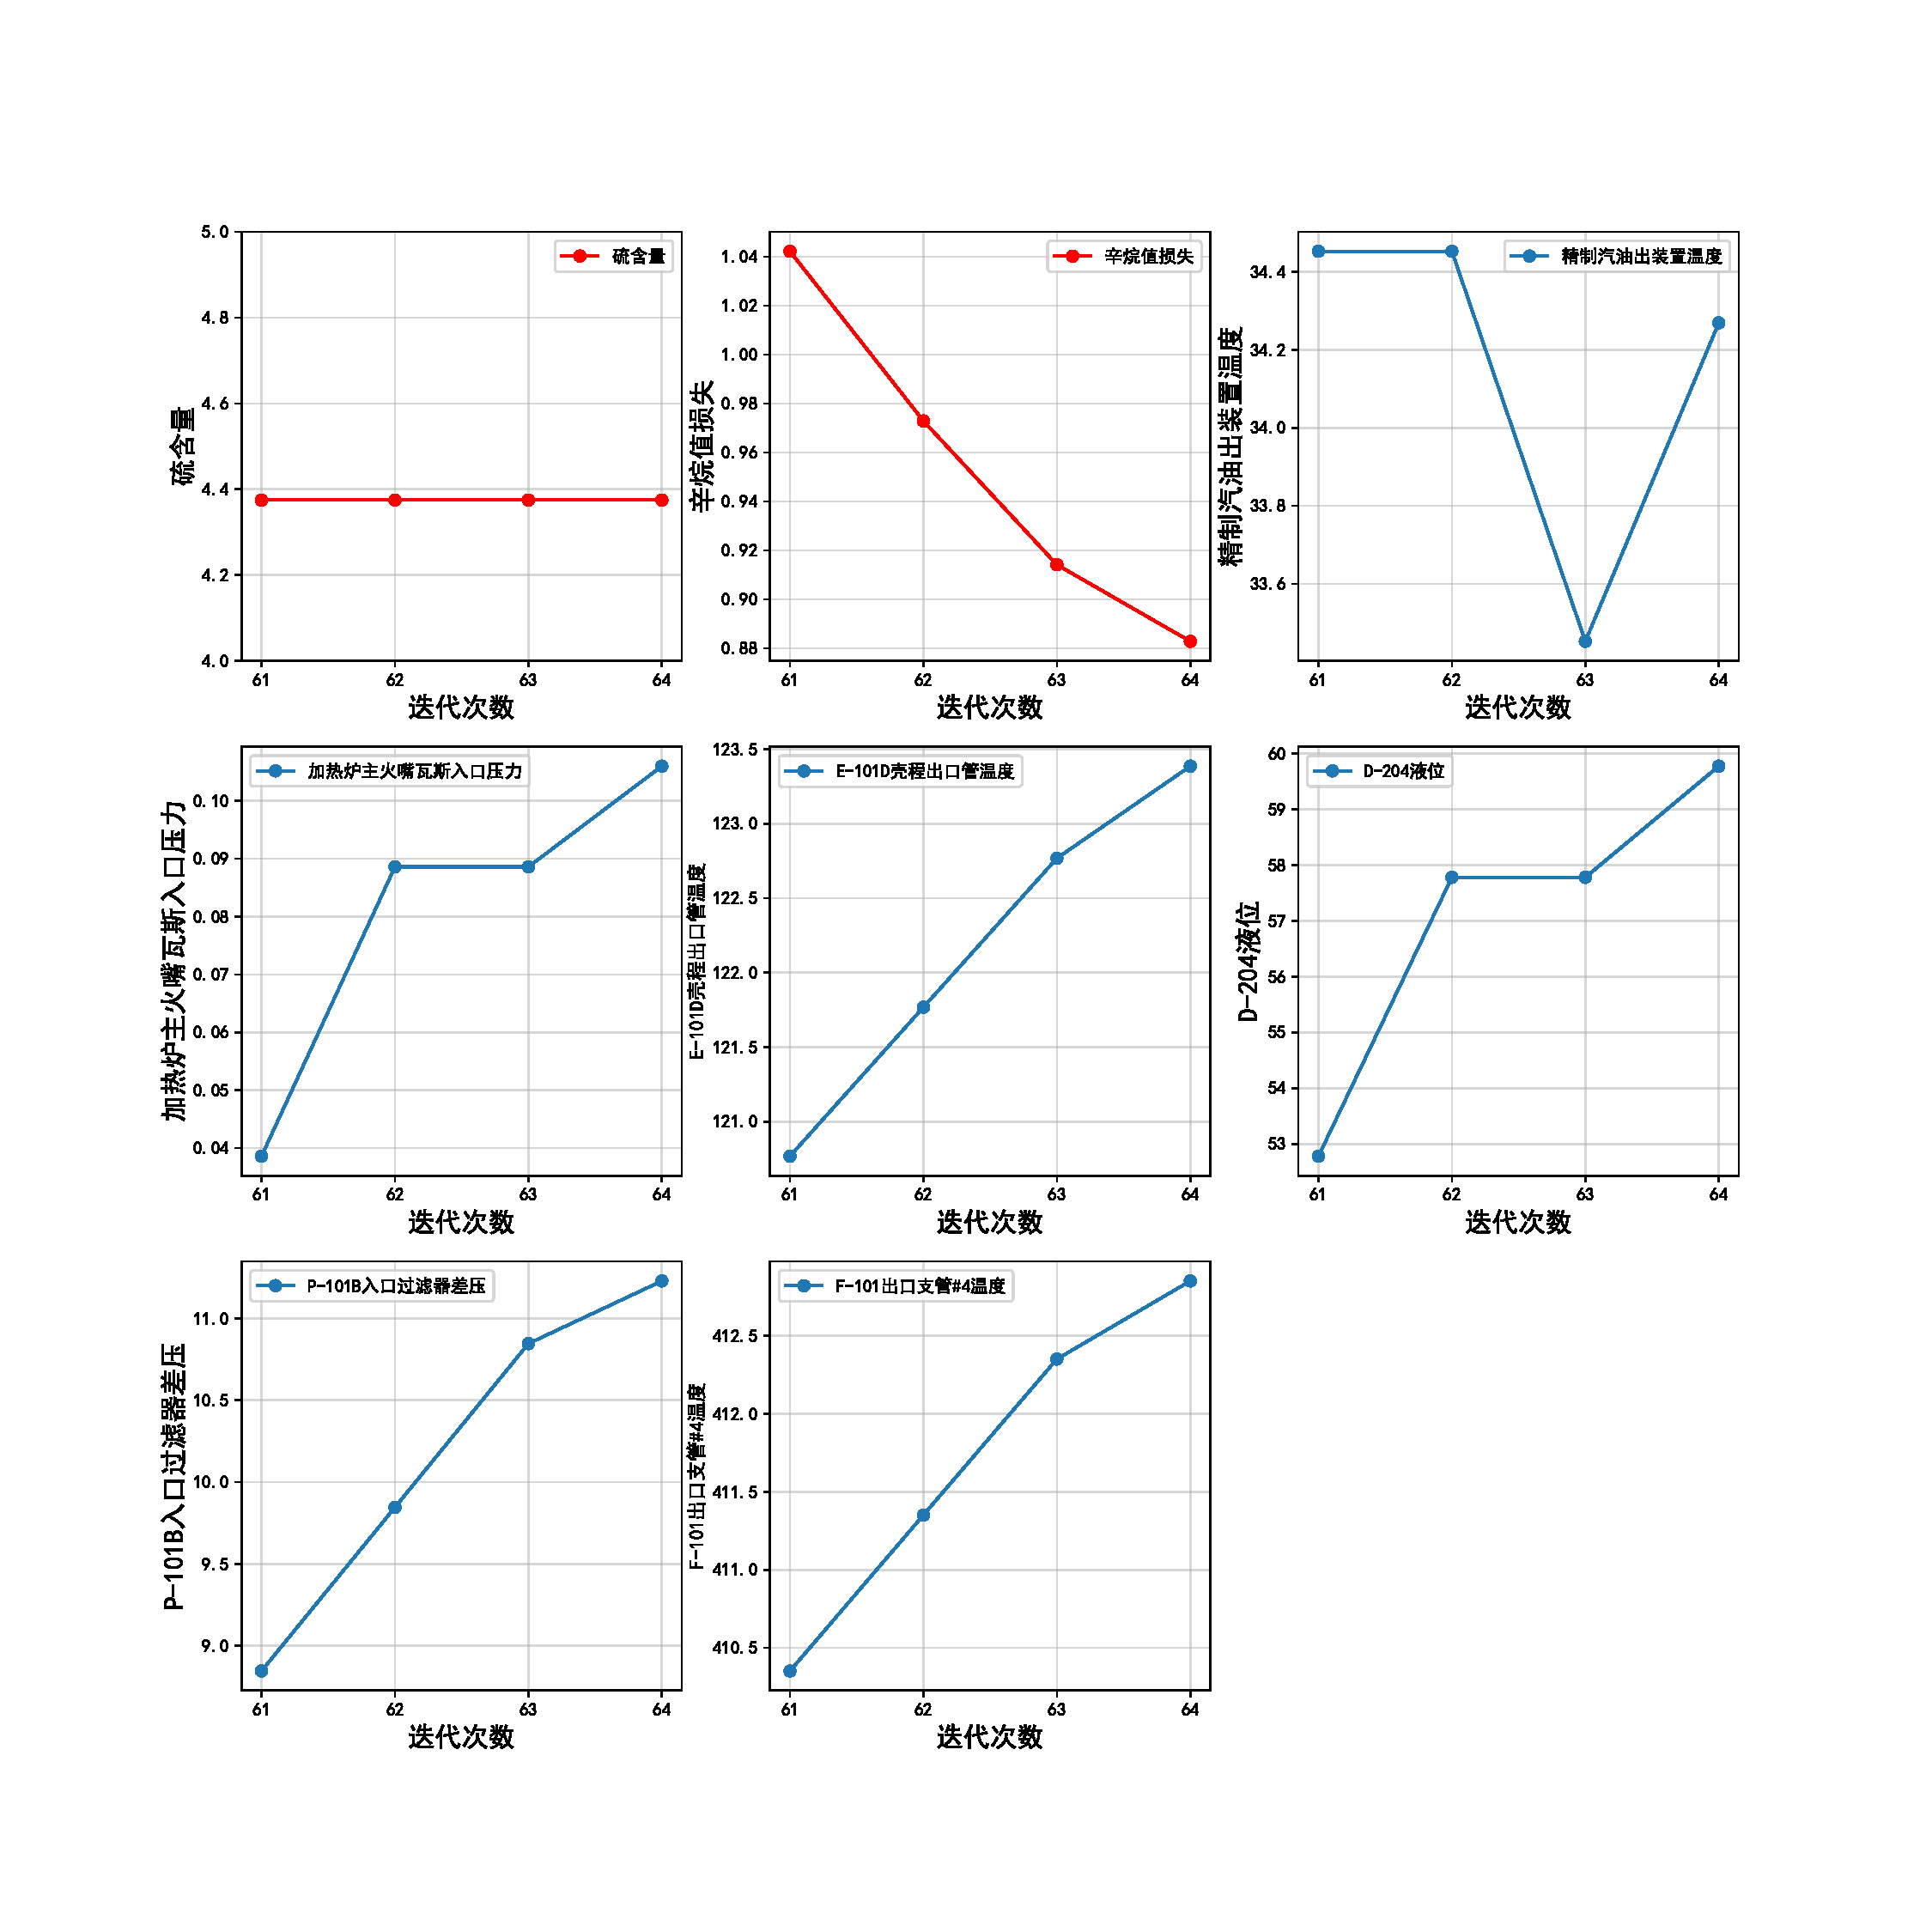
\includegraphics[width=1.0\textwidth]{second_it}
	\caption{第二轮迭代中硫产量、辛烷值损失及相应的五个操作变量随迭代次数变化的曲线}
\end{figure}


%第五章节
%下面这块看看怎么改
\FloatBarrier
\section{模型评价}


\FloatBarrier
\subsection{模型的优点}
\FloatBarrier
\subsubsection{问题一}
\begin{enumerate}[itemindent=20pt]
    \item 根据时序上是否平稳来决定313与285号样本的空值填充策略,灵活且具有自适应性。
    \item 通过公式定义操作变量的超出程度并以此为阈值删除采样样本,用3$\sigma$准则删除异常的采样样本,为下游操作提供鲁棒的模型。
    \item 根据不同场景制定对应的空值处理策略,灵活且高效。
\end{enumerate}

\FloatBarrier
\subsubsection{问题二}
\begin{enumerate}[itemindent=20pt]
    \item 用嵌入式的特征打分模型梯度提升树对特征进行评价,计算高效,结果可靠。
    \item 对比不同的特征筛选次数进一步限定主要变量的范围,科学且合理。
\end{enumerate}


\FloatBarrier
\subsubsection{问题三}
\begin{enumerate}[itemindent=20pt]
    \item 基于分布转换与LightGBM模型在12个主要变量的基础上建立RON损失模型,鲁棒且可泛化。
    \item 甄别出离群的异常样本并将其删除,提升了模型的综合表现。
\end{enumerate}


\FloatBarrier
\subsubsection{问题四}
\begin{enumerate}[itemindent=20pt]
    \item 根据产品硫含量不大于5$\mu$g/g的约束条件重新设计了评价函数,评价函数科学合理。
    \item 通过贝叶斯优化的TPE算法对325个样本的RON损失值进行优化,优化算法稳定高效。
\end{enumerate}

\FloatBarrier
\subsubsection{问题五}
\begin{enumerate}[itemindent=20pt]
    \item 对问题进行了合理的建模,求解出完全满足题目要求的修改路径,保证每次调整不超过$\Delta$允许的范围,每次调整不会超出操作变量的可行域,每次调整不会让硫产量大于5$\mu$g/g,最终实现辛烷值损失降低32.61\%。
    \item 对问题进行了合理简化,将连续变化的操作变量离散化处理,有利于使用启发式搜索算法,同时减少了计算量。
    \item 模型创新性的使用两步迭代算法,进一步简化模型,极大的减少了运算量缩短了运算时间,同时保证结果的正确性。
\end{enumerate}


\FloatBarrier
\subsection{模型的缺点}

\FloatBarrier
\subsubsection{问题一}
\begin{enumerate}[itemindent=20pt]
    \item 数据的空值等异常情况错综复杂,当前的处理策略可能难以覆盖所有的情况。
\end{enumerate}

\FloatBarrier
\subsubsection{问题二}
\begin{enumerate}[itemindent=20pt]
    \item 特征筛选的粒度还不够细,当前得到的12个主要变量可能不是最优的。
\end{enumerate}


\FloatBarrier
\subsubsection{问题三}
\begin{enumerate}[itemindent=20pt]
    \item 没有做超参优化与集成学习,模型的表现可能不是最优的。
\end{enumerate}


\FloatBarrier
\subsubsection{问题四}
\begin{enumerate}[itemindent=20pt]
    \item 贝叶斯优化可能不能在限定的优化次数中找到全局最优解。
\end{enumerate}

\FloatBarrier
\subsubsection{问题五}

\begin{enumerate}[itemindent=20pt]
    \item 为了减少搜索空间每次改变操作变量都是按照固定的值Δ调整,而实际操作中可以按照连续值调整自由度更高。
    \item 两步迭代的算法可能无法找到最短修改操作变量的路径。
\end{enumerate}





\newpage



% \section{加图的方法,记得删除}
% \begin{figure}[htb]
% \centering
% 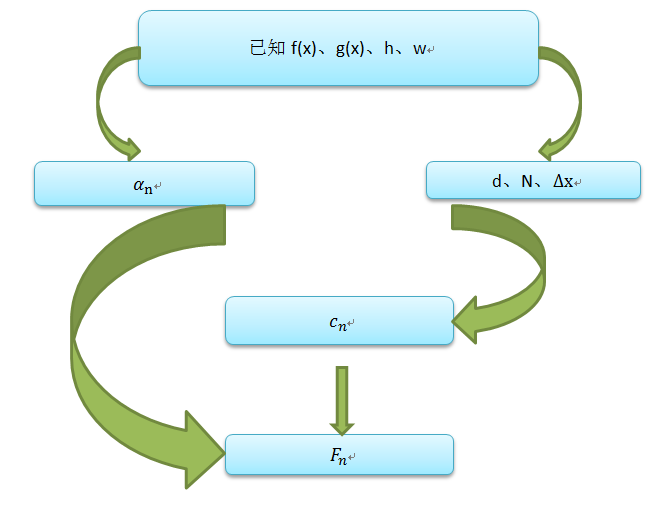
\includegraphics[width=.7\textwidth]{f1.png}
% \caption{问题三流程图}
% \end{figure}


%下面两种参考文献的格式二选一

%参考文献重新分页


% 参考文献   手工录入
% \begin{thebibliography}{9}%宽度9
% \bibitem{bib:one} ....
% \bibitem{bib:two} ....
% \end{thebibliography}

\newpage
\begin{thebibliography}{99}  
\bibitem{ref1}Pedregosa, F. and Varoquaux, G. and Gramfort, A. and Michel, V.
         and Thirion, B. and Grisel, O. and Blondel, M. and Prettenhofer, P.
         and Weiss, R. and Dubourg, V. and Vanderplas, J. and Passos, A. and
         Cournapeau, D. and Brucher, M. and Perrot, M. and Duchesnay, E., Scikit-learn: Machine Learning in {P}ython, America: Journal of Machine Learning Research, 2825--2830:2011。


% \bibitem{ref2}Arandjelović R, Zisserman A, Three things everyone should know to improve object retrieval, Computer Vision and Pattern Recognition (CVPR), 2012 IEEE Conference on, IEEE, 2012: 2911-2918.  
% \bibitem{ref3}Lowe D G. Distinctive image features from scale-invariant keypoints, International journal of computer vision, 2004, 60(2): 91-110.  
 \bibitem{ref4}Hua Zhu ,[算法]图解A\* 搜索算法, https:\/\/blog.csdn.net\/JasonZhu\_csdn\/article\/details\/86266228,2020年9月21日。

 \end{thebibliography}


% \bibitem{ref1}Zheng L, Wang S, Tian L, et al., Query-adaptive late fusion for image search and person re-identification, Proceedings of the IEEE Conference on Computer Vision and Pattern Recognition, 2015: 1741-1750.  

% %采用bibtex方案
% \cite{mittelbach_latex_2004,wright_latex3_2009,beeton_unicode_2008,vieth_experiences_2009}

% \bibliographystyle{gmcm}
% \bibliography{example}


% %参考文献 2019年大学生数学建模比赛的模板中提取的
% \begin{thebibliography}{9}%宽度9
%     \bibitem{1}{liuhaiyang2013latex}
%     刘海洋.
%     \newblock \LaTeX {}入门\allowbreak[J].
%     \newblock 电子工业出版社, 北京, 2013.
%     \bibitem{2}{mathematical-modeling}
%     全国大学生数学建模竞赛论文格式规范 (2020 年 8 月 25 日修改).
%     \bibitem{3} \url{https://www.latexstudio.net}
% \end{thebibliography}



% ?????????记得删掉
% @article{scikit-learn,
%  title={Scikit-learn: Machine Learning in {P}ython},
%  author={Pedregosa, F. and Varoquaux, G. and Gramfort, A. and Michel, V.
%          and Thirion, B. and Grisel, O. and Blondel, M. and Prettenhofer, P.
%          and Weiss, R. and Dubourg, V. and Vanderplas, J. and Passos, A. and
%          Cournapeau, D. and Brucher, M. and Perrot, M. and Duchesnay, E.},
%  journal={Journal of Machine Learning Research},
%  volume={12},
%  pages={2825--2830},
%  year={2011}
% }




\newpage
%附录
\appendix
%\setcounter{page}{1} %如果需要可以自行重置页码。
\section{我的 Python 源程序}
\begin{lstlisting}[language=Python]%设置不同语言即可。



 \end{lstlisting}



\end{document} 